\documentclass[12pt]{article}

% --------------
% setup packages
% --------------
\usepackage[english]{babel} % set default language to English
\usepackage[margin=.8in,top=1.1in,bottom=1.1in]{geometry} % page layout
\usepackage{amsmath,amsthm,amssymb,amsfonts} % math things
\usepackage{graphicx} % include graphics
\usepackage{titlesec} % help with section naming
\usepackage{xcolor} % color text [+ in math mode]
\usepackage{caption}
\usepackage{subcaption}
\usepackage{bookmark}
\usepackage{epsfig}
\usepackage[nottoc,numbib]{tocbibind} % add references to ToC
\usepackage{pifont} % for xmark == ding{53}
\usepackage{empheq} % for colorbox
\usepackage{mdframed} % for box around figures

\hypersetup{bookmarksopen=false,bookmarksnumbered=true}
\hypersetup{colorlinks=true,urlbordercolor=magenta}

% -------------
% custom colors
% -------------
\definecolor{darkgray}{RGB}{100, 100, 100}
\definecolor{darkergray}{RGB}{66, 66, 66}
\definecolor{gray}{rgb}{0.5,0.5,0.5}
\definecolor{orange}{rgb}{1.0,0.3,0.01}
\definecolor{violet}{rgb}{0.4,0.0,0.6}
\definecolor{yellow}{rgb}{1.0,0.7,0.0}
\definecolor{boxc}{rgb}{1.0, 1.0, .9}
\definecolor{mygreen}{rgb}{0, 0.75, 0.18}

% ----------------
% custom shortcuts
% ----------------
\renewcommand{\l}{\left}
\renewcommand{\r}{\right}
\renewcommand{\b}[1]{\textbf{\textit{#1}}}
\renewcommand{\t}[1]{\widehat{#1}}
\renewcommand{\u}[1]{\underline{#1}}
\newcommand{\bs}[1]{\boldsymbol{#1}}
\newcommand{\mb}[1]{\mathbf{#1}}
\newcommand{\mc}[1]{\mathcal{#1}}
\newcommand{\tb}[1]{\textbf{#1}}
\def\bg#1\eg{%
    \begin{gather}%
    #1%
    \end{gather}%
}

% --------------
% custom symbols
% --------------
\newcommand{\E}{\mathbb{E}}
\newcommand{\D}{\mathbb{D}}
\newcommand{\N}{\mathbb{N}}
\newcommand{\R}{\mathbb{R}}
\renewcommand{\P}{\mathbb{P}}

% ---------------
% custom commands
% ---------------
\newcommand{\boldmm}[1]{\textbf{\textit{#1}}}
\newcommand{\comment}[1]{ \color{darkgray}\left[\text{#1}\right]\color{black}}
\newcommand{\commenttwo}[2]{\color{darkgray}\left[\begin{array}{c}\text{#1}\\ \text{#2}\end{array}\right]\color{black}}
\newcommand{\gooditem}{\item[\checkmark]}
\newcommand{\baditem}{\item[\ding{53}]}
\newcommand{\evalat}[1]{\biggr\rvert _{#1}}
\newcommand{\bad}{\textbf{\color{red}[\ding{53}]} }
\newcommand{\good}{\textbf{\color{green}[\checkmark]} }

% ---------
% color box
% ---------
\newlength\mytemplen
\newsavebox\mytempbox

\makeatletter
\newcommand\mybox{%
    \@ifnextchar[%]
       {\@mybox}%
       {\@mybox[0pt]}}

\def\@mybox[#1]{%
    \@ifnextchar[%]
       {\@@mybox[#1]}%
       {\@@mybox[#1][0pt]}}

\def\@@mybox[#1][#2]#3{
    \sbox\mytempbox{#3}%
    \mytemplen\ht\mytempbox
    \advance\mytemplen #1\relax
    \ht\mytempbox\mytemplen
    \mytemplen\dp\mytempbox
    \advance\mytemplen #2\relax
    \dp\mytempbox\mytemplen
    \colorbox{boxc}{\hspace{0em}\usebox{\mytempbox}\hspace{0em}}}

\makeatother

% --------------
% begin document
% --------------
\begin{document}
	\pagenumbering{arabic}
	\begin{titlepage}
		\vspace*{0.1\paperheight}
		\centering
		\vspace*{8em}
		{\Huge \textbf{Boltzmann Machines}}\\
		\vspace*{1em}
		{\Large Yelysei Bondarenko}
		\vspace{0.2\paperheight}
	\end{titlepage}

	\pdfbookmark{Contents}{contents}
	\tableofcontents
	\setcounter{page}{1}
	
	\newpage
\section{Boltzmann Machines and RBMs}

\subsection{Before BMs\cite{rojas1996hopfield, hopfield, coursera_nn}}

\subsubsection{General RNNs}
In early 1980-x general \textbf{recurrent neural networks} (RNNs), described by (general) \emph{asyclic} graph began to arise.
\begin{itemize}
\item     mostly binary units, $\{0, 1\}$ (or $\{-1, 1\}$);
\gooditem signal feedback $\Rightarrow$ \textbf{memory} compared to FF NNs (more specifically, \emph{content-addressable memory} (CAM) $\Leftrightarrow$ weights themselves are used to store patterns);
\baditem  in general if activations are non-linear function they are hard to train (oscillations and chaotic behavior).
\end{itemize}

\begin{figure}[h]
\begin{mdframed}
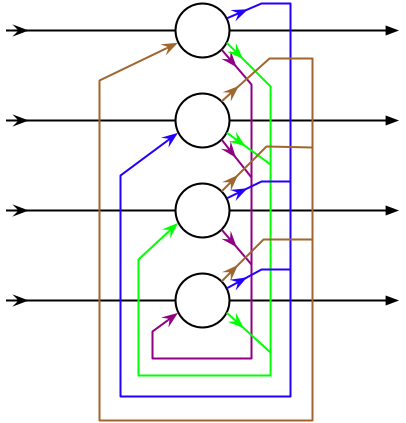
\includegraphics[scale=0.4]{img/general_rnn.png}
\centering
\caption{Example architecture of RNN}
\label{fig:general_rnn}
\end{mdframed}
\end{figure}

\vspace{1em}
\subsubsection{Hopfield Nets}
Later in $\approx$1982 John Hopfield has shown that if RNN has symmetric weights ($W_{ij}=W_{ji}$), and has no self-loops ($W_{ii}=0$), network's dynamics \textbf{is guaranteed} to converge to some stationary state. Fully-connected variant (complete graph) of such a network is called a \emph{Hopfield Network}.

Moreover, he also shown that each state of the Hopfield Net is associated with a scalar value referred to as the \emph{energy} of the network ($s_{i}\in\{-1, 1\}$ -- state of i-th neuron, $b_{i}$ -- bias of i-th neuron ($-b_{i}$ is activation threshold for the unit)):
\begin{align}
E = -\frac{1}{2}\sum_{i,j}W_{ij}s_is_j-\sum_{i}b_is_i=\commenttwo{$W_{ij}=W_{ji}$,}{$W_{ii}=0$} = -\sum_{i<j}W_{ij}s_is_j-\sum_{i}b_is_i
\end{align}
and local minima of $E(\mathbf{s};\mathbf{W}, \mathbf{b})\;\Leftrightarrow\;$ stable configurations of network. It is the first example of so-called \textbf{energy-based model}. Learning algorithm for such a model alter its (global) energy function to achieve desired properties. For instance, if a Hopfield Net is trained as autoassociator, the goal of learning is to shape energy function in such a way, that its local minima correspond to training examples (= patterns to "remember").
\begin{figure}[h]
\begin{mdframed}
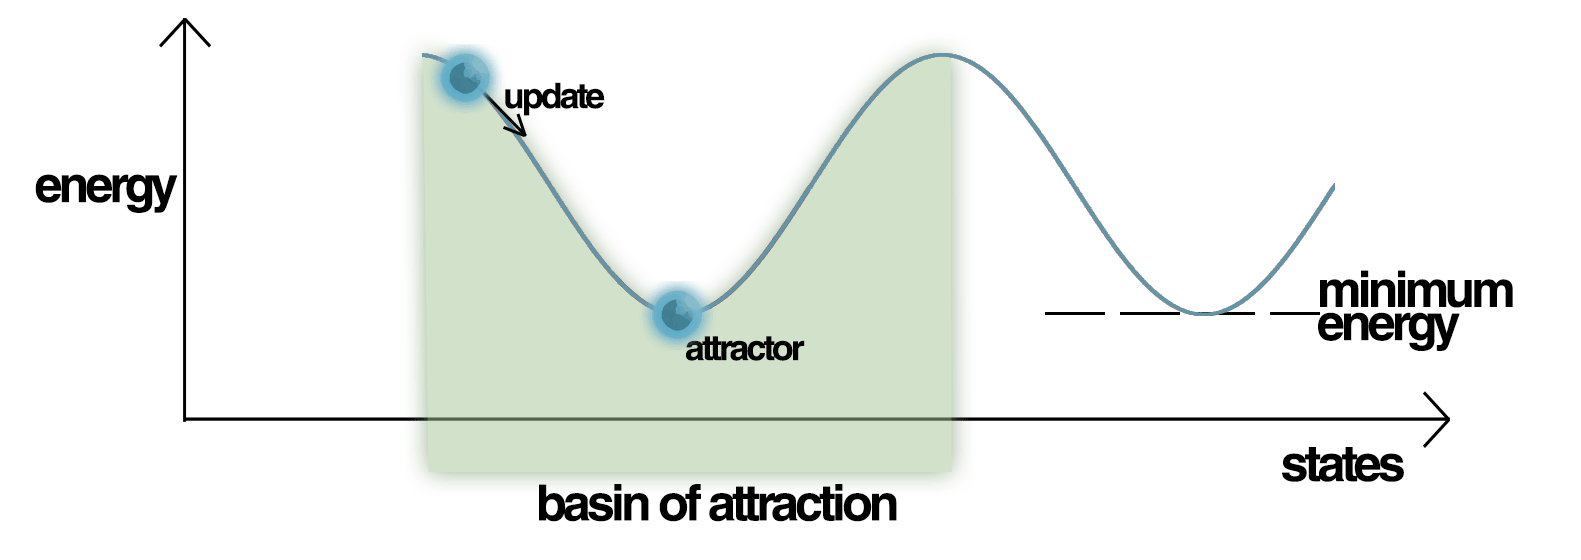
\includegraphics[scale=0.2]{img/energy_landscape.png}
\centering
\caption{Energy Landscape of a Hopfield Network, highlighting the current state of the network (up the hill), an attractor state to which it will eventually converge, a minimum energy level and a basin of attraction shaded in green. Note how the update of the Hopfield Network is always going down in Energy.}
\label{fig:energy_landscape}
\end{mdframed}
\end{figure}

\vspace{1em}
\subsubsection{Learning algorithms for Hopfield Nets}
There are exist couple of learning algorithms for Hopfield Nets.
First, thanks to simple quadratic shape of $E$, it is straightforward to calculate how i-th neuron influences the global energy:
\begin{gather*}
\Delta E_i = E(\mathbf{s}|s_i=\text{off}) - E(\mathbf{s}|s_i=\text{on}) = E(\mathbf{s}|s_i=0) - E(\mathbf{s}|s_i=1) =\\= -\sum_{k<j}W_{kj}s_ks_j\evalat{s_i=0} -\sum_{j}b_js_j\evalat{s_i=0}  + \sum_{k<j}W_{kj}s_ks_j\evalat{s_i=1} + \sum_{j}b_js_j\evalat{s_i=1} =\\=
\underbrace{-\l( \sum_{k<j, k \neq i, j \neq i}W_{kj}s_ks_j + \sum_{j \neq i}b_js_j \r) + \l( \sum_{k<j, k \neq i, j \neq i}W_{kj}s_ks_j + \sum_{j \neq i}b_js_j \r)}_{=0} +
\underbrace{\sum_{j<i}W_{ji}s_j}_{k=i} + \underbrace{\sum_{i<k}W_{ik}s_k}_{j=i} + b_i =\\= \comment{$W_{ij}=W_{ji}$, $W_{jj}=0$} = \sum_jW_{ij}s_is_j + b_i
\end{gather*}
This lead to the learning algorithm called \textbf{Binary Threshold Decision Rule} (BTDR):
\begin{itemize}
\item Randomly initialize states (or to desired pattern if want CAM);
\item While not converged or for fixed number of iterations:
	\subitem For each neuron:
		\subsubitem Change its state if this will decrease global energy. More specifically:
		 $$
		 s_i \leftarrow
		 \begin{cases}
		 +1,  \;\;\Delta E_i > 0,\\
		 s_i, \;\;\Delta E_i = 0,\\
		 -1,  \;\;\Delta E_i < 0.\\
		 \end{cases}
		 $$
\end{itemize}
This learning algorithm is \emph{local} and \emph{incremental}, thus biologically plausible. Also neurons could have been updated simultaneously, but it is less likely that there is exists "global clock" in biological system, and such kind of updates can also cause oscillation or chaotic behavior.

One important \underline{drawback} of such an algorithm, is that once we stuck in poor local minimum, we cannot escape it, it is also one of the reasons why Boltzmann Machines was more successful.

\vspace{2em}
Another learning algorithm is based on famous \textbf{Hebb rule}: "Cells that fire together, wire together". In the simplest case it simply says:
\begin{gather}
W_{ij} \leftarrow x_ix_j,
\end{gather}
where $\mathbf{x}=\{x_1 \ldots x_N\}$ is binary input pattern. If $x_i$ and $x_j$ are the same, then $W_{ij}$ is positive thus i-th and j-th state tend to become equal. Opposite happens when $x_i$ and $x_j$ are different. Now one can show that network's dynamics will be the same if
\begin{gather}
W_{ij} \leftarrow \frac{1}{N}x_ix_j
\end{gather}
If we need to remember not 1 but $P$ patterns, sum corresponding update for each pattern (for each pattern pretend there are no others):		
\begin{gather}
W_{ij} \leftarrow \frac{1}{N}\sum_{p=1}^Px_i^{(p)}x_j^{(p)}
\end{gather}
This way network will act as CAM, see Fig. \ref{fig:hopfield}. The network will converge to a "remembered" state if it is given only part of the state $\Rightarrow$ can be used to recover from a distorted input to the trained state that is most similar to the input.
\begin{figure}[h]
\begin{mdframed}
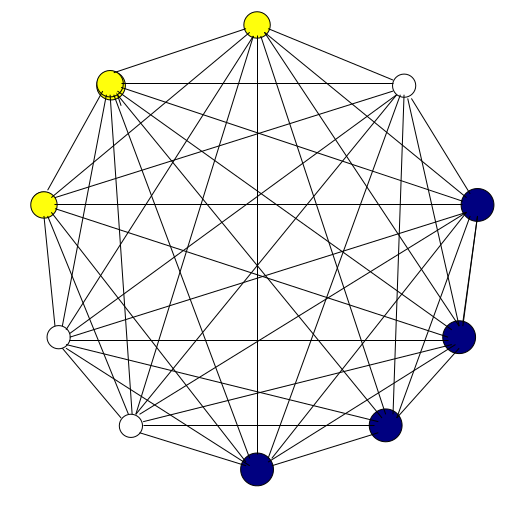
\includegraphics[scale=0.4]{img/hopfield.png}
\centering
\caption{A Hopfield network as an autoassociator. One enters a pattern in
blue nodes and let the network evolve. After a while one reads out the yellow
nodes. The memory of the Hopfield network associates the yellow node pattern
with the blue node pattern.}
\label{fig:hopfield}
\end{mdframed}
\end{figure}

\vspace{1em}
For instance, train Hopfield net such that $(1, -1, 1, -1, 1)$ is a local minimum of $E$ (phase 1 -- memorization). Next, if the network is properly trained, it can recover $(1, -1, 1, -1, 1)$ from $(1, -1, \mathbf{-1}, -1, 1)$ input (phase 2 -- recognition). Hopfield nets can be used for denoising of simple fonts.	

\vspace{1em}
Many generalizations of this rule exist, but fundamentally Hopfield nets had quite some drawbacks (even for binary data):
\begin{itemize}
\baditem patterns are stored in the network itself, thus can be intractable for large $N$;
\baditem capacity, one can reliably store only $P << N$ patterns;
\baditem spurious minima, poor local minima;
\baditem no probabilistic interpretation.
\end{itemize}
But anyway Hopfield Nets and energy-based models played a big role in development of deep learning and now we proceed to the one of the most famous modification of Hopfield Net -- Boltzmann Machine.

\subsection{Boltzmann Machines\cite{coursera_nn, aarts1988simulated, fischer2012introduction, tutorial2014lisa}}
\subsubsection{Main ideas}
Boltzmann Machine (developed $\approx$1980-85 by G. Hinton) is a \emph{stochastic}, \emph{generative} counter-part of Hopfield Nets. From PGM point of view, it is an example of MRF (undirected graphical model). It is also an example of Ising model.
\\[1em]
Two main ideas:
\begin{enumerate}
\item Instead of storing "memories" in stable configurations of Hopfield net, use them for "interpretation" of the input data. Thus, all units are divided into 2 groups: \emph{visible} and \emph{hidden} (see Fig. \ref{fig:bm}).
\begin{figure}[h]
\begin{mdframed}
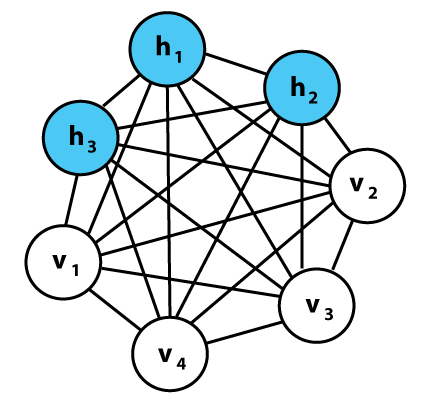
\includegraphics[scale=0.4]{img/bm.png}
\centering
\caption{A graphical representation of an example Boltzmann machine. Each undirected edge represents dependency. In this example there are 3 hidden units and 4 visible units. This is not a restricted Boltzmann machine.}
\label{fig:bm}
\end{mdframed}
\end{figure}

\item To escape local minima, assume units are \emph{Gibbs distibuted} with the same energy function (1) and use more advanced learning algorithms (see below).
\end{enumerate}

\subsubsection{Historical development and informal explanation}
Inspired from statistical physics, assume that units' states are Gibbs distributed (= Boltzmann distributed) random variables for global energy (1) $\;\Rightarrow\;$ energy of the state is proportional to the negative log-probability of that state and also the following identity holds:
\begin{gather}
\Delta E_i = E(\mathbf{s}|s_i=0) - E(\mathbf{s}|s_i=1) \;\propto\; -k_BT\log p\{s_i=0\}+k_BT\log p\{s_i=1\},
\end{gather}
By absorbing Boltzmann's constant $k_B$ into introduced notion of (artificial) temperature $T$ ($T\leftarrow k_BT$) ($\Leftrightarrow$ by considering \emph{dimensionless} units where $k_B=1$) , we can rearrange equation (5) and solve for $ p\{s_i=1\}$. We will obtain so-called \emph{normal logistic equation}:
\begin{gather}
 p\{s_i=1\}=\frac{1}{1+\exp\l(-\frac{\Delta E_i}{T}\r)}=\text{sigm}\l(-\frac{\Delta E_i}{T}\r)
\end{gather} 
We obtained a \textbf{Modified BTDR}:
\begin{itemize}
\item Randomly initialize states;
\item In cycle for each unit if its state reversal will yield energy decrease, reverse its state with probability described by (6).
\end{itemize}
After running for long enough time at certain $T$, it turns out that probability of a global state of network will \emph{depend only upon global state's energy}, and not on the initial state (in accordance with Boltzmann distribution). 
\\$\Rightarrow$ Distribution of all possible configurations (global states) converges to same \emph{stationary distribution} (this state in physics is called thermal equilibrium). Note that being in thermal equilibrium, system does not necessary is in the state of the lowest energy, which still might be oscillating, \textbf{but} if we start running the network from a high temperature, and gradually decrease it over time until we reach a thermal equilibrium at low $T$, we may converge to a distribution where the energy level fluctuates around the global minimum (at least this can happen with higher probability than in Hopfield Nets). 
\\This process is called \textbf{simulated annealing}. Yes, it seems like development of BMs gave fundament to one of the most famous and successful algorithms of global optimization.
\\[1em]
Now if we want to train the network so that the chance it will converge to a global state is according to an external distribution (e.g. data) that we have over these states, we need to \emph{set the weights} so that the global states with the highest probabilities will get the lowest energies. By altering parameters we can shape the distribution produced by BM using (6), it is the main idea of Boltzmann machine.
\\[1em]
BM is interpreted in the following way. Visible units provide open interface to the world and represent data. Hidden units represent hidden patterns in the data. Usually it is trained by using maximum likelihood estimation using approximate (why see below) gradient ascent. It is also equivalent \cite{goodfellow2016deep} to minimizing KL-divergence between external distribution (which is usually empirical data distribution) and model distribution produced by the network.

\subsubsection{More formal derivations}
\u{Notations}:
\\$\mathbf{v}\in\{0,1\}^D=\{0,1\}^V$ -- vector of visible units,
\\$\mathbf{h}\in\{0,1\}^H$ -- vector of hidden units,

Energy of a particular state $(\mathbf{v},\mathbf{h})$ is:
\begin{gather}
E(\mathbf{v},\mathbf{h};\bs{\psi})=-\frac{1}{2}\mb{v}^T\mb{L}\mb{v}-\frac{1}{2}\mb{h}^T\mb{J}\mb{h}-\mb{v}^T\mb{W}\mb{h}-\mb{b}^T\mb{v}-\mb{c}^T\mb{h},
\end{gather}
it is nothing else but (1) with old $\mb{W}$ split into $\mb{L}$ describing vis-vis weights, $\mb{J}$ describing hid-hid weights, and new $\mb{W}$ describing vis-hid connections, and the same for biases. The reason is to keep notations consistent with later parts where we will get rid of $\mb{L}$ and $\mb{J}$. Of course, $\mb{L}$ and $\mb{J}$ are symmetric with zeros on the main diagonal. $\bs{\psi}=\{\mb{L},\mb{J},\mb{W},\mb{b},\mb{c}\}$ are model parameters.

Probability of the configuration $(\mb{v},\mb{h})$ is (according to the Boltzmann distribution):
\begin{gather}
p(\mathbf{v},\mathbf{h};\bs{\psi})=\frac{e^{-E(\mathbf{v},\mathbf{h};\bs{\psi})}}{\sum_{\mb{\t{v}},\mb{\t{h}}} e^{-E(\mathbf{\t{v}},\mathbf{\t{h}};\bs{\psi})} }=:\frac{p^*(\mb{v},\mb{h}; \bs{\psi})}{Z(\bs{\psi})},
\end{gather}
where $p^*(\mb{v},\mb{h}; \bs{\psi})$ is unnormalized probability of the configuration and $Z(\bs{\psi})$ is a normalizer also called \emph{partition function}.
\\$\Rightarrow$
\\Probability that model assigns to a visible vector $\mb{v}$ is
\begin{gather}
p(\mb{v};\bs{\psi})=\sum_{\mb{h}}p(\mathbf{v},\mathbf{h};\bs{\psi})=:\frac{e^{-\mathcal{F}(\mb{v};\bs{\psi})}}{\sum_{\mb{\t{v}}} e^{-\mathcal{F}(\mb{\t{v}};\bs{\psi})} },
\end{gather}
where
\begin{gather}
\mc{F}(\mb{v};\bs{\psi})=-\log\l( \sum_{\mb{h}}e^{-E(\mb{v},\mb{h};\bs{\psi})} \r)
\end{gather}
is called \emph{free energy} (\emph{free} because all the hidden states are marginalized out; the name is inspired again from physics), useful quantity which will be used later.
\\[1em]
\u{Now lets calculate} $p(v_i=1|\mb{h},\mb{v}_{-i})$: (omit $\bs{\psi}$ for brevity)

\begin{empheq}[box={\mybox[1em][1em]}]{gather*}
p(v_i=1|\mb{h},\mb{v}_{-i})=\frac{p(v_i=1,\mb{v}_{-i},\mb{h})}{p(\mb{v}_{-i},\mb{h})}=
\frac{p(v_i=1,\mb{v}_{-i},\mb{h})}{p(v_i=0,\mb{v}_{-i},\mb{h})+p(v_i=1,\mb{v}_{-i},\mb{h})}
\\=\frac{e^{-E(v_i=1,\mb{v}_{-i},\mb{h})}}{e^{-E(v_i=0,\mb{v}_{-i},\mb{h})} + e^{-E(v_i=1,\mb{v}_{-i},\mb{h})}}=\frac{1}{1+e^{-\l[E(v_i=0,\ldots)-E(v_i=1,\ldots)\r]}}=\text{sigm}\l[E(v_i=0,\ldots)-E(v_i=1,\ldots)\r]=
\\=\comment{$E(\mb{v},\mb{h})=-\sum_{j<k}L_{jk}v_jv_k -\sum_{l<m}J_{lm}h_lh_m -\sum_{j,l}W_{jl}v_jh_l-\sum_jb_jv_j-\sum_lc_lh_l $}=
\\=\comment{sums w/o $v_i$ (2nd, 5th) cancel out}=\text{sigm}\l[\underbrace{-\ldots+\sum_{j<k,j\neq i, k\neq i}L_{jk}v_jv_k}_{=0}+\underbrace{\sum_{i<k}L_{ik}v_k}_{j=i}+ \underbrace{\sum_{j<i}L_{ji}v_j}_{k=i} -\r.\\\l.\underbrace{-\ldots+\sum_{j\neq i, l}W_{jl}v_jh_l}_{=0}+  \underbrace{\sum_lW_{il}h_l}_{j=i}+b_i\r]=\comment{$L_{ij}=L_{ji}, L_{ii}=0$}=\text{sigm}\l[ \sum_lW_{il}h_l+\sum_kL_{ik}v_k+b_i \r]
\end{empheq}	
So:
\begin{gather}
\boxed{p(v_i=1|\mb{h},\mb{v}_{-i})=\text{sigm}\l( \sum_kL_{ik}v_k+\sum_lW_{il}h_l+b_i \r)}
\end{gather}
\u{Symmetrically},
\begin{gather}
\boxed{p(h_j=1|\mb{v},\mb{h}_{-j})=\text{sigm}\l( \sum_lJ_{jl}h_l+\sum_iW_{ij}v_i+c_j \r)}
\end{gather}
\\[1em]
\u{Maximum Likelihood learning}
\\Suppose we have dataset $\mc{D}=\{\mb{x}_1,\ldots\mb{x}_N\}, \mb{x}_n\in\{0,1\}^D$. The goal is to maximize $\sum_{n=1}^N\log p(\mb{x}_n;\bs{\psi})$ for parameters $\bs{\psi}$. For a single training example $\mb{v}$ and any parameter $\theta$:
\begin{empheq}[box={\mybox[1em][1em]}]{gather*}
\frac{\partial}{\partial\theta}\log p(\mb{v};\bs{\psi})=
\frac{\partial}{\partial\theta}\l(\log \sum_{\mb{h}}e^{-E(\mb{v},\mb{h};\bs{\psi})}-
\log\sum_{\mb{\t{v}},\mb{\t{h}}}e^{-E(\mb{\t{v}},\mb{\t{h}};\bs{\psi})} \r)=
\\=-\frac{1}{\sum_{\mb{h}}e^{-E(\mb{v},\mb{h};\bs{\psi})}}\sum_{\mb{h}}\l[e^{-E(\mb{v},\mb{h};\bs{\psi})} \cdot \frac{\partial}{\partial\theta}E(\mb{v},\mb{h};\bs{\psi}) \r]+
\frac{1}{\sum_{\mb{\t{v}},\mb{\t{h}}}e^{-E(\mb{\t{v}},\mb{\t{h}};\bs{\psi})}}
\sum_{\mb{\t{v}},\mb{\t{h}}}\l[e^{-E(\mb{\t{v}},\mb{\t{h}};\bs{\psi})}\cdot \frac{\partial}{\partial\theta} E(\mb{\t{v}},\mb{\t{h}};\bs{\psi}) \r]=
\\=\comment{$\frac{e^{-E(\mb{v},\mb{h};\bs{\psi})}}{\sum_{\mb{h}}e^{-E(\mb{v},\mb{h};\bs{\psi})}}=\frac{\frac{1}{Z(\theta)}e^{-E(\mb{v},\mb{h};\bs{\psi})}}{\frac{1}{Z(\theta)}\sum_{\mb{h}}e^{-E(\mb{v},\mb{h};\bs{\psi})}}=\frac{p(\mb{h},\mb{v};\bs{\psi})}{p(\mb{v};\bs{\psi})}=p(\mb{h}|\mb{v};\bs{\psi})$}=
\\=-\underbrace{\sum_{\mb{h}}p(\mb{h}|\mb{v};\bs{\psi})\cdot\frac{\partial}{\partial\theta}E(\mb{v},\mb{h};\bs{\psi})}_{\E_{\mb{h}|\mb{v};\bs{\psi}}\l[\frac{\partial}{\partial\theta}E(\mb{v},\mb{h};\bs{\psi})\r]}
+\underbrace{\sum_{\mb{\t{v}},\mb{\t{h}}}p(\mb{\t{v}},\mb{\t{h}};\bs{\psi})\cdot\frac{\partial}{\partial\theta}E(\mb{\t{v}},\mb{\t{h}};\bs{\psi})}_{\E_{\mb{\t{v}},\mb{\t{h}};\bs{\psi}}\l[\frac{\partial}{\partial\theta}E(\mb{\t{v}},\mb{\t{h}};\bs{\psi})\r]}
\end{empheq}
This we obtain
\begin{gather}
\boxed{\frac{\partial}{\partial\theta}\log p(\mb{v};\bs{\psi})=-\E_{\mb{h}|\mb{v};\bs{\psi}}\l[\frac{\partial E}{\partial\theta}(\mb{v},\mb{h};\bs{\psi})\r]+\E_{\mb{\t{v}},\mb{\t{h}};\bs{\psi}}\l[\frac{\partial E}{\partial\theta}(\mb{\t{v}},\mb{\t{h}};\bs{\psi})\r]}
\end{gather}
And avegared over all data points:
\begin{gather}
\frac{1}{N}\sum_{n=1}^N \frac{\partial}{\partial\theta} \log p(\mb{x}_n;\bs{\psi})=-\frac{1}{N}\sum_{n=1}^N \E_{\mb{h}|\mb{v};\bs{\psi}}\l[\frac{\partial E}{\partial\theta}(\mb{x}_n,\mb{h};\bs{\psi})\r] + \E_{\mb{\t{v}},\mb{\t{h}};\bs{\psi}}\l[\frac{\partial E}{\partial\theta}(\mb{\t{v}},\mb{\t{h}};\bs{\psi})\r]
\end{gather}
or solely in terms of expectations:
\begin{gather}
\boxed{\E_{\mb{v}\sim P_{\text{data}}(\mb{v})}\l[ \frac{\partial}{\partial\theta}\log p(\mb{v};\bs{\psi}) \r]=-\E_{\mb{v},\mb{h}\sim P_{\text{data}}(\mb{v},\mb{h};\bs{\psi})}\l[ \frac{\partial E}{\partial\theta}(\mb{v},\mb{h};\bs{\psi}) \r] + \E_{\mb{v},\mb{h}\sim P_{\text{model}}(\mb{v},\mb{h};\bs{\psi})}\l[ \frac{\partial E}{\partial\theta}(\mb{v},\mb{h};\bs{\psi}) \r]}
\end{gather}
where $P_{\text{data}}(\mb{v})=\frac{1}{N}\sum_{n=1}^N \delta_{\mb{v},\mb{x}_n}$ is \emph{empirical distribution}, $P_{\text{data}}(\mb{v},\mb{h};\bs{\psi})=p(\mb{h}|\mb{v};\bs{\psi})P_{\text{data}}(\mb{v})$ is \emph{complete-data distribution} and $P_{\text{model}}$ is a distribution modelled by BM.
\\[1em]
Before we move on, there is one more equivalent form of gradient of data log-likelihood:
\begin{gather}
-\frac{\partial}{\partial\theta}\log p(\mb{v};\bs{\psi})=\frac{\partial}{\partial\theta}\mc{F}(\mb{v})-\sum_{\mb{\t{v}}}p(\mb{\t{v}})\frac{\partial}{\partial\theta}\mc{F}(\mb{\t{v}})
\end{gather}
Notice that the above gradient contains two terms, which are referred to as the \textbf{positive} and \textbf{negative} phase. The terms positive and negative do not refer to the sign of each term in the equation, but rather reflect their effect on the probability density defined by the model. The first term increases the probability of training data (by reducing the corresponding free energy), while the second term decreases the probability of samples generated by the model.
\\[1em]
\u{Derivatives of the energy w.r.t. model parameters}:
$$
E(\mathbf{v},\mathbf{h};\bs{\psi})=-\frac{1}{2}\mb{v}^T\mb{L}\mb{v}-\frac{1}{2}\mb{h}^T\mb{J}\mb{h}-\mb{v}^T\mb{W}\mb{h}-\mb{b}^T\mb{v}-\mb{c}^T\mb{h},
$$
\begin{itemize}
\item $\frac{\partial E}{\partial \mb{L}}=-\mb{v}\mb{v}^T$ (remember that $\mb{L}$ is symmetric)
\item Similarly $\frac{\partial E}{\partial \mb{J}}=-\mb{h}\mb{h}^T$ and $\frac{\partial E}{\partial \mb{W}}=-\mb{v}\mb{h}^T$
\item Finally $\frac{\partial E}{\partial \mb{b}}=-\mb{v}$ and $\frac{\partial E}{\partial \mb{c}}=-\mb{h}$
\end{itemize}
So 1 update of the weights $\mb{W}$ using vanilla gradient ascent looks like:
\begin{align}
\mb{g}_{\mb{W}} &\;\leftarrow\; \E_{\mb{v},\mb{h}\sim P_{\text{data}}(\mb{v},\mb{h};\bs{\psi})}\l[\mb{v}\mb{h}^T\r]-\E_{\mb{v},\mb{h}\sim P_{\text{model}}(\mb{v},\mb{h};\bs{\psi})}\l[\mb{v}\mb{h}^T\r]
\\ 
\mb{W} &\;\leftarrow\; \mb{W} + \alpha\cdot\mb{g}_{\mb{W}}
\end{align}
and similarly for other parameters.
\\[1em]
\u{Problems}
\\
So far it seems like everything is ok, but there is 1 very serious problem, \textbf{both expectations in (13) $\Leftrightarrow$ (15) are simply intractable}. First sum has $O\l(2^H\r)$ terms while the second one has $O\l(2^{V+H}\r)$ terms. Moreover, even $p(\mb{h}|\mb{v};\bs{\psi})$ or $p(\mb{v},\mb{h};\bs{\psi})$ are intractable because of partition function in denominators which itself has exponentially many in $V+H$ terms.
\\[1em]To overcome this computational burden, G. Hinton and T. Sejnowski in 1983 proposed algorithm that uses Gibbs sampling to approximate both expectations. The idea is that both expectations are approximated by states of 2 Markov chains (Monte-Carlo sampling), which are updated using Gibbs sampling $\forall$ training example during training.
\\[1em]The main problem with the last algorithm is \tb{time} required to approach distribution, especially when estimating the model's expectations, since the Gibbs chain may need to explore a highly multimodal energy landscape + exponential in machine size and magnitude of weights time to collect equilibrium statistics. We will see that in RBM Gibbs sampling can be performed much more efficiently thus having much more efficient learning algorithm.
\\[1em]
To summarize, Boltzmann Machines is a Monte Carlo version of Hopfield Net with discrimination between visible and hidden units and that uses annealed Gibbs sampling. Boltzmann Machines were one of the first neural networks capable of learning internal representations, and are able to represent and (given sufficient time) solve difficult combinatoric problems + they are again are considered a biologically plausiable because during learning only local information is used, i.e. the update for a particular weight connecting two units depend only on the statistics of those two units (this can be seen by considering equation (17) element-wisely).
\subsubsection{Additional facts}
\textbullet{} from formulae (11),(12) we can see that probability of one unit being on is given by a linear model (logistic regression) from the values of the other units.
\\
\textbullet{} in the presence of hidden units, BM becomes a \emph{universal approximator} in a sense that it can learn arbitraty point mass function over discrete variables (without hidden units it could have learned only linear relationships between variables) \cite{goodfellow2016deep}
\\
\textbullet{} it is also interesting that in this model we can compute $p(\mb{h}|\mb{v};\bs{\psi})$ exactly and efficiently, unlike many other models with hidden variables like VAE etc., and still this model can learn fairly complex distributions (+ previous bullet)

\subsection{Restricted Boltzmann Machines\cite{coursera_nn, fischer2012introduction, tutorial2014lisa, hinton2010practical, fischer2014training, smolensky1986information, gibbs_wiki}}
\subsubsection{Intro and comparison with general BM}
A \emph{restricted Boltzmann machine} was invented by P. Smolensky in 1986 and is characterized by absense of hid-hid and vis-vis connections (see Fig. \ref{fig:rbm}).
\begin{figure}[h]
\begin{mdframed}
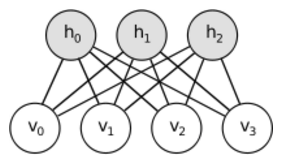
\includegraphics[scale=0.5]{img/rbm.png}
\centering
\caption{Diagram of a restricted Boltzmann machine with four visible units and three hidden units (no bias units).}
\label{fig:rbm}
\end{mdframed}
\end{figure}
In this case we have $\mb{L}=\mb{J}=\mb{0}$ and the energy function for RBM simplifies:
\bg
E(\mathbf{v},\mathbf{h};\bs{\psi})=-\mb{v}^T\mb{W}\mb{h}-\mb{b}^T\mb{v}-\mb{c}^T\mb{h}
\eg
Because of the \emph{bipartite} structure of the graph, in this MRF \tb{all hidden units are conditionally independent given visible ones and vice versa} ($\bs{\psi}$ is omitted for brevity):
\bg
p(\mb{h}|\mb{v})=\prod_jp(h_j|\mb{v}), \;\;\; p(\mb{v}|\mb{h})=\prod_ip(v_i|\mb{h})
\eg
(Formally every path in this graphical model between different $h_j$ and $h_l$ is blocked by $\mb{v}$ and vice versa).
\\[1em]
Taking this into account, formulae (11) and (12) simplify too:
\bg
p(v_i=1|\mb{h})=\text{sigm}\l( \sum_lW_{il}h_l+b_i \r),
\\
p(h_j=1|\mb{v})=\text{sigm}\l( \sum_iW_{ij}v_i+c_j \r)	
\eg
very important that each of these formulae can be computed \tb{in parallel}:
\bg
p(\mb{v}=\mb{1}|\mb{h})=\text{sigm}\l( \mb{W}\mb{h}+\mb{b} \r),
\\
p(\mb{h}=\mb{1}|\mb{v})=\text{sigm}\l( \mb{W}^T\mb{v}+\mb{c} \r)	
\eg
this makes exact inference tractable (as opposed to general BM).
\\[1em]
It is also easier to calculate marginalized distribution of the visible variables (see Fig. \ref{fig:prod_experts})
\begin{figure}[h]
\begin{mdframed}
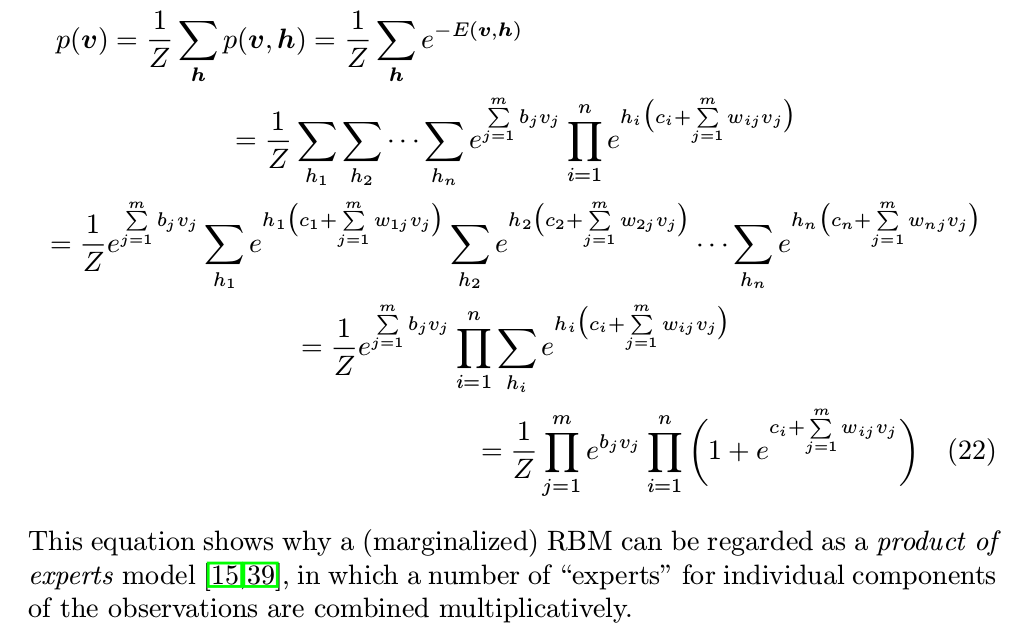
\includegraphics[scale=0.4]{formulae/prod_experts.png}
\centering
\caption{$p(\mb{v})$}
\label{fig:prod_experts}
\end{mdframed}
\end{figure}
\\[1em]
\u{Gradient of Log-Likelihood}
\\Recall
$$
\frac{\partial}{\partial\theta}\log p(\mb{v};\bs{\psi})=
-\sum_{\mb{h}}p(\mb{h}|\mb{v};\bs{\psi})\cdot\frac{\partial}{\partial\theta}E(\mb{v},\mb{h};\bs{\psi})
+\sum_{\mb{\t{v}},\mb{\t{h}}}p(\mb{\t{v}},\mb{\t{h}};\bs{\psi})\cdot\frac{\partial}{\partial\theta}E(\mb{\t{v}},\mb{\t{h}};\bs{\psi})
$$
First term for $\theta=W_{ij}$ (omit $\bs{\psi}$):
\begin{empheq}[box={\mybox[1em][1em]}]{gather*}
[1]=-\sum_{\mb{h}} \prod_kp(h_k|\mb{v}) \cdot\frac{\partial}{\partial W_{ij}}E(\mb{v},\mb{h})=\comment{$\frac{\partial}{\partial W_{ij}}E(\mb{v},\mb{h})=-v_ih_j$}=\sum_{\mb{h}} \prod_kp(h_k|\mb{v})v_ih_j=
\\=\sum_{h_j}\sum_{\mb{h}_{-j}}p(h_j|\mb{v})p(\mb{h}_{-j}|\mb{v})h_jv_i=
\sum_{h_j\in\{0,1\}}h_jp(h_j|\mb{v})v_i \underbrace{\sum_{\mb{h}_{-j}}p(\mb{h}_{-j}|\mb{v})}_{=1}=p(h_j=1|\mb{v})\cdot v_i
\end{empheq}
The second term
$$
[2]=\sum_{\mb{\t{v}},\mb{\t{h}}}p(\mb{\t{v}},\mb{\t{h}})\cdot\frac{\partial}{\partial\theta}E(\mb{\t{v}},\mb{\t{h}})=\sum_{\mb{\t{v}}}p(\mb{\t{v}})\l(\sum_{\mb{\t{h}}}p(\mb{\t{h}}|\mb{\t{v}})\cdot\frac{\partial}{\partial\theta}E(\mb{\t{v}},\mb{\t{h}})\r)
$$
and thus can be computed in the same manner.
\\Eventually we obtain the following expressions for log-likelihood gradients:
\begin{align}
\frac{\partial}{\partial W_{ij}}\log p(\mb{v};\bs{\psi}) &= p(h_j=1|\mb{v})\cdot v_i
-\sum_{\mb{\t{v}}}p(\mb{\t{v}})\cdot p(h_j=1|\mb{\t{v}})\cdot \t{v}_i
\\
\frac{\partial}{\partial b_{i}}\log p(\mb{v};\bs{\psi}) &= v_i -\sum_{\mb{\t{v}}}p(\mb{\t{v}}) \cdot \t{v}_i
\\
\frac{\partial}{\partial c_{j}}\log p(\mb{v};\bs{\psi}) &= p(h_j=1|\mb{v}) - \sum_{\mb{\t{v}}}p(\mb{\t{v}}) \cdot p(h_j=1|\mb{\t{v}})
\end{align}
+ use formulae (21), (22). Averaged over all training examples, these formulae can also be rewritten in terms of expectations. Note that $\sum_{\mb{\t{v}}} p(\mb{\t{v}})[\cdots]=\E_{\mb{\t{v}}\sim P_{\text{\text{model}}}}[\cdots]$.
\\[1em]
Despite of the sound simplification and reducing of computational complexity because of the nice factorization, (25) - (27) are still intractable for regular RBMs because of the second terms which are exponential in $\min\{V, H\}$ (if $H<V$ we can factorize $p(\mb{v},\mb{h})=p(\mb{h})p(\mb{v}|\mb{h})$).
\\[1em]Thus, to avoid this complexity, we will approximate expectations by samples from the model distribution using MCMC-based algorithm \emph{Contrastive Divergence} (described below).
\\[1em]
\u{Quick summary}
\begin{center}
\begin{tabular}{ |c|c|c| } 
\hline
& \tb{general BM} & \tb{RBM} \\
\hline
\tb{exact Maximum Likelihood learning} & \color{red}intractable & intractable$^{*}$ \\
\hline
\tb{inference} & \color{red}approximate & \color{green}exact \\
\hline
\end{tabular}
\end{center}
$^{*}$ -- learning still can be done efficiently using Contrastive Divergence.

\subsubsection{Contrastive Divergence algorithm and modifications}
All common training algorithms for RBMs approximate expectations in log-likelihood gradients (25) - (27) by only single sample from RBM and perform gradient ascent on these approximations. 
\\[1em]
Samples in RBM can be obtained by running a Markov chain to convergence, using Gibbs sampling as the transition operator. 
In general, Gibbs sampling of the joint of $N$ random variables $\bs{\xi}=(\xi_1\ldots\xi_N)$ is done through a sequence of $N$ sampling sub-steps of the form $\xi_i\sim p(\xi_i|\bs{\xi}_{-i})$. If done sequentially, one can show that these sub-steps define reversible Markov chain with desired invariant joint distribution.
\\[1em]
For RBMs, $\xi$ consists of the set of visible and hidden units. However, since they are conditionally independent, $p(v_i|\mb{h},\mb{v}_{-i})=p(v_i|\mb{h})$ and $p(h_j|\mb{v},\mb{h}_{-j})=p(h_j|\mb{v})$ one can perform \tb{block} Gibbs sampling (which is impossible in BM). In this setting, visible units are sampled simultaneously given fixed values of the hidden units. Similarly, hidden units are sampled simultaneously given the visibles. A step in the Markov chain is thus taken as follows:
\bg
\mb{h}^{(n+1)}\;\sim\;\text{Ber}(\text{sigm}\l( \mb{W}^T\mb{v}^{(n)}+\mb{c} \r)),
\\
\mb{v}^{(n+1)}\;\sim\;\text{Ber}(\text{sigm}\l( \mb{W}\mb{h}^{(n+1)}+\mb{b} \r))
\eg
Graphically:
\begin{figure}[h]
\begin{mdframed}
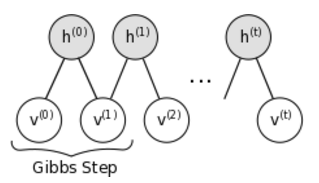
\includegraphics[scale=0.6]{img/gibbs.png}
\centering
\caption{Gibbs sampling in RBM.}
\label{fig:gibbs}
\end{mdframed}
\end{figure}
\\
As $n \rightarrow \infty$, samples $\left(\mb{v}^{(n)},\mb{h}^{(n)}\right)$ are guaranteed to be accurate samples of the model joint.
\\[1em]
In theory, each parameter update in the learning process would require running one such chain to convergence to obtain unbiased estimates of gradients of log-likelihood, which requires many sampling steps (prohibitively expensive) and moreover it is typically unclear for how long chain has to be run. As such, several algorithms have been devised for RBMs, in order to efficiently sample from.
\\[1em]
\u{Contrastive Divergence} (CD-k)
\\
This algorithm was proposed in 2002 by G.Hinton and uses two tricks to speed up the sampling process:
\begin{itemize}
\item since we eventually want $p_{\text{model}}(\mb{v}) \approx p_{\text{data}}(\mb{v})$ (Maximum Likelihood $\Leftrightarrow$ Minimizing KL divergence between $p_{\text{model}}$ and $p_{\text{data}}$ (empirical distribution)), \emph{we initialize the Markov chain with a training example}, so that the chain will be already close to having converged to its desired distribution.
\item CD does not wait for the chain to converge. Samples are obtained after only $k$-steps of Gibbs sampling. In practice, $k=1$ has been shown to work surprisingly well.
\end{itemize}
General formula for gradient approximation:
\bg
\frac{\partial}{\partial\theta}\log p(\mb{v}^{(0)};\bs{\psi})\approx 
-\sum_{\mb{h}}p(\mb{h}|\mb{v}^{(0)};\bs{\psi})\cdot\frac{\partial}{\partial\theta}E(\mb{v}^{(0)},\mb{h};\bs{\psi})
+\sum_{\mb{h}}p(\mb{h}|\mb{v}^{(k)};\bs{\psi})\cdot\frac{\partial}{\partial\theta}E(\mb{v}^{(k)},\mb{h};\bs{\psi})
\eg
Concrete formulae for gradient approximations:
\begin{align}
g_{W_{ij}} &\leftarrow p(h_j=1|\mb{v}^{(0)})\cdot v_i^{(0)}-p(h_j=1|\mb{v}^{(k)})\cdot v_i^{(k)}
\\
g_{b_i} &\leftarrow v_i^{(0)}-v_i^{(k)}
\\
g_{c_j} &\leftarrow p(h_j=1|\mb{v}^{(0)})-p(h_j=1|\mb{v}^{(k)})
\end{align}
with $\mb{v}^{(0)}:=\mb{v}$ -- training example
\\
Each gradient is a difference of the corresponding \tb{positive} and \tb{negative} gradients, see (16). It is thus described through sequence of \emph{positive phases}, where we clamp visible units to a particular state vector sampled from the training set $\mb{v}\leftarrow\mb{x}_i \sim p_{\text{data}}$, and \emph{negative phases}, where the network is run freely without fixing any states.
\\[0.5em]
\tb{Note}: originally formulae (31)-(33) should contain instead of $p(h_j=1|\mb{v})$ the samples of hidden units themselves (apart from sampling involved to estimate model's expectations), but stated variants typically provide slightly less noisy and thus faster learning, and it is not so important at all when RBM is used to pretrain hidden layer of units for DBN/DBM \cite{hinton2010practical}.
\\[1em]
Since $\mb{v}^{(k)}$ is not a sample from the stationary distribution the approximation the approximation (30) is biased. Obviously, as $k \rightarrow \infty$, bias vanishes. One can also show that CD does not maximize the likelihood of the data under the model, but minimize the difference of two KL-divergences:
\bg
D_{\text{KL}}(p_{\text{data}}(\mb{v})\;\|\;p_{\text{model}}(\mb{v}))-D_{\text{KL}}(p^{(k)}(\mb{v})\;\|\;p_{\text{model}}(\mb{v})),
\eg
where $p^{(k)}(\mb{v})$ is a distribution of visible variables after k steps of Markov chain. If chain already reached stationarity it holds that $p^{(k)}=p_{\text{model}} \;\Rightarrow\; D_{\text{KL}}(p^{(k)}(\mb{v})\;\|\;p_{\text{model}}(\mb{v}))=0$ and the approximation error of CD is vanishes.
\\[1em]
CD does not follow the gradient of any function \cite{hinton2010practical}.
\\[1em]
\u{Persistent CD}
In \cite{tieleman2008training} they rely on a single Markov chain, which has a persistent state (i.e., not restarting a chain for each observed example). For each parameter update, we extract new samples by simply running the chain for $k$-steps. The state of the chain is then preserved for subsequent updates. The general intuition is that if parameter updates are small enough compared to the mixing rate of the chain, the Markov chain should be able to "catch up" to changes in the model.
\\[1em]
Typically one uses as much markov chains as there are training examples in a minibatch. These persistent states of Markov chains can be used to generate samples after training. In \cite{hinton2010practical} they mention PCD learns significantly better models than CD-k for various k and is the recommended method if the aim is to build the best density model of the data. We will use a modification of PCD for DBM training.
\\[1em]
Also, recently the new algorithm \u{Parallel tempering} is proposed \cite{fischer2012introduction}. It introduces supplementary Gibbs chains that sample from more and more smoothed replicas of the original distribution. In the price of computational overhead it gives faster mixing Markov chain and thus less biased gradient approximation.
\subsubsection{Extensions}
\u{More general RBMs/BMs}
\\[1em]
So far we considered only case of binary (Bernoulli) both visible and hiddent units. But RBMs (and BMs) can also be extended to model $\R$-valued inputs/outputs. This can be achieved by altering the energy functio (more examples below). More generally RBM can be defined as any MRF (undirected graphical model) with conditionally independent visible units given hidden and vice versa and with energy function of the following kind:
\bg
E(\mb{v},\mb{h};\bs{\psi})=\sum_{i,j}\phi_{ij}(v_i,h_j;\bs{\psi})+\sum_i \omega_i(v_i;\bs{\psi}) + \sum_j \nu_j(h_j;\bs{\psi})
\eg
with $\R$-valued functions $\phi_{ij}, \omega_i, \nu_j$ for which partition function is finite $Z(\bs{\psi})<\infty$.
\\[1em]
\u{Conditional RBMs}
\\[1em]
some of the parameters in $E$ are replaced by parameterized functions of some conditioning random variables.
\\[1em]
\u{Classification RBMs (cRBMs)}
\\[1em]
In regular RBM we model $p(\mb{x})$. In classification RBM there are couple of choices:
\begin{itemize}
\item model $p(\mb{x},\mb{y})$ (\emph{generative mode})
\item model $p(\mb{y}|\mb{x})$ (\emph{discriminative mode}), equivalent to the above via Bayes theorem
\item $\alpha\cdot p(\mb{x},\mb{y})+(1-\alpha)\cdot p(\mb{y}|\mb{x})\rightarrow \text{max}$ (\emph{hybrid mode})
\end{itemize}
See more in \cite{hinton2010practical}.

\subsubsection{Different types of RBM units}
For a binary unit, the probability of turning on is given by the logistic sigmoid function of its total input, $x$.
\bg
p=\text{sigm}(x)=\frac{1}{1+e^{-x}}=\frac{e^x}{e^x+e^0}
\eg
The energy contributed by the unit is $-x$ if it is on and 0 if it is off. Equation (36) makes it clear that the probability of each of the two possible states is proportional to the negative exponential of its energy. This can be generalized to $K$ alternative states.
\\[1em]
\u{Softmax units}
\bg
p_j=\text{softmax}_j(\mb{x})=\frac{e^{x_j}}{\sum_{k=1}^K e^{x_k}}
\eg
It is the appropriate way to deal with a quantity that has $K$ alternative \emph{mutually exclusive} values which are not ordered in any way. When viewed in this way, the learning rule for the binary units in a softmax is identical to the rule for standard binary units.
\tb{The only difference is in the way the probabilities of the states are computed and the samples are taken} + Fig. \ref{fig:softmax_sampling}.
\\[0.5em]
Formally, for binary visible and softmax hidden: 
$$\mb{v}\in\{0,1\}^D,\mb{h}\in\text{One-hot}(H)=\l\{\mb{q}\in\{0,1\}^H \bigg| \sum_kq_k=1\r\}, H=K$$
Energy function has the same functional form, as for binary-binary RBM:
\bg
E(\mb{v},\mb{h};\bs{\psi})=-\sum_{j,l}W_{jl}v_jh_l-\sum_jb_jv_j-\sum_lc_lh_l
\eg
\\[1em]
\u{Multinomial units}
\\
Afurther generalization of the softmax unit is to sample $M$ times (with replacement) from the probability distribution instead of just sampling once. The $K$ different states can then have integer values bigger than 1, but the values must add to $M$. This is called a \emph{multinomial unit} and, again, the learning rule is unchanged. It is also equivalent \cite{hinton2009replicated} to $M$ softmax units with shared weights.
\\[0.5em]
Formally, for binary visible and multinomial hidden with $M$ samples: 
$$\mb{v}\in\{0,1\}^D,\t{\mb{h}}\in\l\{\mb{q}\in\{0,1,\ldots,M\}^H \bigg| \sum_kq_k=M\r\}, H=K$$
Energy function has the same functional form, as for binary-binary RBM:
\bg
E(\mb{v},\t{\mb{h}};\bs{\psi})=-\sum_{j,l}W_{jl}v_j\t{h}_l-\sum_jb_jv_j-\sum_lc_l\t{h}_l,
\eg
where $\t{h}_l=\sum_{m=1}^M h_l^{(m)}$ -- count for $l$-th discrete value of hidden units. Typically, this variant of RBM is used for topic modelling \cite{hinton2009replicated} (visible are Multinomial, hidden -- binary). Often $M$ is equal to $K$. In this case, it is also useful to scale hidden bias term by $M$, this will allow to behave sensible when deal with documents of the different lengths.
\\[1em]
\u{Gaussian visible units}
\\
To be able to model real-valued data $\mb{v}\in\R^D$, one solution is to replace the binary visible units by linear units with independent Gaussian noise. The energy function then becomes:
\bg
E(\mb{v},\mb{h};\bs{\psi})=\frac{1}{2}\sum_{i,j}\frac{(v_i-b_i)^2}{\sigma_i^2}-\sum_jc_jh_j-\sum_{i,j}W_{ij}\frac{v_i}{\sigma_i}h_j
\eg
where $\sigma_i$ is the standard deviation of the Gaussian noise for visible unit $i$. It is possible to learn the variance of the noise for each visible unit but this is difficult using CD-k. In many applications, it is much easier to first normalise each component of the data to have zero mean and unit variance and then to use noise free reconstructions, with the variance in equation (40) set to 1.
\\[1em]
From (38) one can derive formulae for activations \cite{salakhutdinov2013learning, krizhevsky2009learning}:
\bg
p(h_j=1|\mb{v})=\text{sigm}\l(\sum_iW_{ij}\frac{v_i}{\sigma_i}+c_j\r),
\\
v_i|\mb{h}\;\sim\;\mc{N}\l(\sigma_i\sum_jW_{ij}h_j+b_i;\;\sigma_i^2\r)=\sigma_i\sum_jW_{ij}h_j+b_i+\sigma_i\cdot\mc{N}(0; 1)
\eg
\\[1em]
There also exist other types of units, such as gaussian for both visible and hidden units, binomial units, rectifier linear units etc., but they more rarely used and are out of the scope of these notes. See more in \cite{hinton2010practical}.

\subsubsection{Free energies formulae}
\textbullet{} \u{Free energy for binary visible and hidden units (19)} (Similarly to Fig. \ref{fig:prod_experts}):
\begin{empheq}[box={\mybox[1em][1em]}]{gather*}
\mc{F}(\mb{v};\bs{\psi})=-\log\l( \sum_{\mb{h}}e^{-E(\mb{v},\mb{h};\bs{\psi})} \r)=
-\log \sum_{\mb{h}} \exp\l(\sum_{i,j}W_{ij}v_ih_j+\sum_ib_iv_i+\sum_jc_jh_j\r)=\\
=-\log \l[\exp\l(\sum_ib_iv_i\r)\cdot\sum_{\mb{h}} \exp\l(\sum_{i,j}W_{ij}v_ih_j+\sum_jc_jh_j\r)\r]=\\
=-\sum_ib_iv_i-\log \sum_{\mb{h}} \underbrace{\exp\l(\sum_jh_j\l(\sum_iW_{ij}v_i+c_j\r)\r)}_{\prod_j \exp\l(h_j\l(\sum_iW_{ij}v_i+c_j\r)\r)}=\comment{$\sum_{\mb{h}}\prod_j f_j(h_j)=\prod_j\sum_{h_j}f_j(h_j)$}=\\
=-\mb{b}\cdot\mb{v}-\sum_j \log\l( \underbrace{ \sum_{h_j\in\{0,1\}}\exp \l[h_i \sum_iW_{ij}v_i+c_j\r]}_{1+\exp\l(\sum_iW_{ij}v_i+c_j\r)}\r)
=-\mb{b}\cdot\mb{v}-\sum_j \text{softplus}\l(\sum_iW_{ij}v_i+c_j\r),
\end{empheq}
where $\text{softplus}(x):=\log(1+e^x)$.
\begin{gather}
\boxed{\mc{F}(\mb{v};\bs{\psi})=-\mb{b}\cdot\mb{v}-\sum_j \text{softplus}\l(\sum_iW_{ij}v_i+c_j\r)}
\end{gather}
\\[1em]
\textbullet{} \u{Free energy for Bernoulli-Softmax RBM (38)}:
\begin{empheq}[box={\mybox[1em][1em]}]{gather*}
\mc{F}(\mb{v};\bs{\psi})=-\log\l( \sum_{\mb{h}}e^{-E(\mb{v},\mb{h};\bs{\psi})} \r)=
-\sum_ib_iv_i-\log \sum_{\mb{h}} \underbrace{\exp\l(\sum_jh_j\l(\sum_iW_{ij}v_i+c_j\r)\r)}_{\prod_j \exp\l(h_j\l(\sum_iW_{ij}v_i+c_j\r)\r)}=\\
=-\mb{b}\cdot\mb{v}-\log \sum_{j=1}^K\exp\l(\sum_iW_{ij}v_i+c_j\r),
\end{empheq}
\begin{gather}
\boxed{\mc{F}(\mb{v};\bs{\psi})=-\mb{b}\cdot\mb{v}-\log \sum_{j=1}^K\exp\l(\sum_iW_{ij}v_i+c_j\r)}
\end{gather}
\\[1em]
\textbullet{} \u{Free energy for Bernoulli-Multinomial RBM (39)}:
\begin{empheq}[box={\mybox[1em][1em]}]{gather*}
\mc{F}(\mb{v};\bs{\psi})=-\log\l( \sum_{\t{\mb{h}}}e^{-E(\mb{v},\t{\mb{h}};\bs{\psi})} \r)=
-\sum_ib_iv_i-\log \sum_{\t{\mb{h}}} \underbrace{\exp\l(\sum_j\t{h}_j\l(\sum_iW_{ij}v_i+c_j\r)\r)}_{\prod_j \exp\l(\t{h}_j\l(\sum_iW_{ij}v_i+c_j\r)\r)}=\\
=-\mb{b}\cdot\mb{v}-\log \sum_{\t{h}_1+\ldots+\t{h}_K=M,0\leq \t{h}_l\leq M}\prod_j\exp\l(\t{h}_j\l(\sum_iW_{ij}v_i+c_j\r)\r),
\end{empheq}
For large $M$ this equation seems to be intractable to compute. But we can approximate this by sampling $\t{\mb{h}}$ from Multinomial distribution with equiprobable states and applying appropriate scaling, note that
$$
\l | \l\{\mb{q}\in\{0,1,\ldots,M\}^H \bigg| \sum_kq_k=M\r\} \r |=\#_{M,K}=\binom{M+K-1}{K-1}=\frac{\Gamma(M+K)}{\Gamma(M+1)\Gamma(K)}
$$
So
\begin{empheq}[box={\mybox[1em][1em]}]{gather*}
\t{\mb{h}}\;\sim\;\text{Multinomial}\l(\mb{p}=\l(\frac{1}{K}\ldots\frac{1}{K}\r); M\r),
\\
\mc{F}(\mb{v};\bs{\psi}) \approx -\mb{b}\cdot\mb{v}-\log \l(\frac{\Gamma(M+K)}{\Gamma(M+1)\Gamma(K)}\r)-\sum_j \t{h}_j \l(\sum_iW_{ij}v_i+c_j\r)
\end{empheq}
\begin{gather}
\boxed{ \mc{F}(\mb{v};\bs{\psi})\approx -\mb{b}\cdot\mb{v}-\texttt{lgamma}(M+K)+\texttt{lgamma}(M+1)+\texttt{lgamma}(K)-\sum_j \t{h}_j \l(\sum_iW_{ij}v_i+c_j\r) }
\end{gather}
\\[1em]
\textbullet{} \u{Free energy for Gaussian-Bernoulli RBM}:
\\Derivation is straightforward, the formula is very similar to (43), but with accordingly changed bias term for visible units, and scaled visible units by their resp. std. deviation:
\begin{gather}
\boxed{\mc{F}(\mb{v};\bs{\psi})=\frac{1}{2}\l\|\frac{\mb{v}-\mb{b}}{\bs{\sigma}}\r\|^2-\sum_j \text{softplus}\l(\sum_iW_{ij}\frac{v_i}{\sigma_i}+c_j\r)}
\end{gather}
or equivalently if $\t{\mb{v}}\leftarrow \mb{v}/\bs{\sigma}$ (element-wise division, and also in (46),(47)):
\begin{gather}
\boxed{\mc{F}(\mb{v};\bs{\psi})=\frac{1}{2}\l\|\t{\mb{v}}-\frac{\mb{b}}{\bs{\sigma}}\r\|^2-\sum_j \text{softplus}\l(\sum_iW_{ij}\t{v_i}+c_j\r)}
\end{gather}

	\newpage
\section{Practical aspects, implementation and experiments (RBM) \cite{coursera_nn, tutorial2014lisa, hinton2010practical, yosinski2012visually, goodfellow2016deep}}
If not states otherwise, Bernoulli-Bernoulli RBM is assumed.
\subsection{How to debug/track progress}
RBMs are particularly tricky to train. Because of the partition function $Z$ we cannot estimate the log-likelihood $\log p(\mb{v})$ directly during training. We therefore have no direct useful metric for choosing the optimal hyperparameters.

\subsubsection{Inspection of Negative particles}
Negative samples (samples used to estimate negative phase of the log-likelihood gradient) obtained during training can be visualized. As training progresses, we know that the model defined by the RBM becomes closer to the true underlying distribution. For example, see Fig. \ref{fig:rbm_samples}.
\begin{figure}[h]
\begin{mdframed}
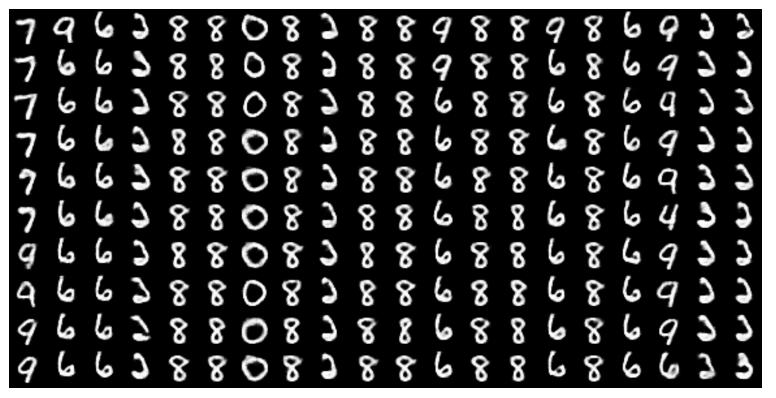
\includegraphics[scale=0.4]{img/rbm_samples.png}
\centering
\caption{Samples generated by the RBM after PCD-15 training on MNIST. Each row represents a mini-batch of negative particles (samples from independent Gibbs chains). 1000 steps of Gibbs sampling were taken between each of those rows.}
\label{fig:rbm_samples}
\end{mdframed}
\end{figure}

\subsubsection{Visual Inspection of Filters}
The filters learnt by the model can be visualized. This amounts to plotting the weights of each unit as a gray-scale image (after reshaping to a square matrix). Filters should pick out strong features in the data. While it is not clear for an arbitrary dataset, what these features should look like, training on MNIST usually results in filters which act as stroke detectors, while training on natural images lead to Gabor like filters if trained in conjunction with a \tb{sparsity criteria} (more details in next subsections). For example, see Fig. \ref{fig:rbm_filters}. It is worth noting that filters may or may not be \emph{sparse}. If filters are sparse, they will respond to very local features. Dense filters, on the other hand, respond to stimuli across the entire filter. Although the two types
of filter are qualitatively different, in \cite{yosinski2012visually} they observed cases in which both types are successful in learning the underlying density.
\begin{figure}[h]
\begin{mdframed}
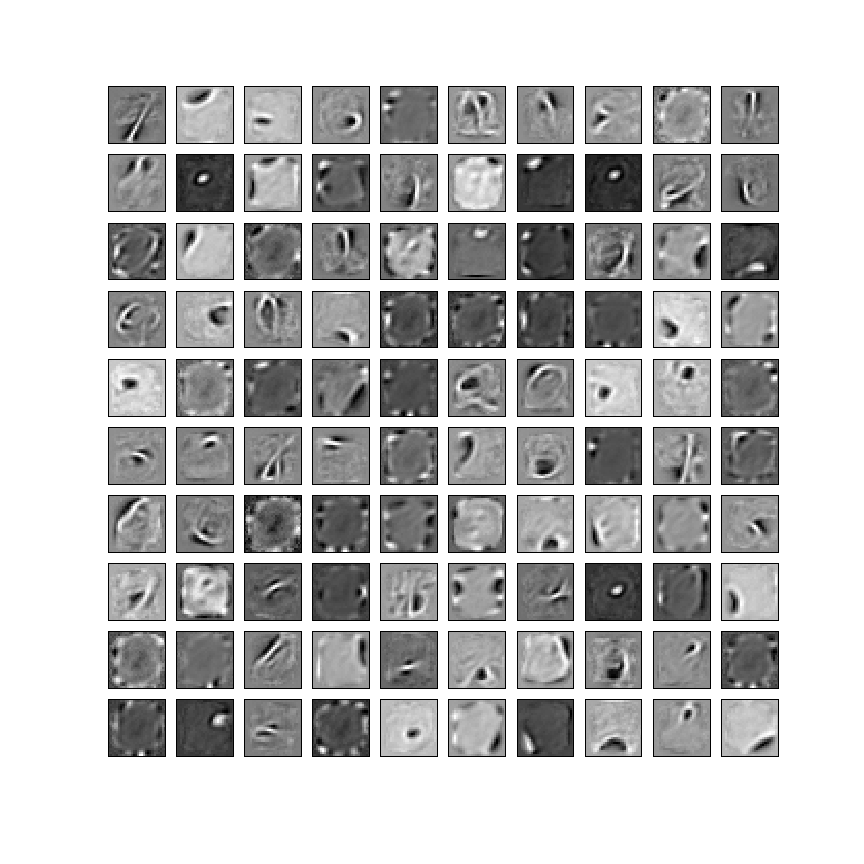
\includegraphics[scale=0.4]{rbm-mnist/rbm_filters.png}
\centering
\caption{Filters learned by RBM after CD-1 training on MNIST.}
\label{fig:rbm_filters}
\end{mdframed}
\end{figure}

\subsubsection{Probabilities of hidden activations}
It is useful to plot activations of hidden neurons to see how they are being used, how often they are likely to be on vs. off, are there any "dead" neurons (which are always on of always off) etc. This can be effectively done by plotting greyscale matrix of probabilities of (some) hidden units for each of the input example in a minibatch, for instance. For example, see Fig. \ref{fig:rbm_hidden_activations}.
\begin{figure}[h]
\begin{mdframed}
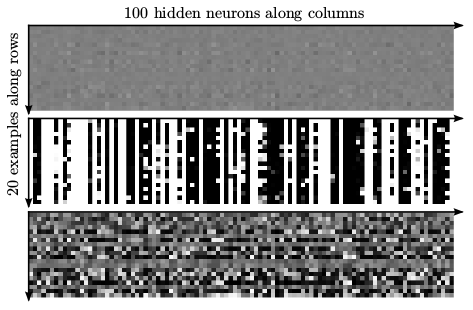
\includegraphics[scale=0.64]{img/rbm_hidden_activations.png}
\centering
\caption{Hidden neuron activation probabilities for the first 100 neurons (of 1,000) and the first 20 example data points (of 50,000), where black represents p = 0 and white, p = 1. Each row shows different neurons’ activations for a given input example, and each column shows a given neuron’s activations across many examples. Top: correct dithered gray before training begins. Values are mostly in [.4, .6]. Middle: Values pegged to black or white after one mini-batch. Decrease initial $\mb{W}$ values or learning rate. Bottom: the learning has converged well after 45 epochs of
training.}
\label{fig:rbm_hidden_activations}
\end{mdframed}
\end{figure}
\\[1em]Before any training, the probability plot should be mostly a flat gray, perhaps with a little visible noise. That is, most hidden probabilities should be around .5, with some as low as .4 or as high as .6. If the plot is all black (near 0) or all white (near 1), the weights or hidden biases were set incorrectly. The weights $\mb{W}$ should initially be random and centered at 0, and hidden biases should be zero or at least centered at zero. If the probability plot contains both pixels pegged to black and pixels pegged to white, then the $\mb{W}$ has been initialized with values too large. Intuitively, the problem with this case is that all hidden neurons have already determined what features they are looking for before seeing any of the data. 
\\
\tb{TL;DR:} when learning is working properly, this display should look thoroughly random w/o any obvious vertical or horizontal lines.

\subsubsection{Distribution/histograms of weights and weights updates}
In addition to the hidden probability plots above, it is often useful to monitor distributions of the model parameters (weights and biases) themselves, and their corresponding parameters \tb{updates} (for vanilla SGA (stoch. gradient ascent) they are gradient$\times$learning rate, and slightly more complicated formulae when using momentum or others more advanced variants of SGA). Under normal, desired conditions in the middle of
training, all histograms should look roughly Gaussian in shape, and the mean magnitudes of parameters updates should be smaller by a factor of $10^2$ to $10^4$ than mean magnitudes of the respective parameters. If the change in weights is too small (i.e. a separation of more than
$10^4$), then the learning rate can probably be increased. If the change in weights is too large, the learning may explode and the weights diverge to infinity.

\subsubsection{Proxies to Likelihood}
Other, more tractable functions can be used as a proxy to the likelihood. When training an RBM with CD/PCD, one can use \tb{pseudo-likelihood} as the proxy. Pseudo-likelihood (PL) is much less expensive to compute, as it assumes that all bits are independent
\bg
\text{PL}(\mb{v})=\prod_{i=1}^D p(v_i|\mb{v}_{-i}), \text{ and}
\\
\text{PLL}(\mb{v}):=\log \text{PL}(\mb{v})=\sum_{i=1}^D \log p(v_i|\mb{v}_{-i})
\eg
[  Compare to $\log p(\mb{v})=\log p(v_1)+\log p(v_2|v_1) +\ldots + \log p(v_D|\mb{v}_{1:D-1})$  ].
\\[1em]
For general probabilistic graphical model, $\log p(v_i|\mb{v}_{-i})=\log p(v_i|\mb{v}_{\mc{N}(i)})$, where $\mc{N}(i)$ -- set of neighbors of variable $i$. One can show that estimation by maximizing the pseudolikelihood is asymptotically consistent \cite{goodfellow2016deep}.
\\[1em]
\u{Lets calculate $p(v_i=1|\mb{v}_{-i})$ for RBM} (omit $\bs{\psi}$ for brevity)
\begin{empheq}[box={\mybox[1em][1em]}]{gather*}
p(v_i=1|\mb{v}_{-i})=\frac{p(v_i=1,\mb{v}_{-i})}{p(\mb{v}_{-i})}=\frac{p(v_i=1,\mb{v}_{-i})}{p(v_i=1,\mb{v}_{-i})+p(v_i=0,\mb{v}_{-i})}=
\frac{\frac{1}{Z}e^{-\mc{F}(v_i=1,\mb{v}_{-i})}}{\frac{1}{Z}e^{-\mc{F}(v_i=1,\mb{v}_{-i})} + \frac{1}{Z}e^{-\mc{F}(v_i=0,\mb{v}_{-i})}}=
\\=\frac{e^{-\mc{F}(v_i=1,\mb{v}_{-i})}}{e^{-\mc{F}(v_i=1,\mb{v}_{-i})} + e^{-\mc{F}(v_i=0,\mb{v}_{-i})}}=\frac{1}{1 + e^{-\l[\mc{F}(v_i=0,\mb{v}_{-i})-\mc{F}(v_i=1,\mb{v}_{-i})\r]}}=\text{sigm}\l[\mc{F}(v_i=0,\mb{v}_{-i})-\mc{F}(v_i=1,\mb{v}_{-i})\r]
\end{empheq}
So:
\begin{gather}
\boxed{p(v_i=1|\mb{v}_{-i})=\text{sigm}\l[\mc{F}(v_i=0,\mb{v}_{-i})-\mc{F}(v_i=1,\mb{v}_{-i}) \r)}
\end{gather}
Note how this formula (and derivation) resembles formulae (11),(12). This is because free energy is designed as $p(\mb{v})\;\propto \;e^{-\mc{F}(\mb{v})}=:p^*(\mb{v})$, similarly to $p(\mb{v},\mb{h})\;\propto \;e^{-E(\mb{v},\mb{h})}=:p^*(\mb{v},\mb{h})$. We also reduced complexity to only $O(V)$ invocations of unnormalized probability $p^*(\mb{v})$ instead of $O(2^{V+H})$ invocations of $p^*(\mb{v},\mb{h})$ to compute partition function for true log-likelihood.
Using equations (49),(50),(43), we can now compute PLL, which is the sum of the log-probabilities of each bit/feature $v_i$, conditioned on the state of all other bits. For moderate $D$ (e.g. for MNIST $D=784$), this sum remains rather expensive. For this reason, the following stochastic approximation to PLL is often used \cite{tutorial2014lisa, scikit-learn}:
\bg
\boxed{  \t{\text{PLL}}(\mb{v})=D\cdot \log \text{sigm}\l( \mc{F}(\t{\mb{v}}_{\tau})-\mc{F}(\mb{v}) \r), \;\;\tau \sim U(\{1\ldots D\})  },
\eg
where $\t{\mb{v}}_{i}$ is $\mb{v}$ with $i$-th bit flipped (0 $\rightarrow$ 1, 1 $\rightarrow$ 0).\\
\tb{Note}: $\E_{\tau}[\t{\text{PLL}}(\mb{v})]=\text{PLL}(\mb{v})$.
\\
\tb{Note}: Do not compute $\log \text{sigm}(x)$ naively, it is numerically unstable operation. Either observe that $\log \text{sigm}(x)=-\text{softplus}(-x)$ and use numerically stable implementation of softplus or use built-in functions (e.g. \texttt{tf.log\_logistic} in TensorFlow $\geq$ 1.2).
\\[1em]
This stochastic approximation uses only $2=O(1)$ invocations of $p^*(\mb{v})$/free-energy \tb{per training example}. Note that typically one compute average free-energy over all (or subset of) training set.
\\[1em]
\tb{Note} Some also monitor \emph{reconstruction error} during training. Although it is convenient, it is poor measure of actual RBM performance, since this is not the function Contrastive Divergence optimizes. However, typically, nicely trained model has low reconstruction error.
\\[1em]
Also there is Markov-chain based method to estimate partition function of RBM called \emph{Annealed Importance Sampling} \cite{salakhutdinov2013learning}, which can be used to estimate log-probabilities of validation data directly. We will use this methods for DBMs.

\subsubsection{Monitoring overfitting: Free energy gap}
Unfortunately, for large RBMs, it is very difficult to compute this probability
because it requires knowledge of the partition function. Nevertheless, it is possible to directly monitor
the overfitting by comparing the free energies of training data and held out validation data. In this
comparison, the partition function cancels out. As we saw, the free energy of a data vector can be computed in
a time that is linear in the number of hidden units. As the
model starts to overfit the average free energy of the validation data will rise relative to the average
free energy of the training data and this \emph{gap} represents the amount of overfitting. (Since $p(\mb{v})\propto e^{-\mc{F}(\mb{v})}$ this means network will put noticeably higher probability to training data). Free energy can be computed for subset of training (and validation data), but the same subsets should be used for the whole training.

\subsection{Choice of hyperparameters, various tricks to improve/speedup learning}
Most of the tricks and recipes are taken from \cite{hinton2010practical}.

\subsubsection{Number of Gibbs steps}
In theory the more steps we use to estimate model expectations, the better approximation of gradients we should obtain, and better learning should be observed.
\\[0.5em]
\bad However, in my experiments on MNIST, more steps decrease performance for both RBM and DBM in terms of both pseudo-loglik and quality of filters and samples.
\\
\textbullet{} In \cite{hinton2010practical} they suggest to gradually increase $k$ in CD-k during training. This is not currently implemented.

\subsubsection{Updating hidden and visible states}
The question can we or should we use probabilities instead of samples in update rules of contrastive divergence (31)-(33). It is very important to make hidden units driven by data stochastic -- this will act as a strong regularizer (network won't be able to communicate real values to the hidden units -- information bottleneck). Further updates of hidden units and all updates of visible units should use probabilities instead of sampling for less noisy and faster learning.
\\[0.5em]
\bad In the experiments if data-driven hidden units were sampled and for the rest probabilities were used, this model had the lowest pseudo-likelihood and sharp filters, see Fig. \ref{fig:rbm_sampling}. This is typically means overfitting
\\
\textbullet{} If probabilities were used only for visible units, this model had the highest PLL, but still some of the filters were sharp. This model is best suited for supervised tasks (e.g. finetuning using backprop for classification)
\\
\textbullet{} If both hidden and visible units are sampled when estimating model statistics, the learned filters are smooth and large number of them are sparse. This model has slightly worse PLL, thus we observe underfitting. When RBMs are trained to learn compound models, such as DBMs/DBNs, generative model is not the ultimate objective and it may be possible to save time by underfitting it.
\\
\good Data-driven hidden states should absolutely be sampled.
\begin{figure}[h]
\begin{mdframed}
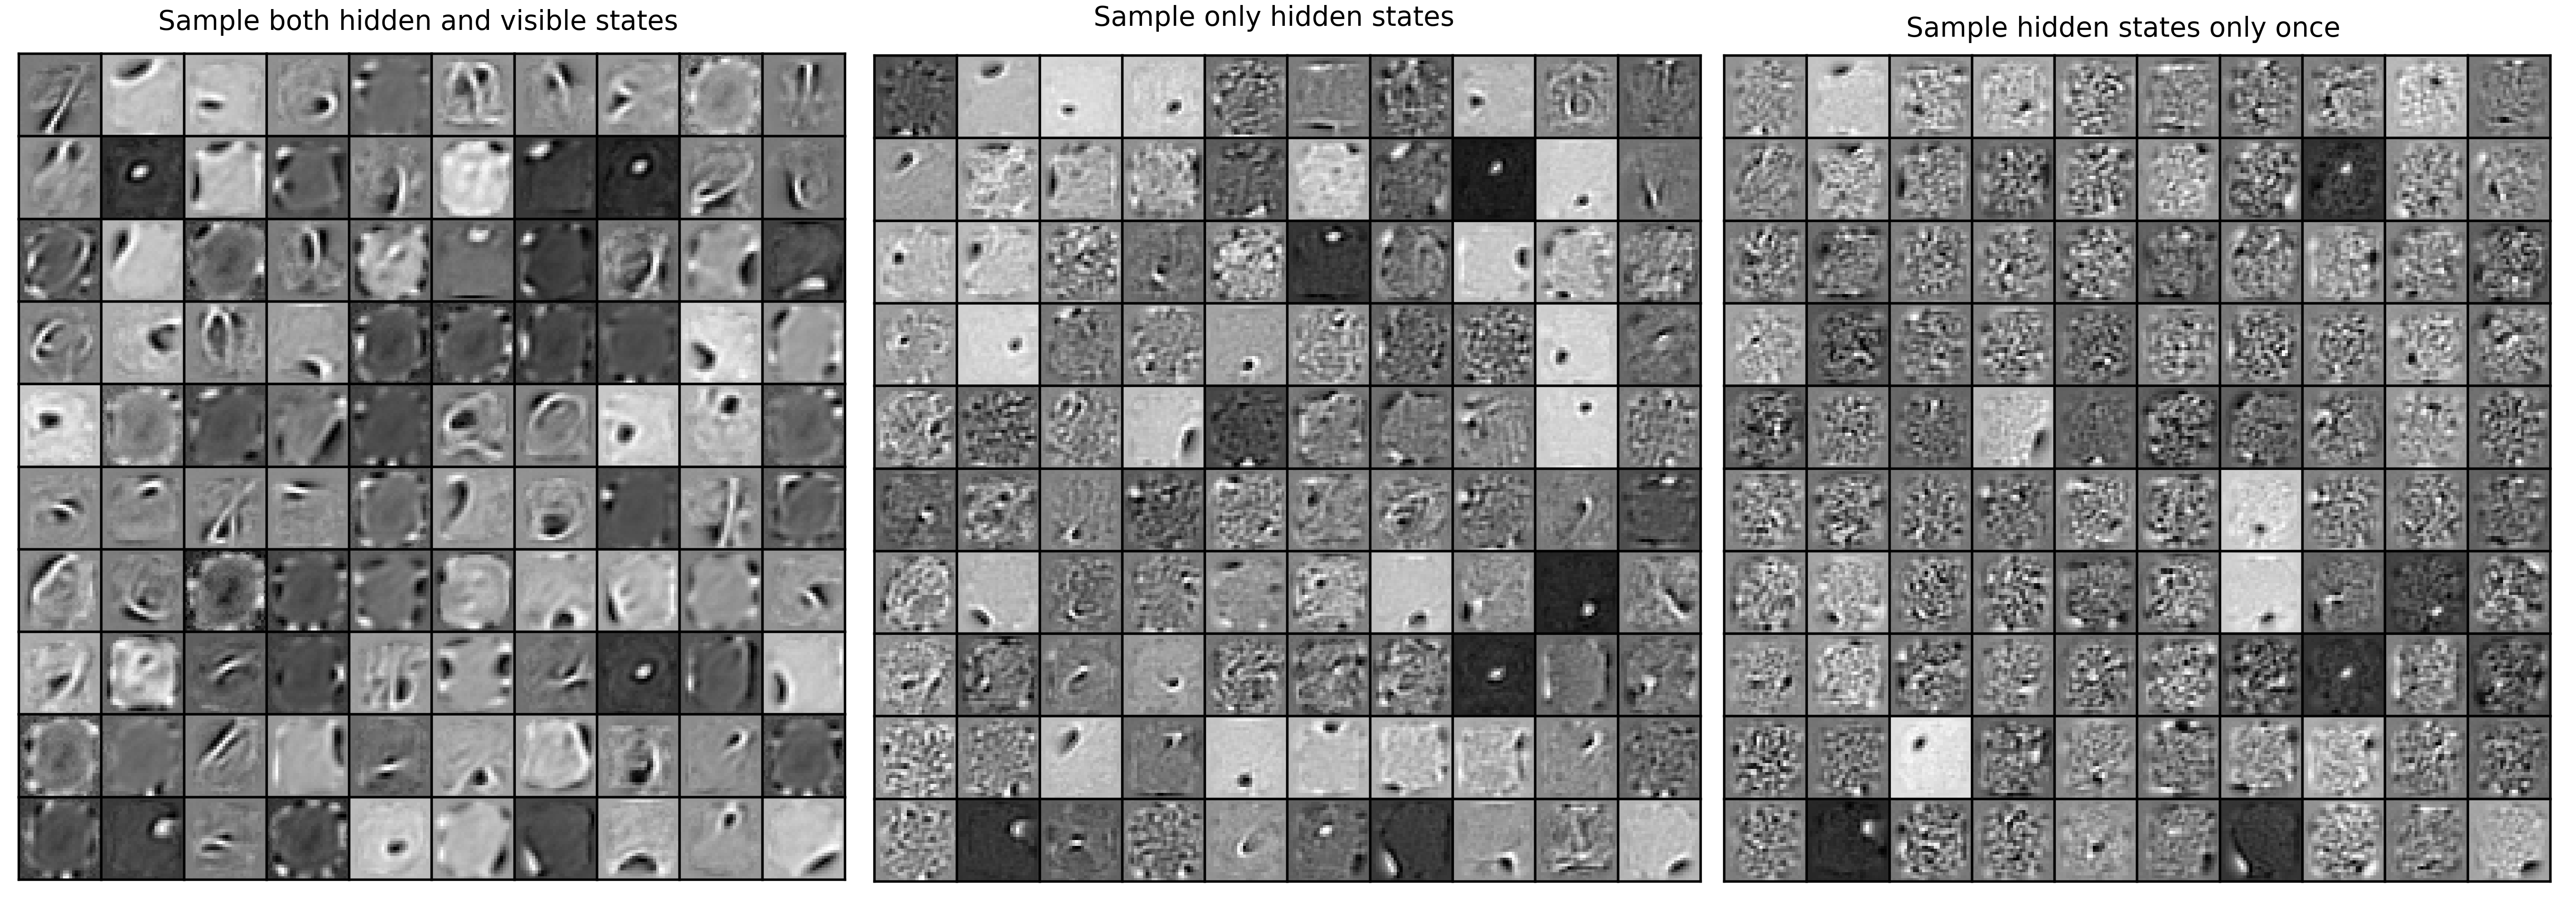
\includegraphics[scale=0.17]{rbm-mnist/rbm_sampling.png}
\centering
\caption{RBM filters trained on MNIST depending on whether to sample hidden and/or visible units.}
\label{fig:rbm_sampling}
\end{mdframed}
\end{figure}

\subsubsection{Minibatch size}
\good It is a serious mistake to make batchsizes too large. Batch size of 1 is ok, but more efficient 10-100 for more efficient computations using linalg libraries. For datasets that contain a small number of equiprobable classes, the ideal mini-batch size is often
equal to the number of classes and each mini-batch should contain one example of each class.

\subsubsection{Learning rate}
\good Shouldn't be too high (weights could explode) and not too low (slow learning). Typically it should be from $10^{-4}$ to $10^{-2}$ of order of magnitude of weights (check histogram).
\\
\good For Gaussian visible units the learning rate needs to be about one or two orders of magnitude smaller than when using binary visible units.
\\
\textbullet{} For larger $k$ in CD-k and in case of Persistent CD-k it is reasonable to slightly reduce learning rate.

\subsubsection{Initial values of the weights and biases}
\good weights are typically initialized to small zero-centered Gaussian random variables with std of about 0.01 (too large could speedup learning but also can cause "died" units (with either too large or too small activation probabilities), which slows learning).
\\
\textbullet{} weights can also be initialized to zeros, but only if hidden states are sampled (this way they still will be different even if they initially had identical connectivities)
\\
\good it is usually helpful to initialize the bias of visible unit $i$ to $\log[p_i/(1-p_i)]=\text{sigm}^{-1}(p_i)$, where $p_i$ is the proportion of training vectors in which unit $i$ is on. This will ensure that in early stages of training visible units will have activation probabilities close to $p_i$. Models with such initialization had noticeably higher PLL on MNIST.
\\
\textbullet{} $\log[t/(1-t)]=\text{sigm}^{-1}(t)$ for hidden units if sparsity target $t$ is used, otherwise zero.
\\
\bad Do not initialize hidden biases to large negative values, like $-4$ to crudely encourage sparsity. Such models had lower PLL and worse filters.

\subsubsection{Momentum method}
\good Using momentum dramatically speedups learning. In \cite{hinton2010practical} and \cite{dbm_code} they suggest to start with 0.5 and after couple of epochs to instantly increase momentum to 0.9. I found that gradually increasing momentum from 0.5 to 0.9 is slightly better. Common constant schedules for momentum, like 0.9 are also fine.

\subsubsection{Weight decay}
\good It definitely helps, and there are multiple reasons to use weight decay (not only to prevent overfitting!):
\begin{itemize}
	\item to improve generalization by preventing overfitting
	\item "unstick" hidden units that were either firmly "on" or "off"
	\item improve mixing rate of Gibbs chain which makes CD better approximate log-likelihood gradients etc.
\end{itemize}
Good values for weight decay coefficient are $10^{-5}\ldots10^{-2}$.

\subsubsection{Different regularization techniques}
\textbullet{} L1 weight-decay often leads to strongly localized receptive fields (many of the weights to become exactly zero whilst allowing a few of the weights to grow quite large, this can make it easier to interpret the weights).
\\
\textbullet{} Maxnorm helps to avoid hidden units getting stuck with extremely small weights, but a sparsity target is probably a better way to avoid this problem. Maxnorm will play more important role in DBM training, though.
\\
\textbullet{} Dropout: does not seem to help in any way.  

\subsubsection{Encouraging sparse hidden activities: sparsity targets}
Sparse activities of the binary hidden units can be achieved by specifying a "sparsity target" which is the desired probability of being active, $t<<1$ (typically $t=0.01$ to $t=0.1$. An additional penalty term is then used to encourage the actual probability of being active $q$ to be close to $t$. $q$ is estimated by using an exponentially decaying average of the mean probability that a unit is active in each mini-batch:
\bg
q \leftarrow \omega q + (1-\omega) q_{\text{current}},
\eg
where $q_{\text{current}}$ is the mean activation probability of the hidden unit on the current mini-batch, decay rate $\omega$ is typically 0.9 to 0.99. For logistic hidden units the natural penalty measure to use is the cross entropy between the desired and actual distributions:
\bg
\text{Sparsity penalty}=\lambda\times\l[ -t\log q-(1-t)\log(1-q) \r],
\eg
where $\lambda$ is a hyperparameter called "sparsity cost". (53) has simple derivative of $\lambda (q-t)$ w.r.t. total input of a unit. It is imprtant to apply the same derivative to both weights and hidden biases. Histogram the mean activities of the hidden units and set the sparsity-cost so that the hidden units have mean probabilities in the vicinity of the target. If the probabilities are tightly clustered around the target value, reduce the sparsity-cost so that it interferes less with the main objective of the learning.

\subsubsection{Number of hidden units}
\good It is common and useful to use more hidden units than visible, especially in conjunction with a sparsity target. (In discriminative learning labels usually contain very few bits of information, so using more parameters than training cases will typically cause severe overfitting; when learning generative models of high-dimensional data, however, it is the number of bits that it takes to specify a data vector that determines how much constraint each training case imposes on the parameters of the model. This can be several orders of magnitude greater than number of bits required to specify a label.)

\subsection{Experiments}
Also check jupyter notebooks in github repo. All RBMs here are trained on MNIST.

\begin{figure*}[t!]
\begin{mdframed}
\centering
\begin{subfigure}[t]{0.5\textwidth}
    \centering
    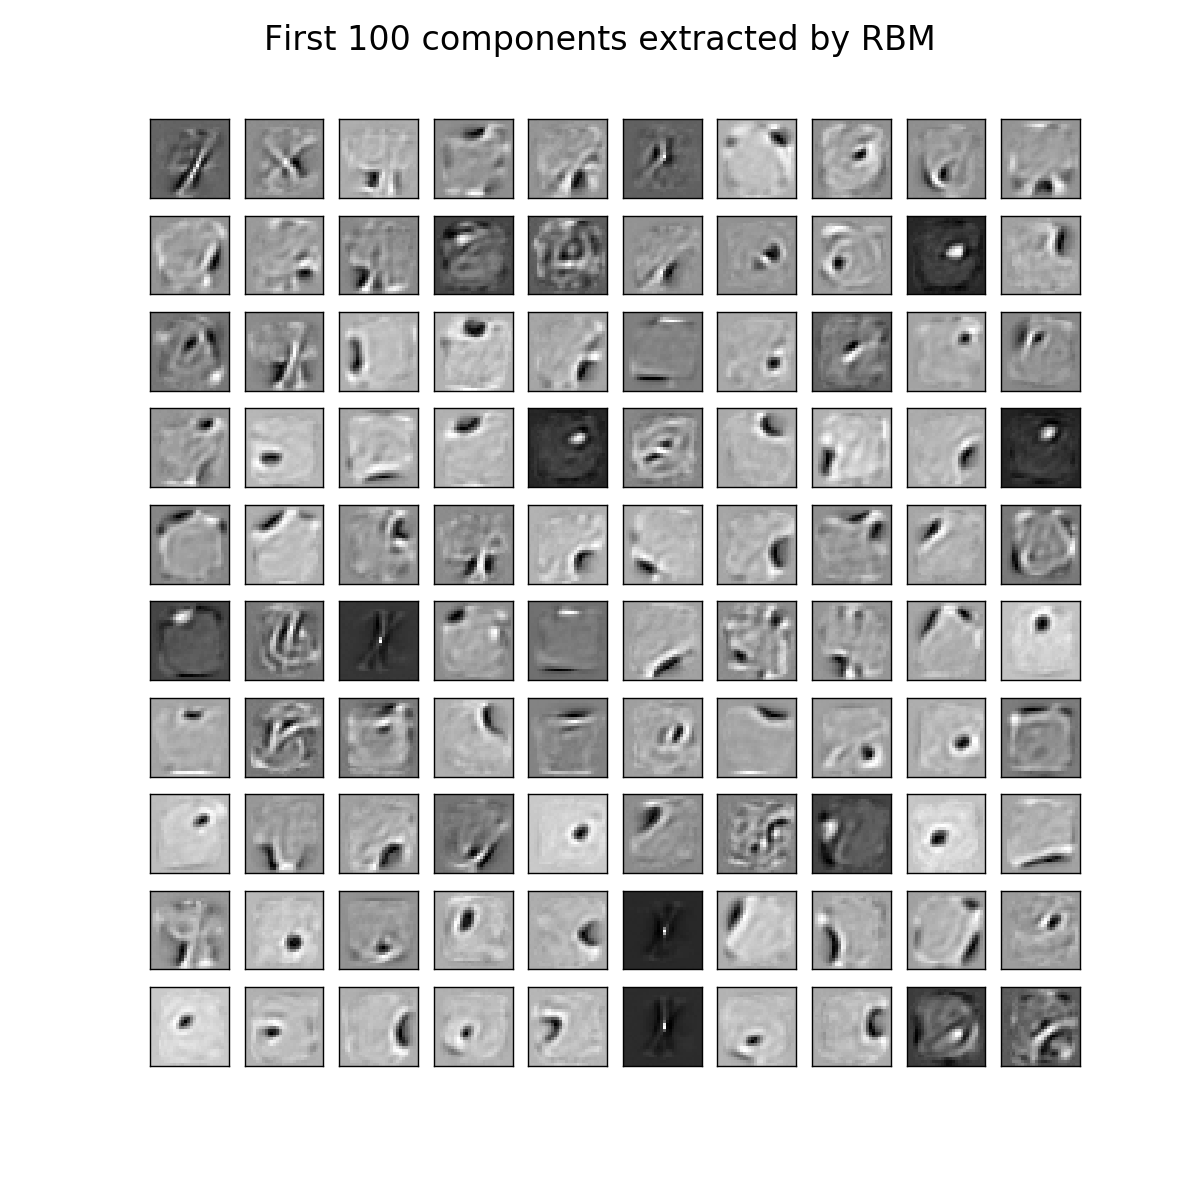
\includegraphics[height=3.2in]{rbm-mnist/rbm_mnist_256.png}
    \caption{256 hidden layers}
\end{subfigure}%
~
\begin{subfigure}[t]{0.5\textwidth}
    \centering
    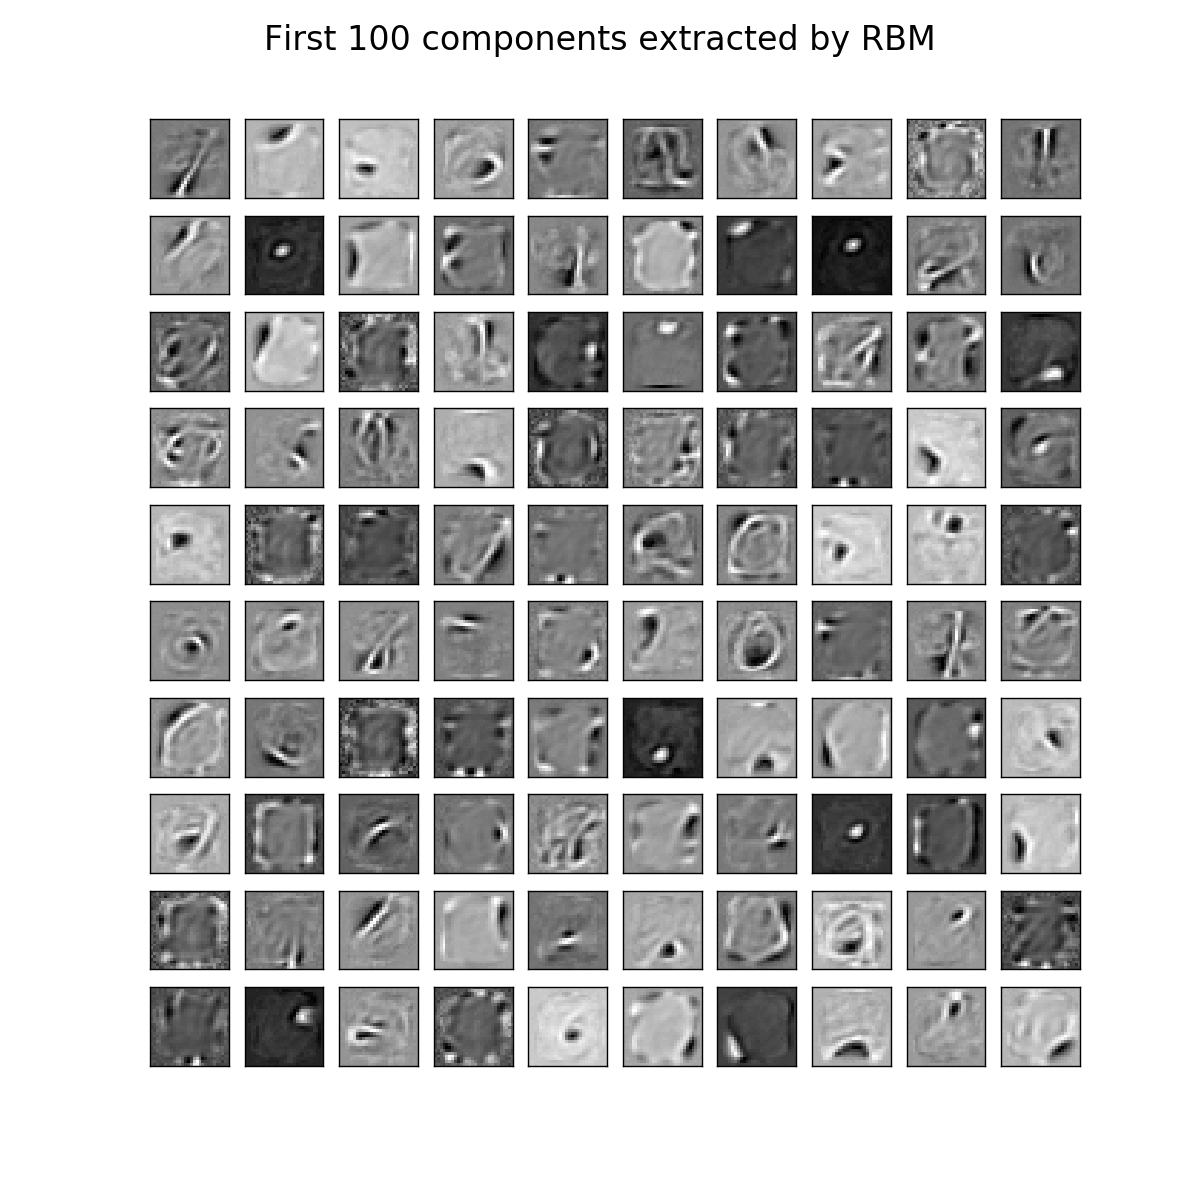
\includegraphics[height=3.2in]{rbm-mnist/rbm_mnist_1024.png}
    \caption{1024 hidden layers}
\end{subfigure}
\caption{Different number of hidden layers}
\end{mdframed}
\end{figure*}

\begin{figure}[h]
\begin{mdframed}
\centering
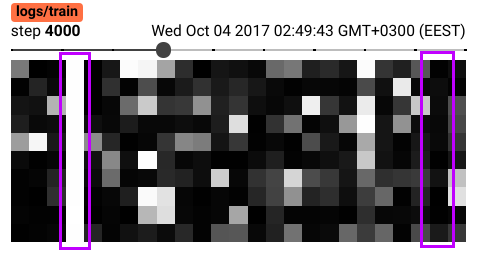
\includegraphics[width=4.2in]{rbm-mnist/dropout.png}
\caption{Dropout $p=0.9$ kills some hidden units.}
\end{mdframed}
\end{figure}

\clearpage

\begin{figure}[h]
\begin{mdframed}
\centering
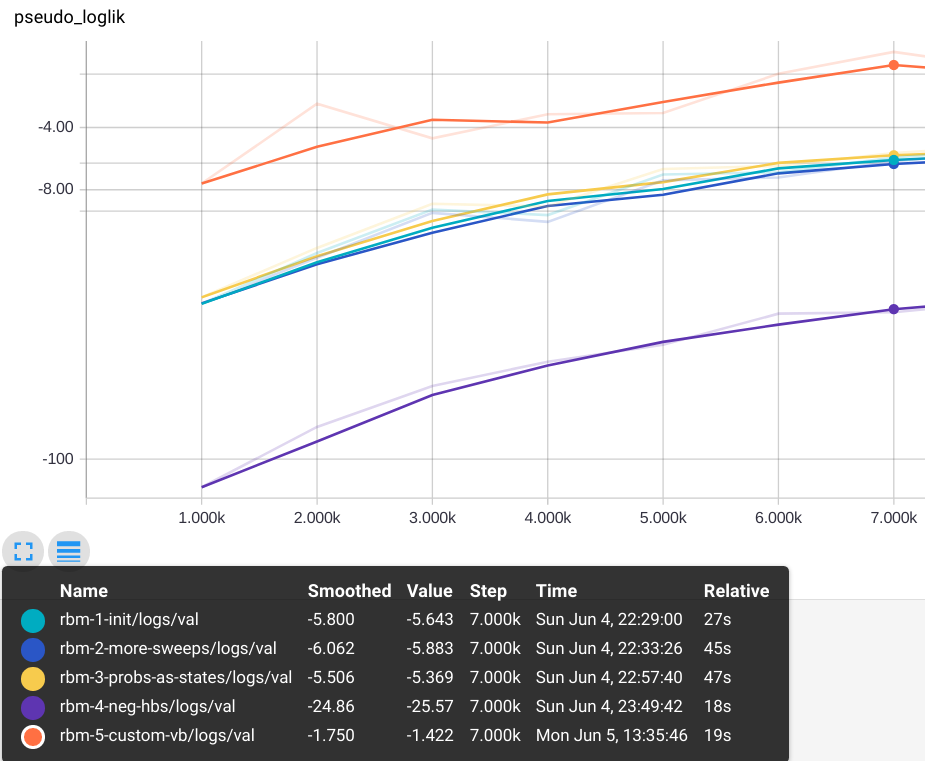
\includegraphics[width=4.8in]{rbm-mnist/rbm-runs_10k.png}
\\[2em]
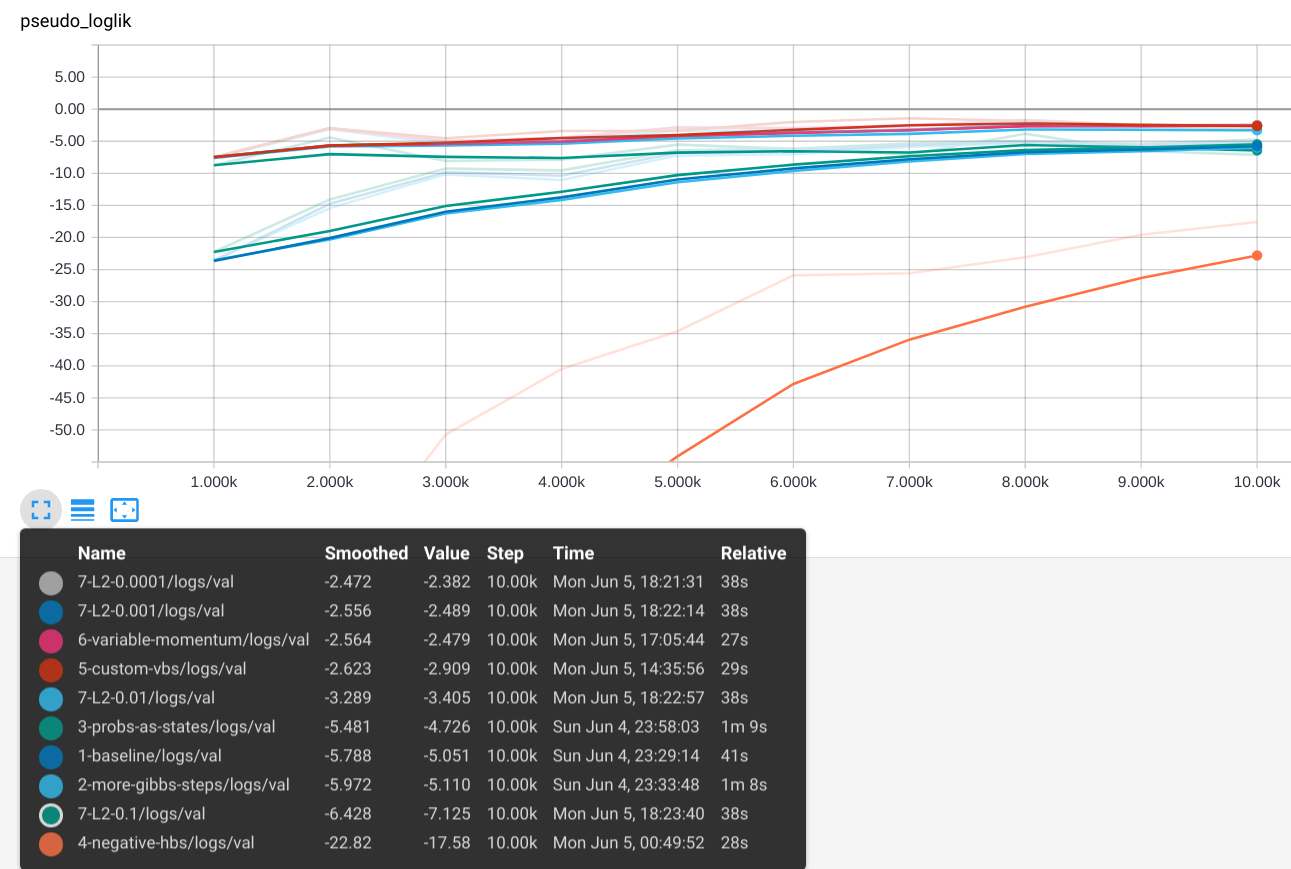
\includegraphics[width=4.8in]{rbm-mnist/rbm_practical_10k.png}
\caption{PLL of RBMs trained using various approaches on 10k MNIST digits.}
\end{mdframed}
\end{figure}

\clearpage

\begin{figure*}[t!]
\begin{mdframed}
\centering
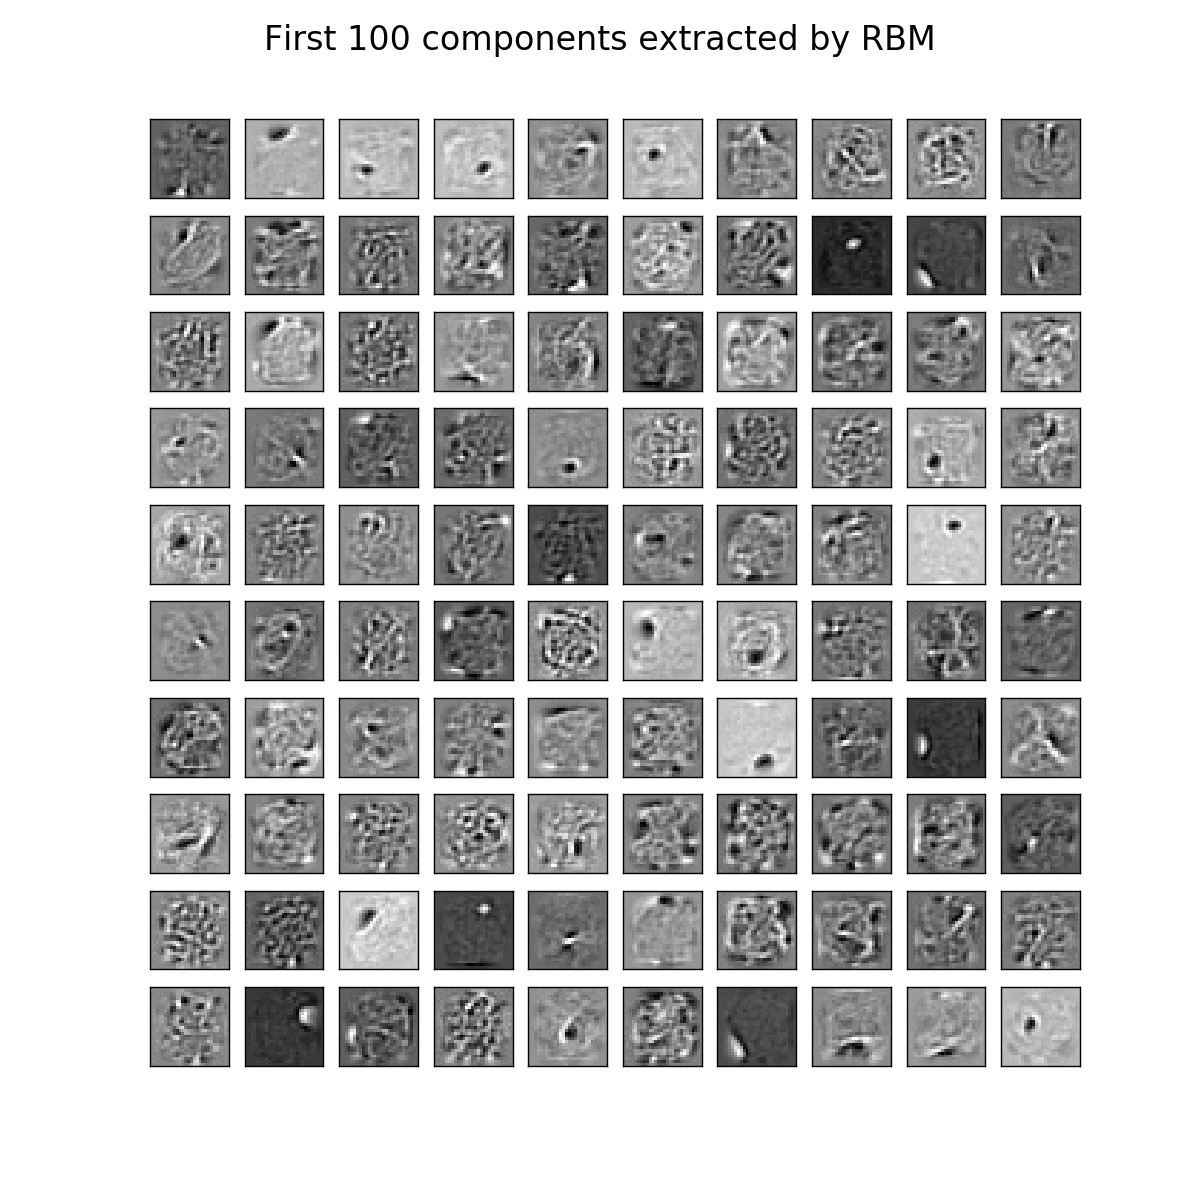
\includegraphics[width=.31\textwidth]{rbm-mnist/L1e-5.png}\quad
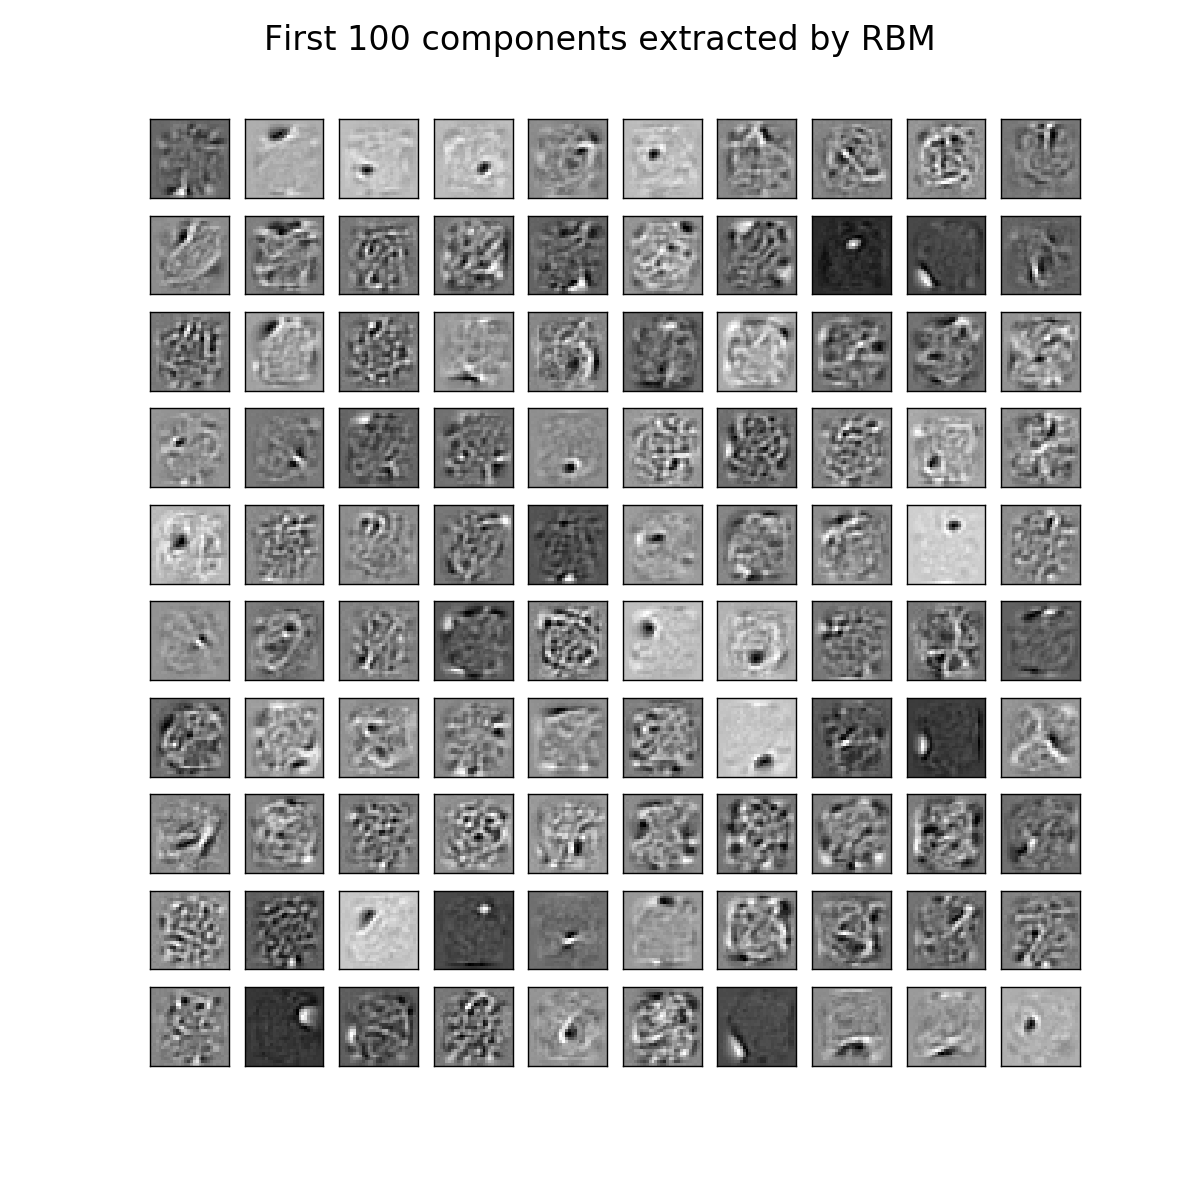
\includegraphics[width=.31\textwidth]{rbm-mnist/L1e-4.png}\quad
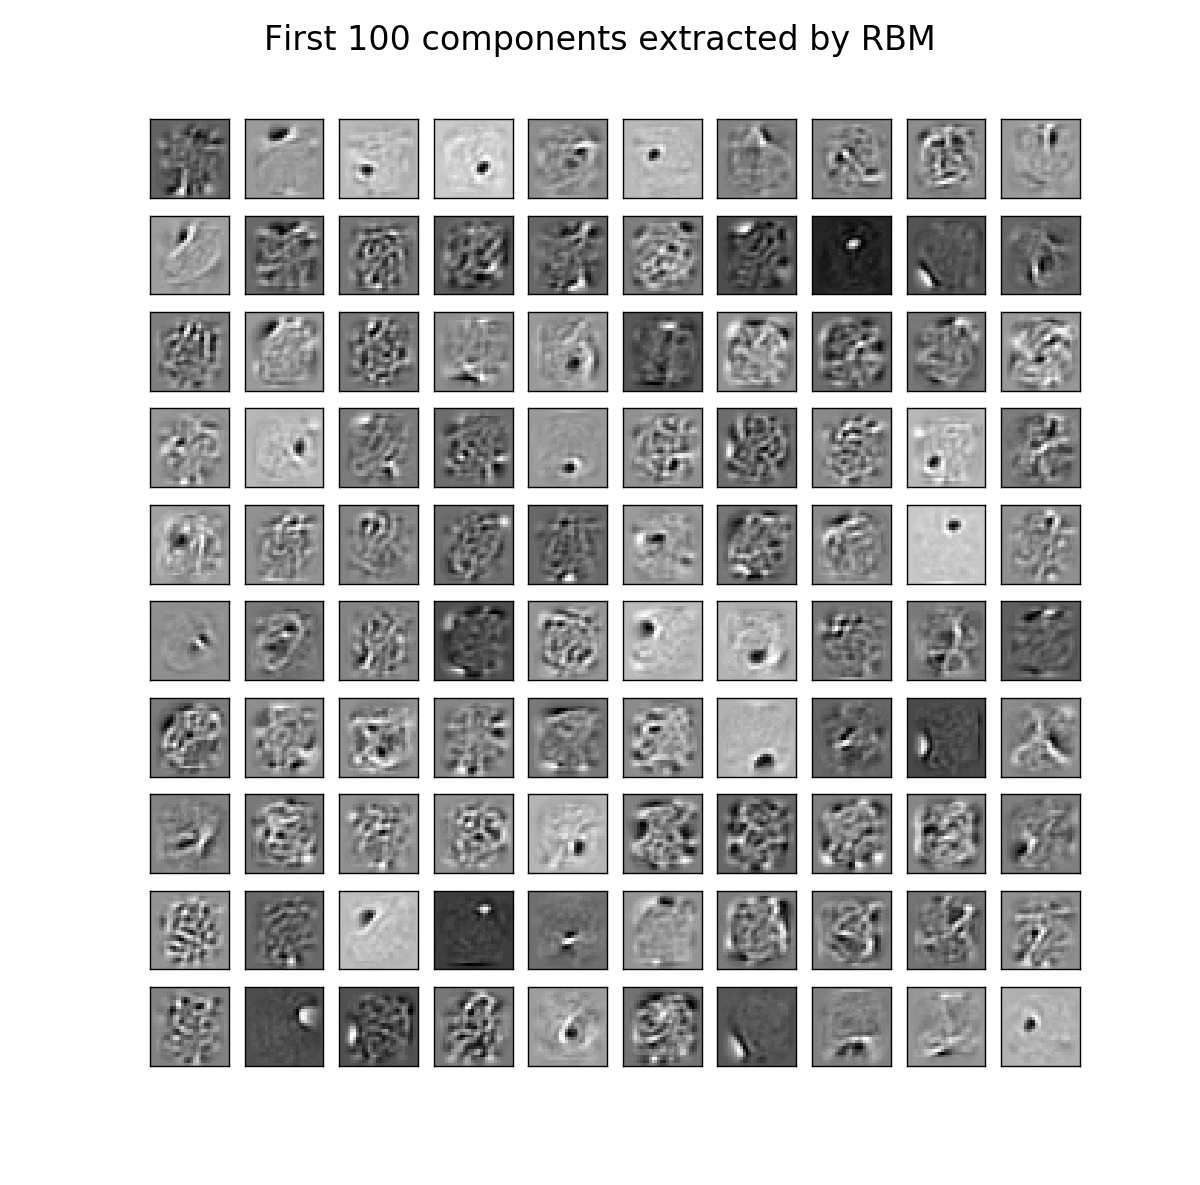
\includegraphics[width=.31\textwidth]{rbm-mnist/L1e-3.png}

\medskip

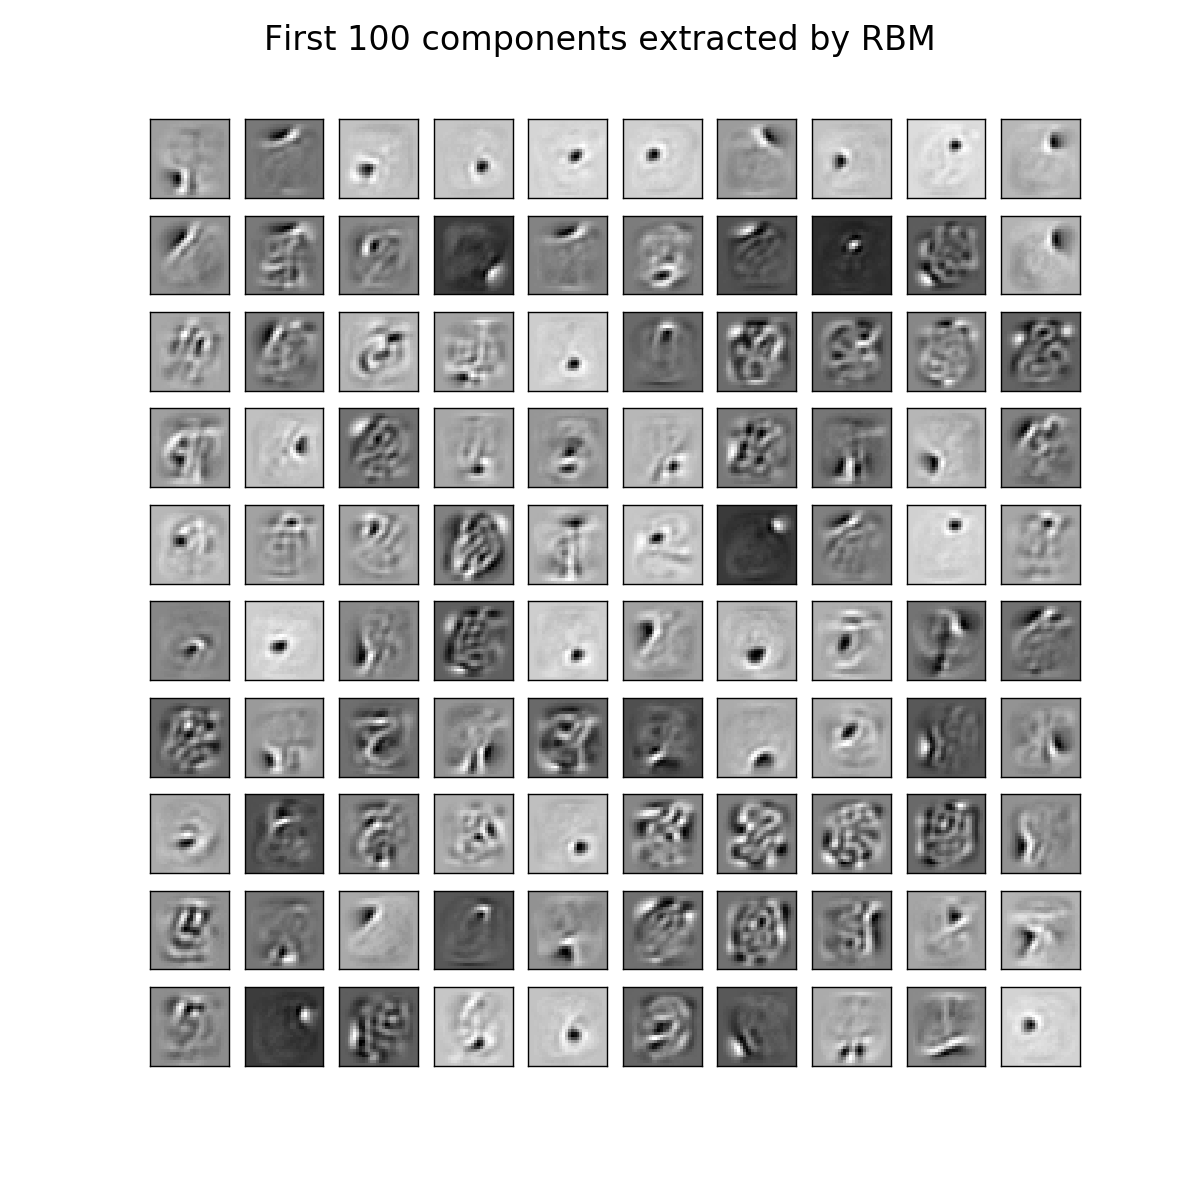
\includegraphics[width=.32\textwidth]{rbm-mnist/L1e-2.png}\quad
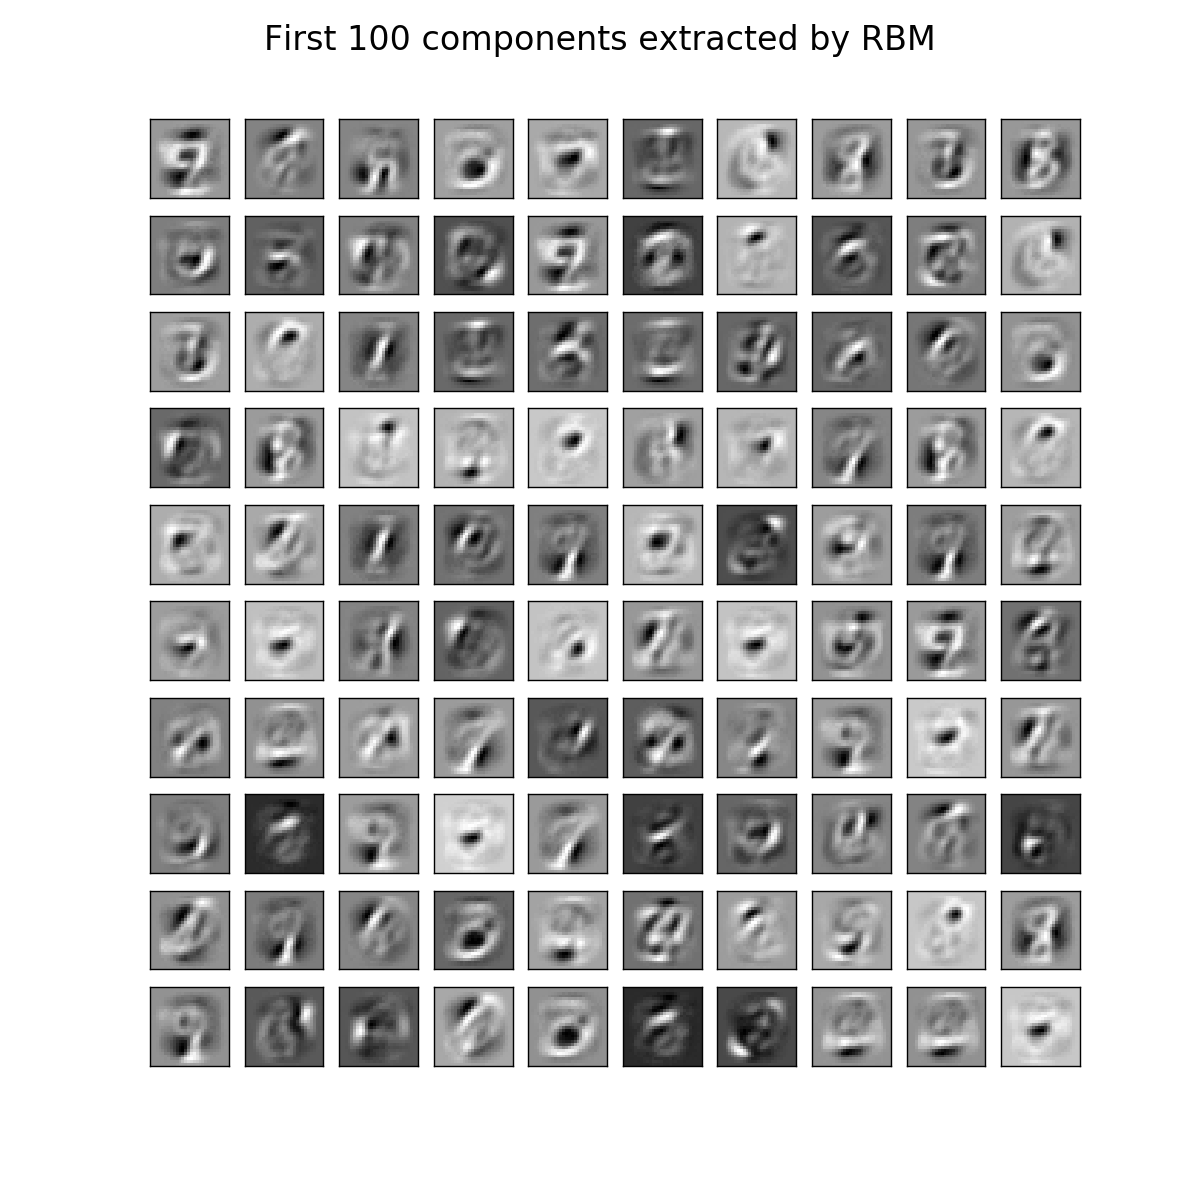
\includegraphics[width=.32\textwidth]{rbm-mnist/L1e-1.png}

\medskip

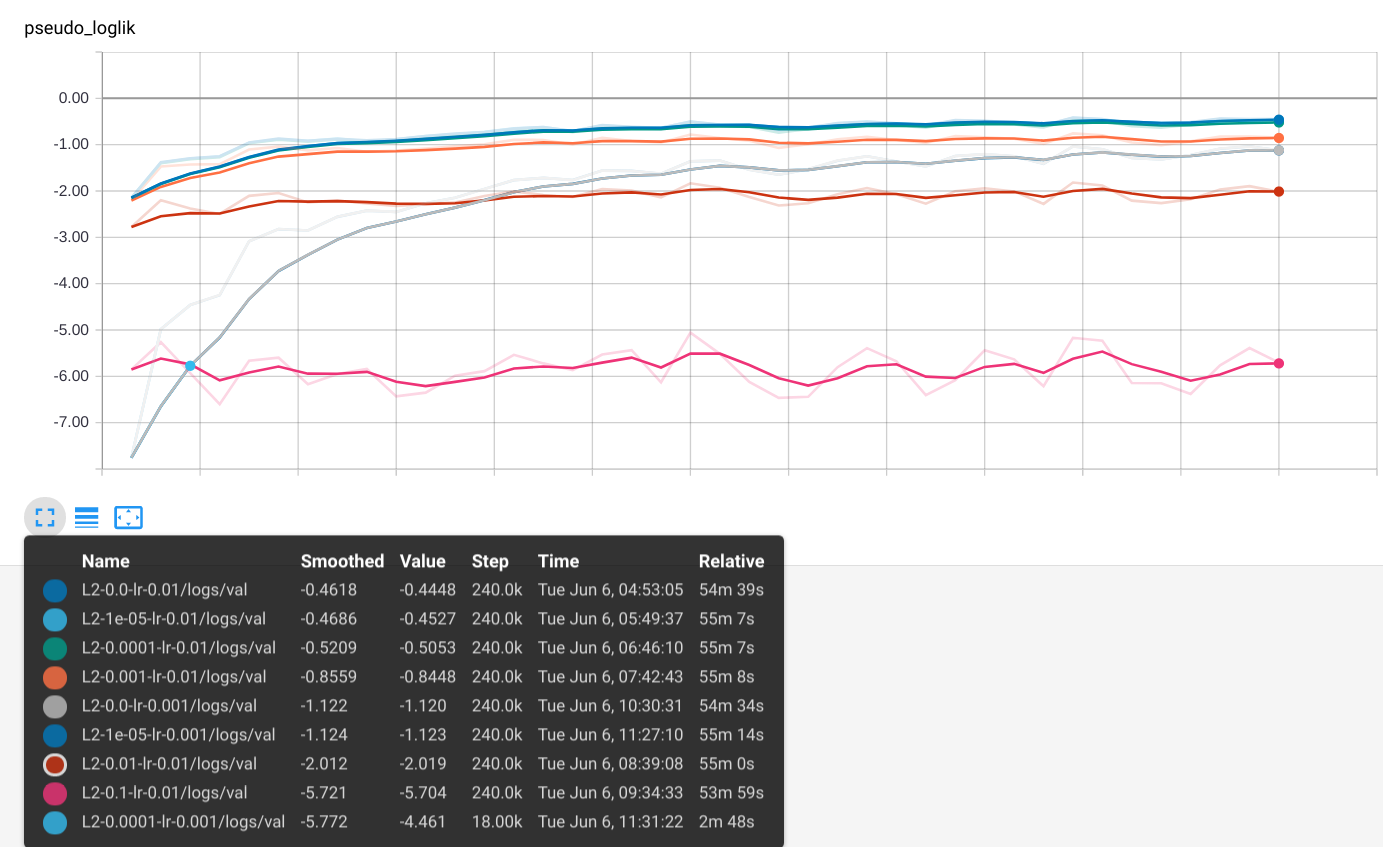
\includegraphics[width=.9\textwidth]{rbm-mnist/L2_pll.png}
\caption{Different amount of regularization. \emph{Left to right, top to bottom}, $\lambda=10^{-5}\ldots10^{-1}$. \emph{Bottom}: PLL of RBM as $\lambda$ varies.}
\end{mdframed}
\end{figure*}

\clearpage

\begin{figure}[h]
\begin{mdframed}
\centering
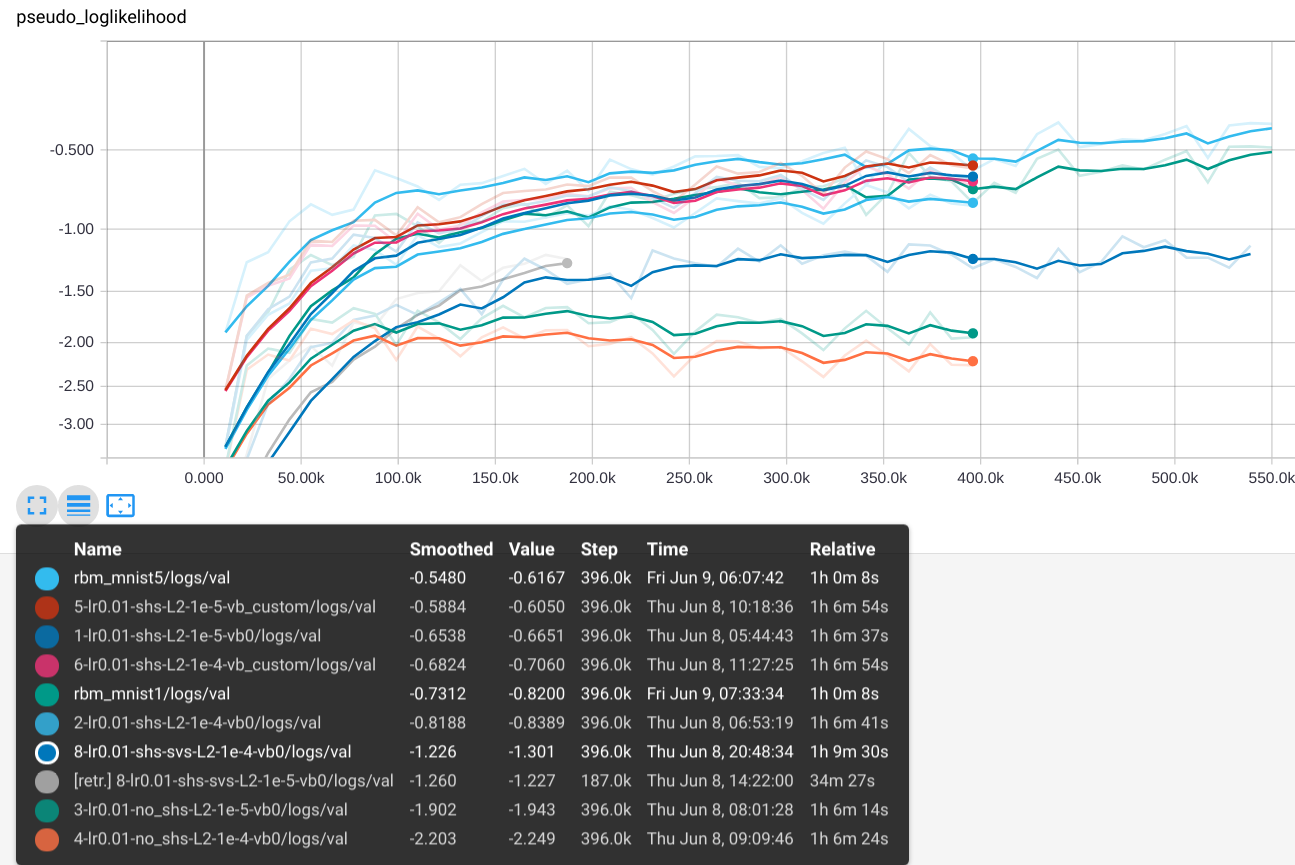
\includegraphics[width=4.6in]{rbm-mnist/rbm_practical_full.png}
\\[1em]
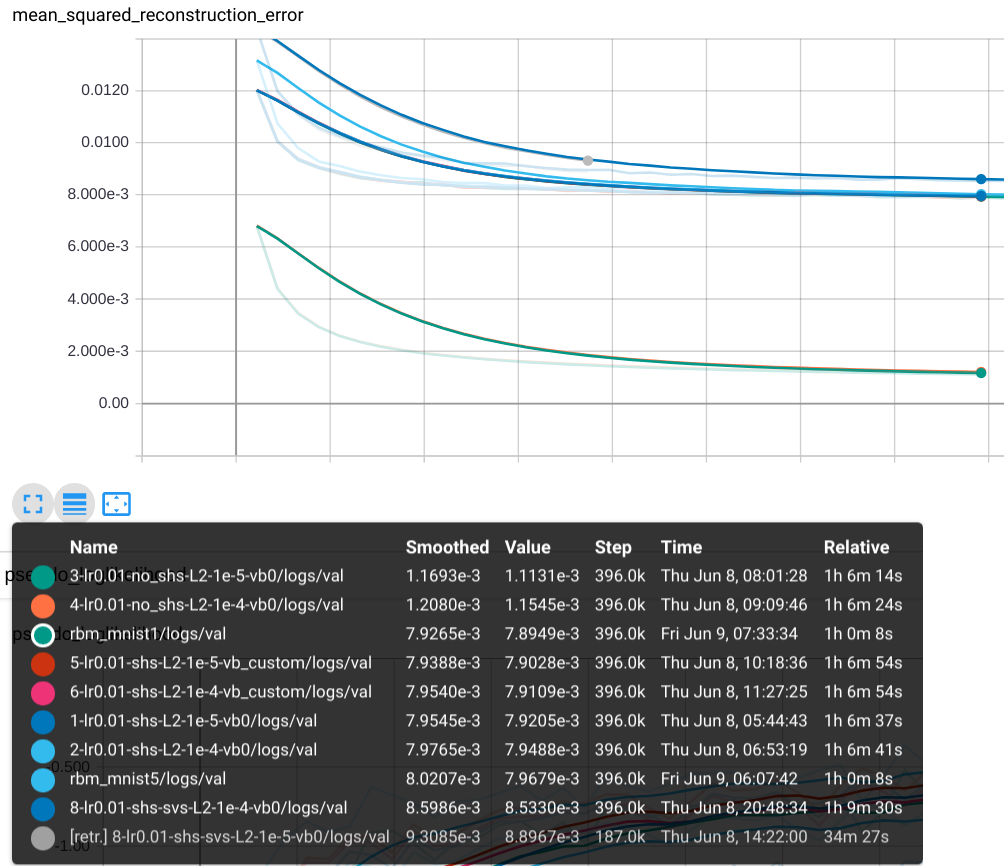
\includegraphics[width=4.6in]{rbm-mnist/recon_full.png}
\caption{PLL (top) and Reconstruction error (bottom) of RBMs trained using various approaches on full MNIST dataset. It is an example when you shouldn't trust reconstruction error: models with lowest values of this quantity have very poor PLL.}
\end{mdframed}
\end{figure}

\clearpage

\begin{figure}[h]
\begin{mdframed}
\centering
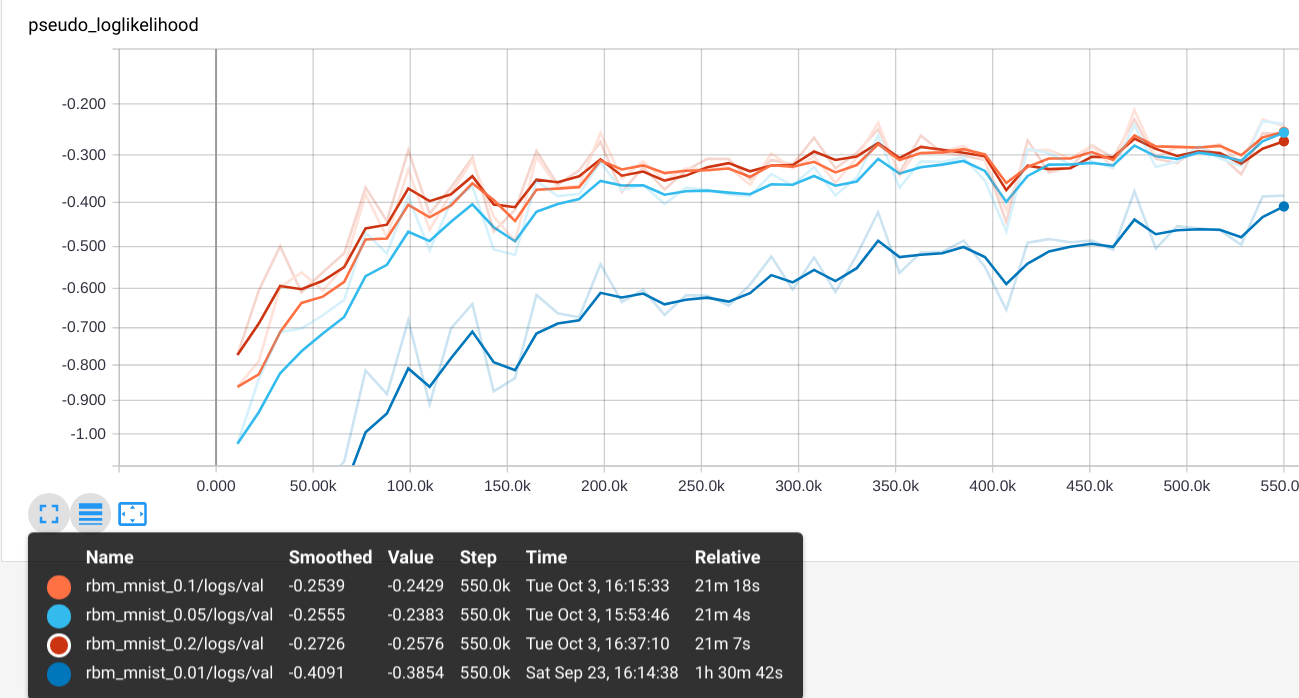
\includegraphics[width=5.6in]{rbm-mnist/pll_lr.png}
\\[2em]
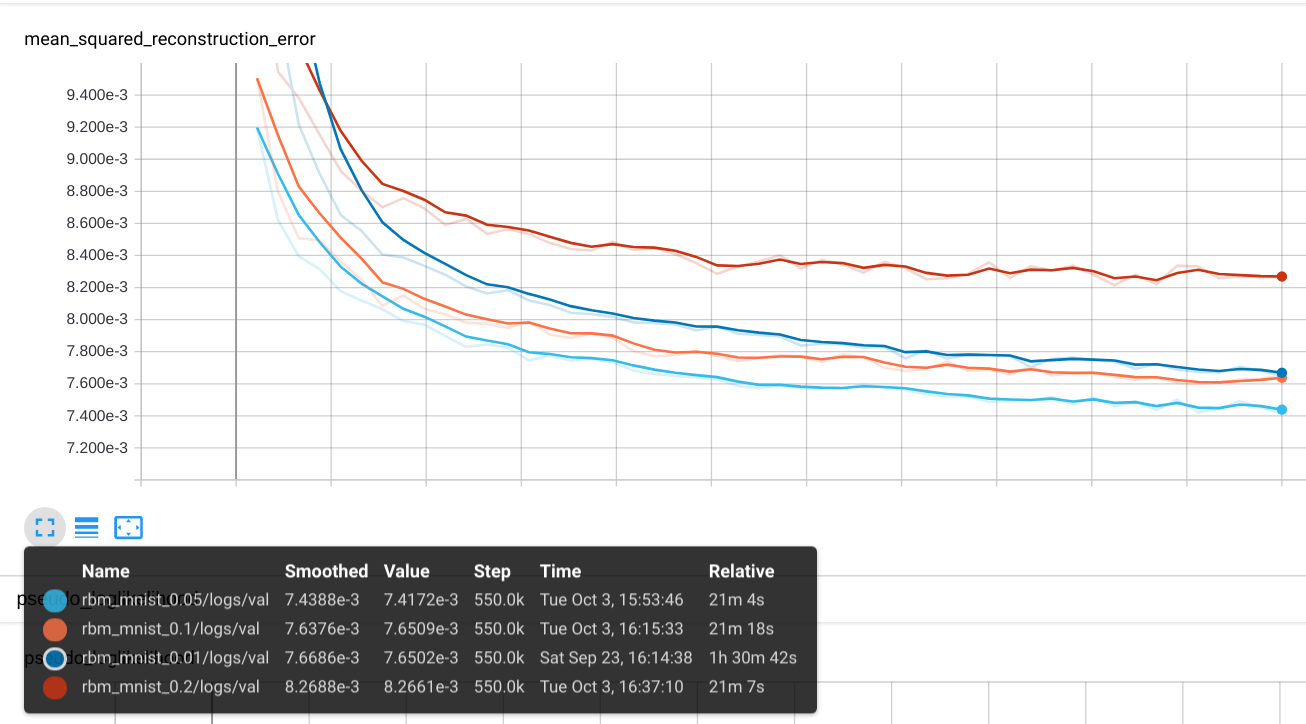
\includegraphics[width=5.6in]{rbm-mnist/msre_lr.png}
\caption{PLL and reconstruction error as learning rate varies (full MNIST).}
\end{mdframed}
\end{figure}

\clearpage

\begin{figure}[h]
\begin{mdframed}
\centering
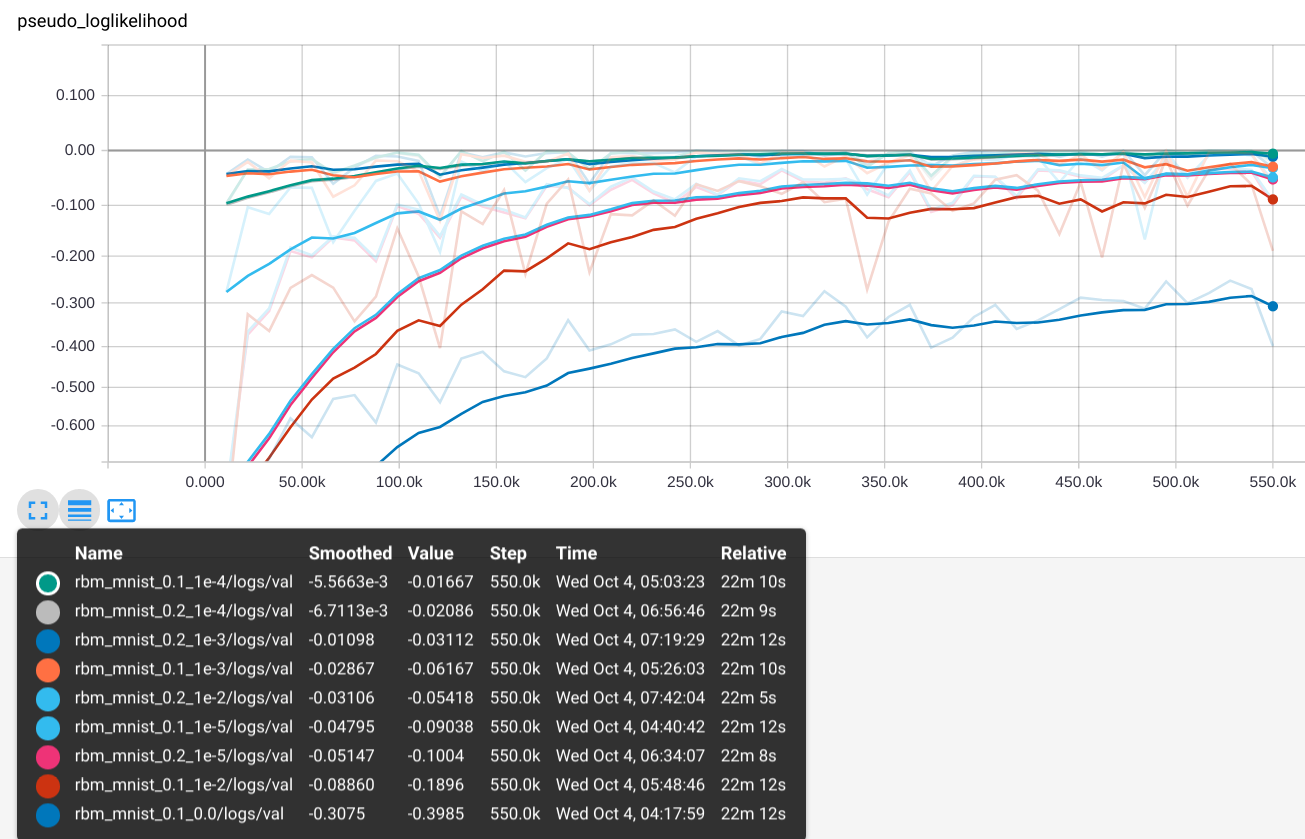
\includegraphics[width=5.6in]{rbm-mnist/st_pll.png}
\\[2em]
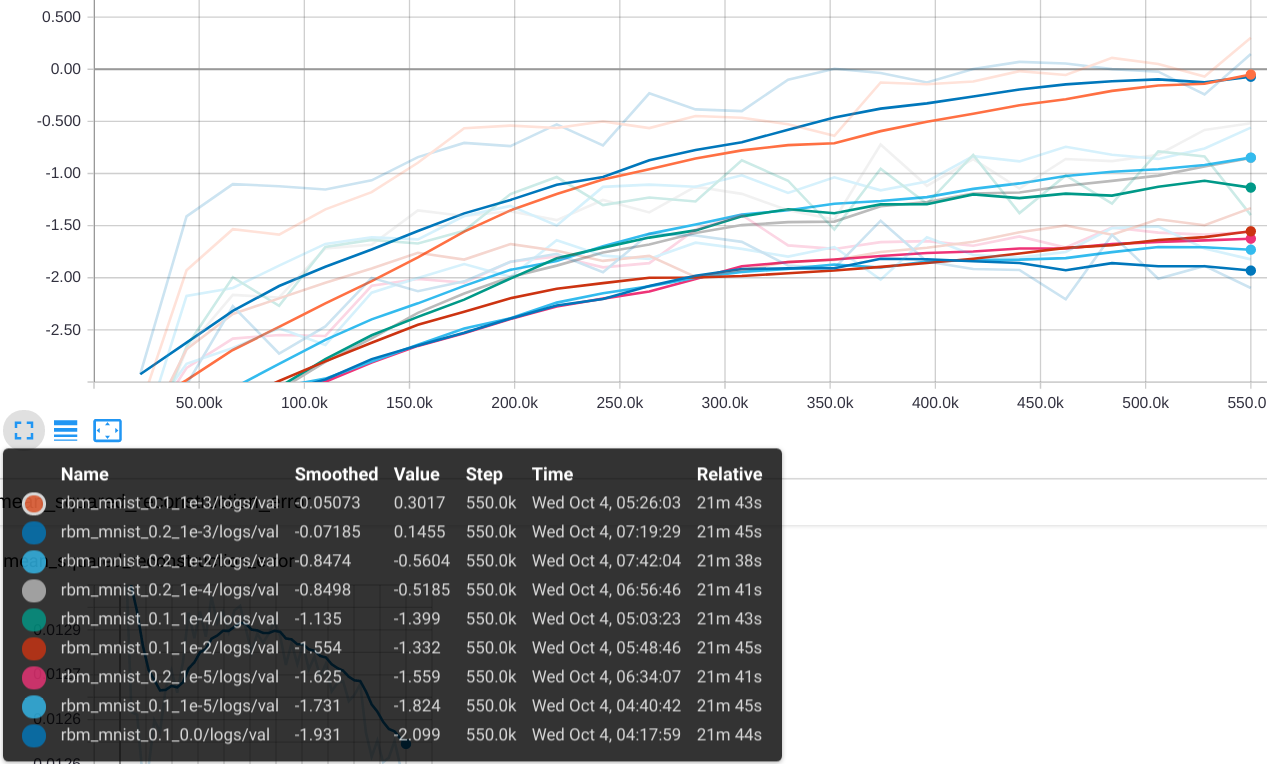
\includegraphics[width=5.6in]{rbm-mnist/st_feg.png}
\caption{PLL and free energy gap for sparsity target $t\in\{0,1\}$ and sparsity cost $\lambda \in \{0, 10^{-5\;\tb{:}\;-2}\}$ are used (full MNIST).}
\end{mdframed}
\end{figure}

\clearpage

\begin{figure}[h]
\begin{mdframed}
\centering
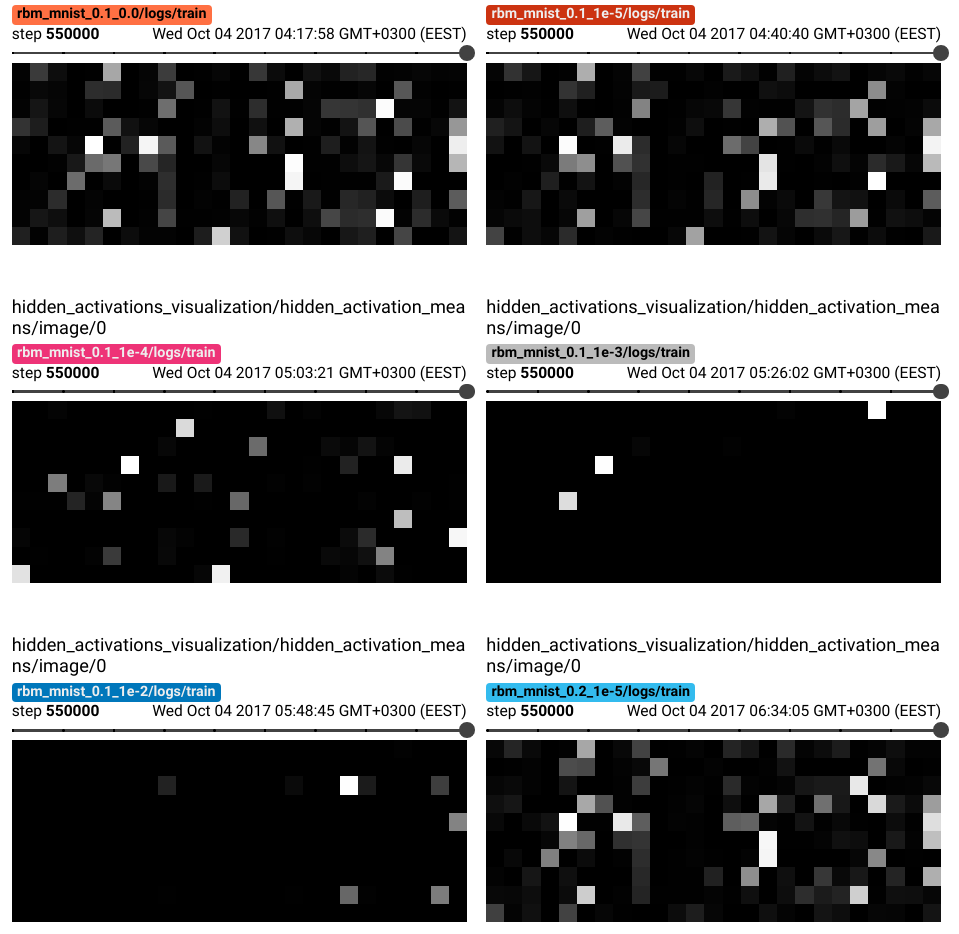
\includegraphics[width=4.8in]{rbm-mnist/st_hidden_activations.png}
\\[4em]
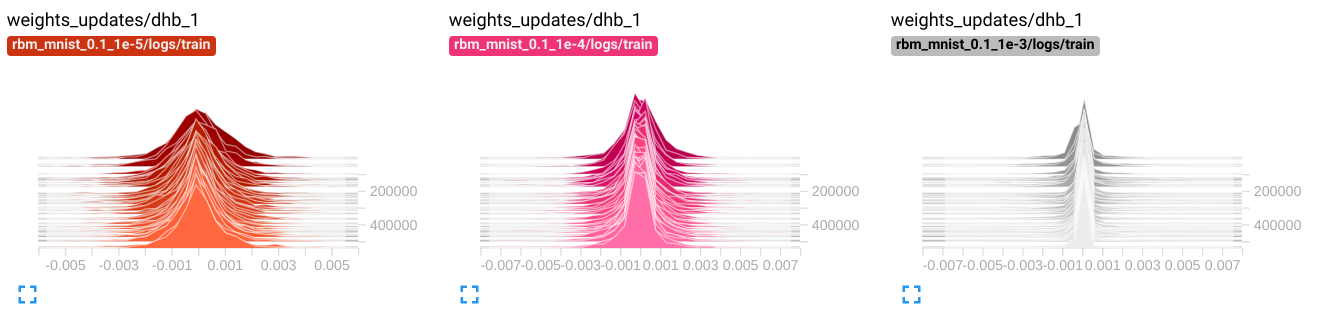
\includegraphics[width=5.6in]{rbm-mnist/st_hb_updates.png}
\caption{Hidden activations and hidden bias updates distributions from previous experiment. We clearly see that for larger $\lambda$ hidden activities become more and more sparse and distribtion becomes more and more peaky (same for weight updates).}
\end{mdframed}
\end{figure}

\clearpage

\begin{figure*}[t!]
\begin{mdframed}
\centering
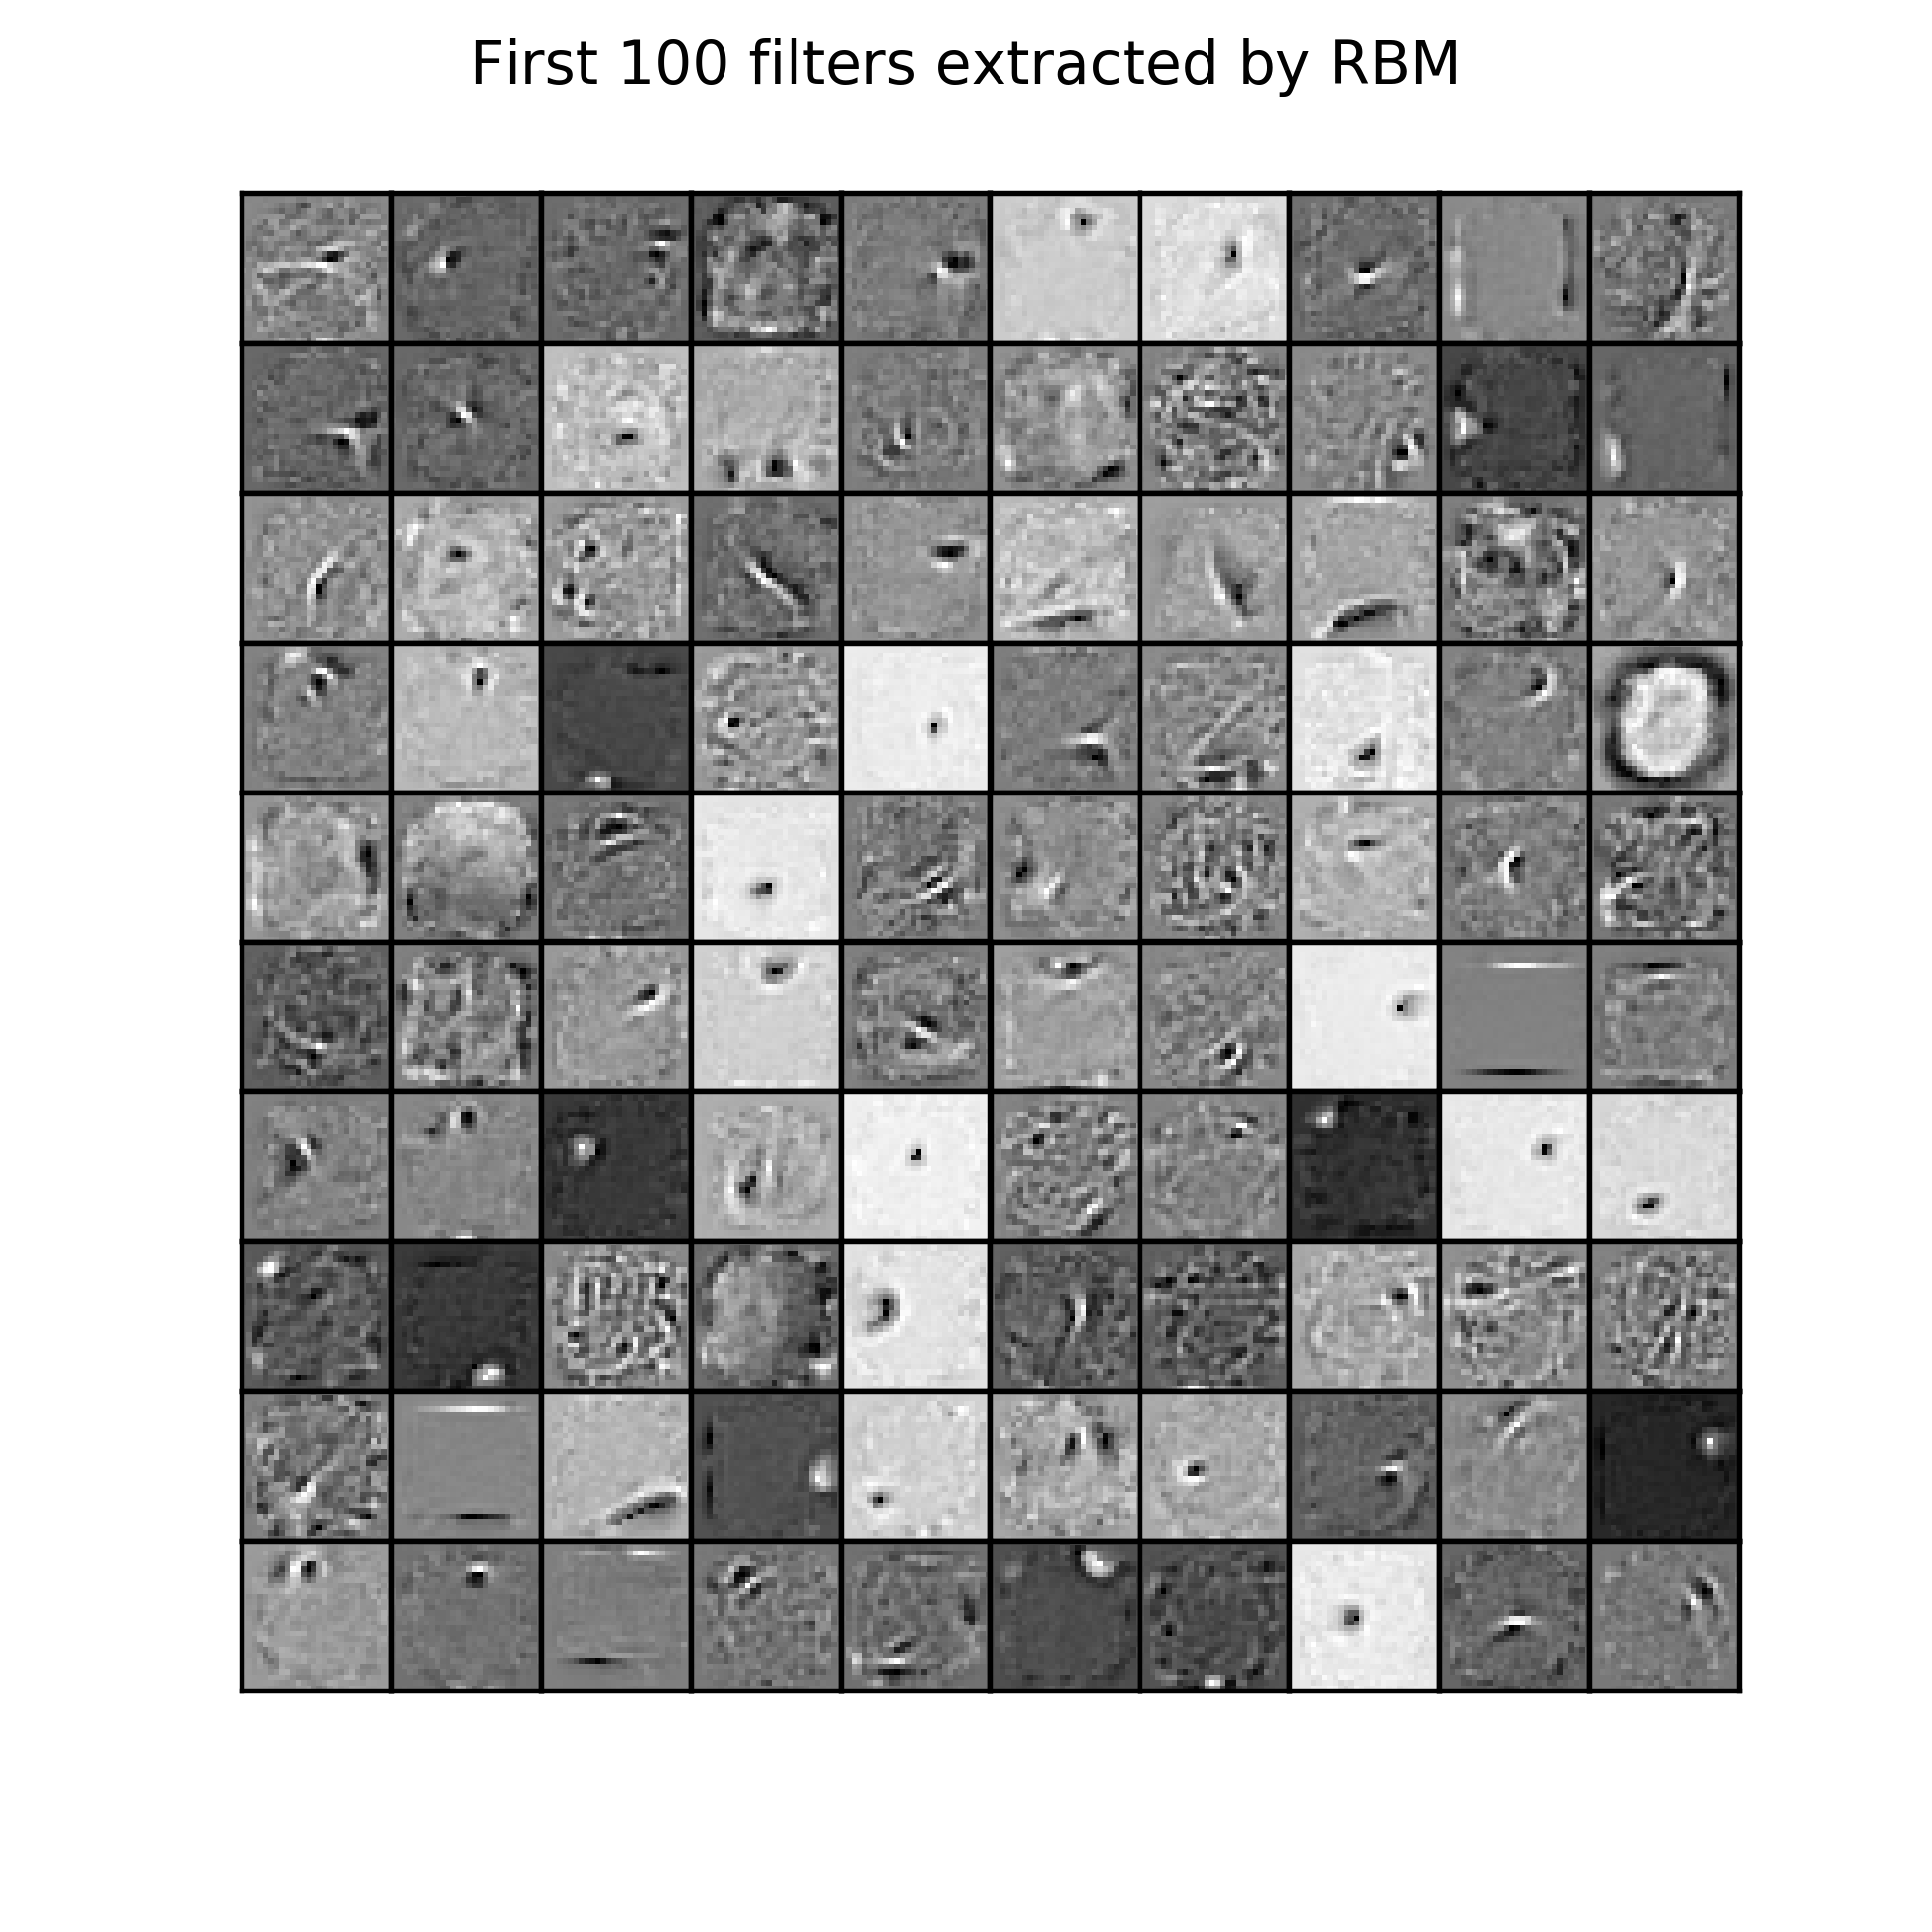
\includegraphics[width=.31\textwidth]{rbm-mnist/st_rbm_mnist_0.png}\quad
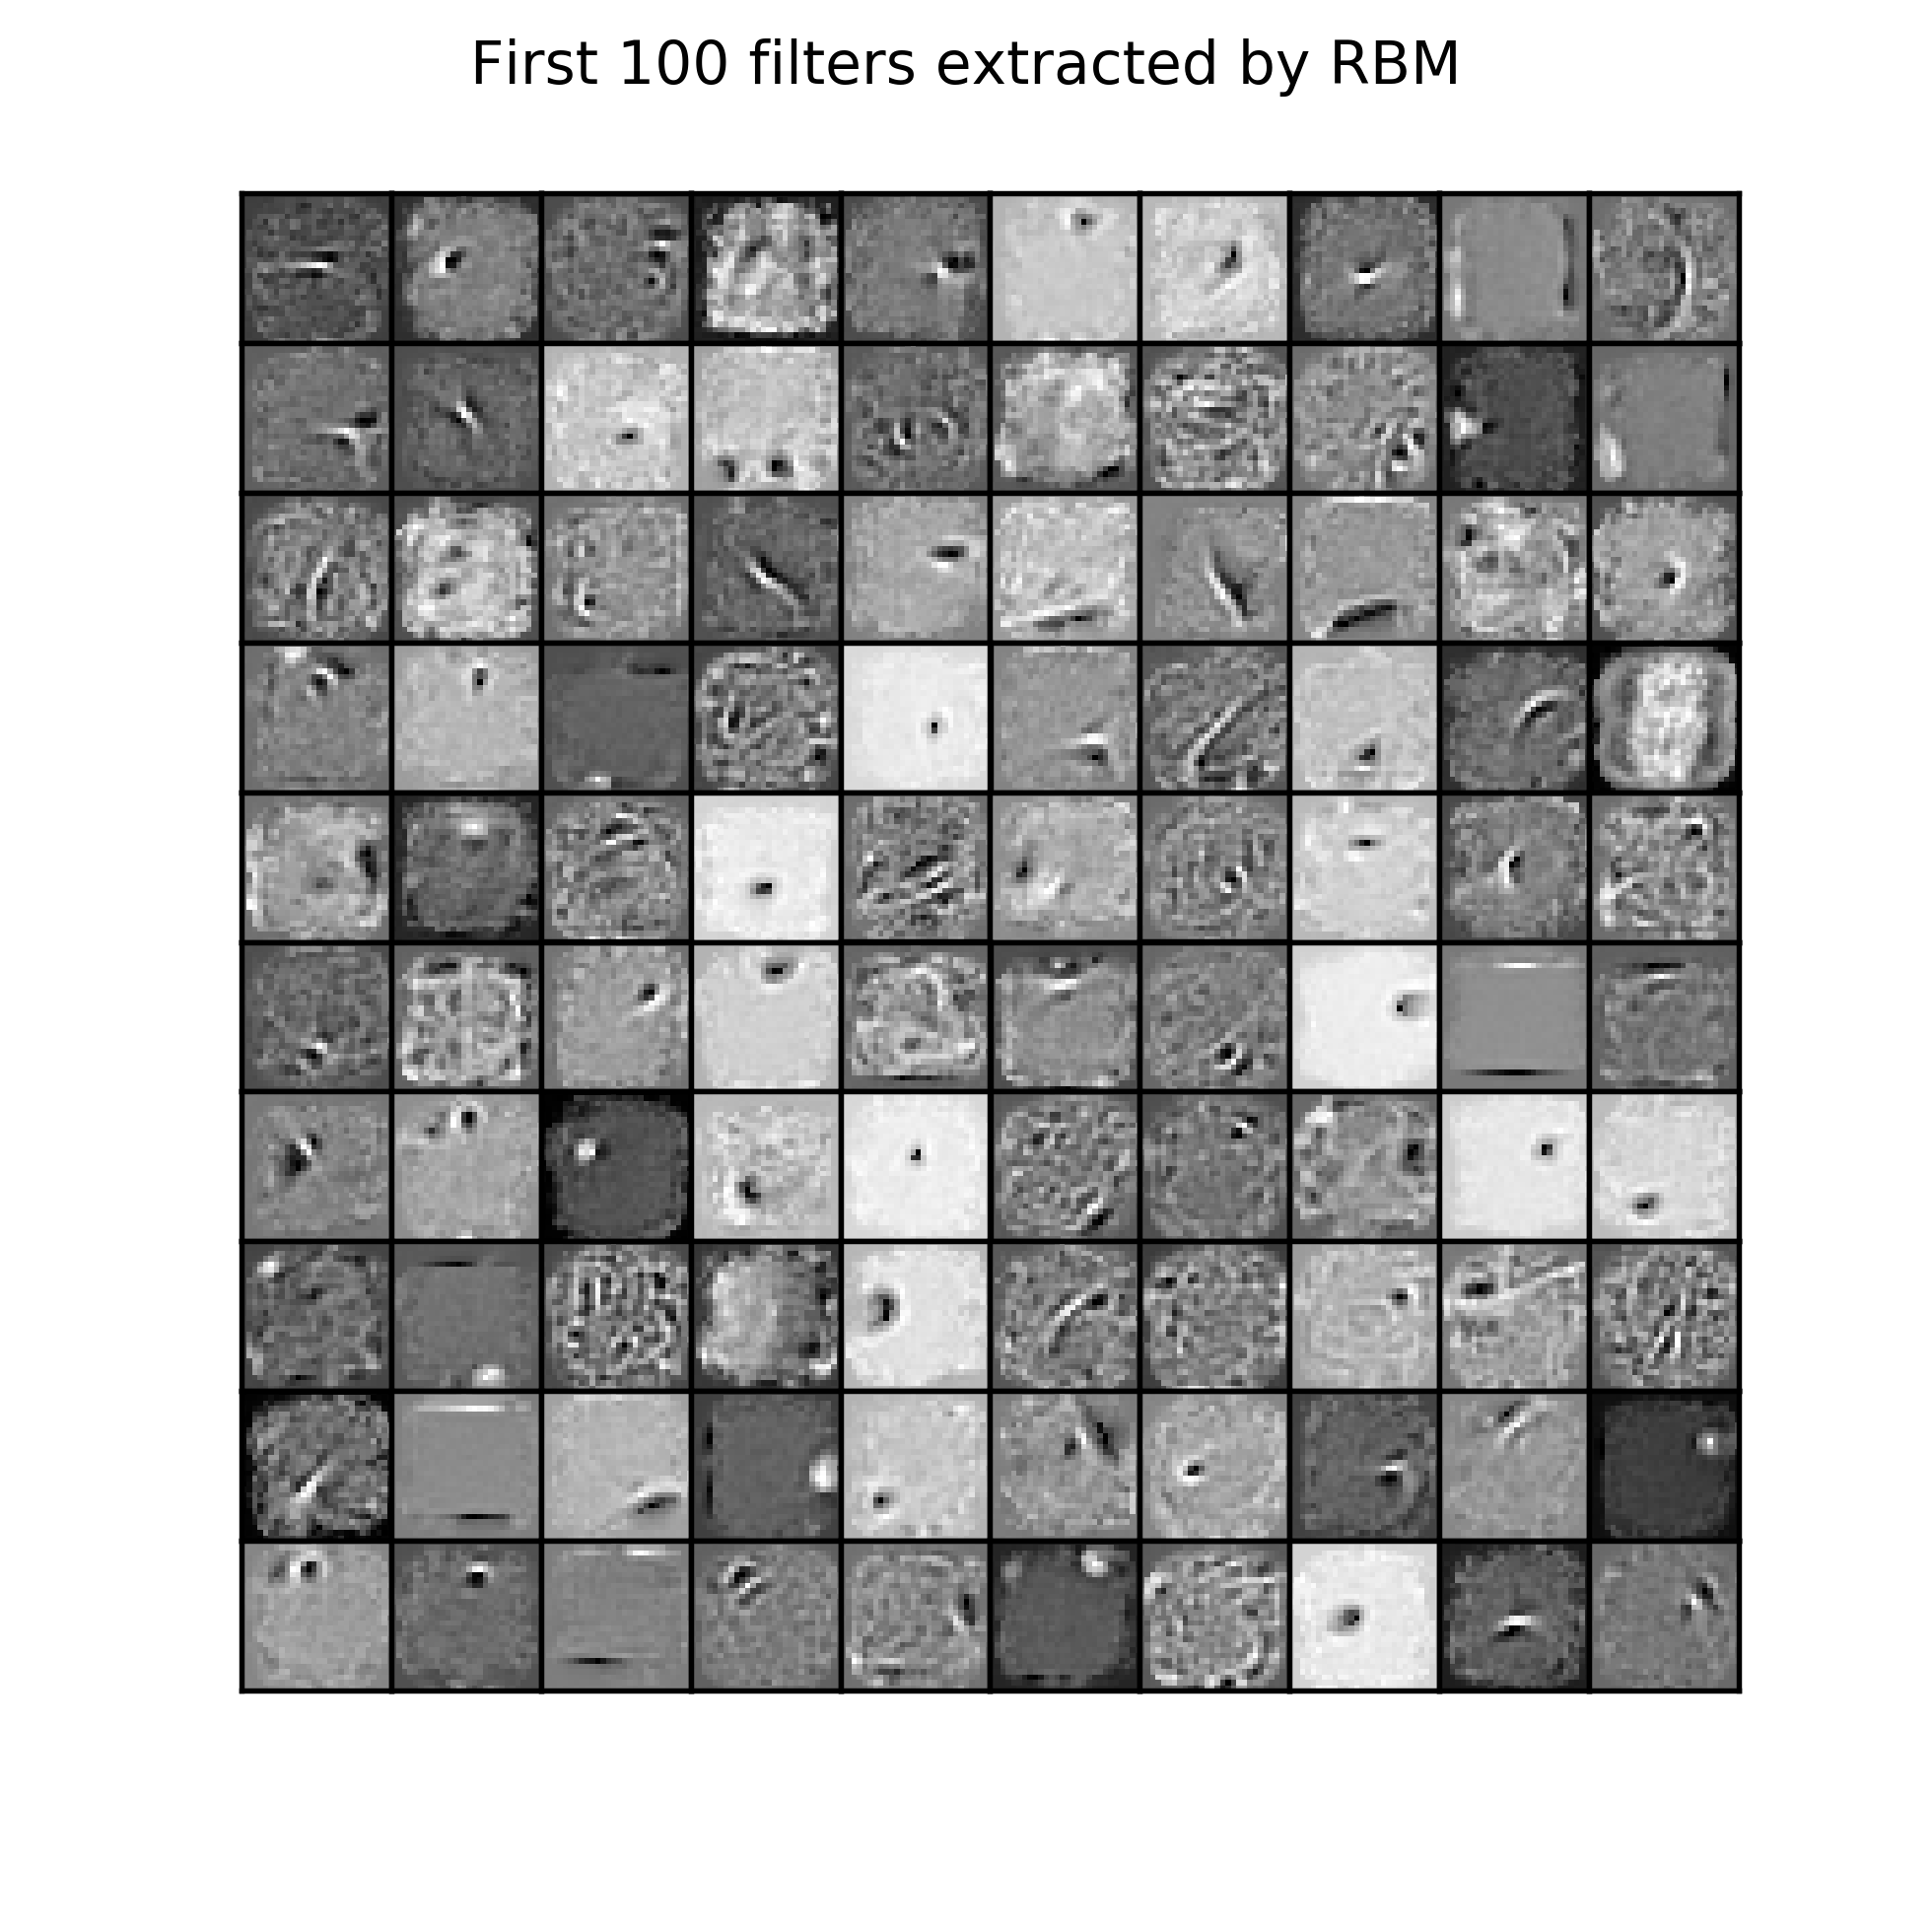
\includegraphics[width=.31\textwidth]{rbm-mnist/st_rbm_mnist_1e-5.png}\quad
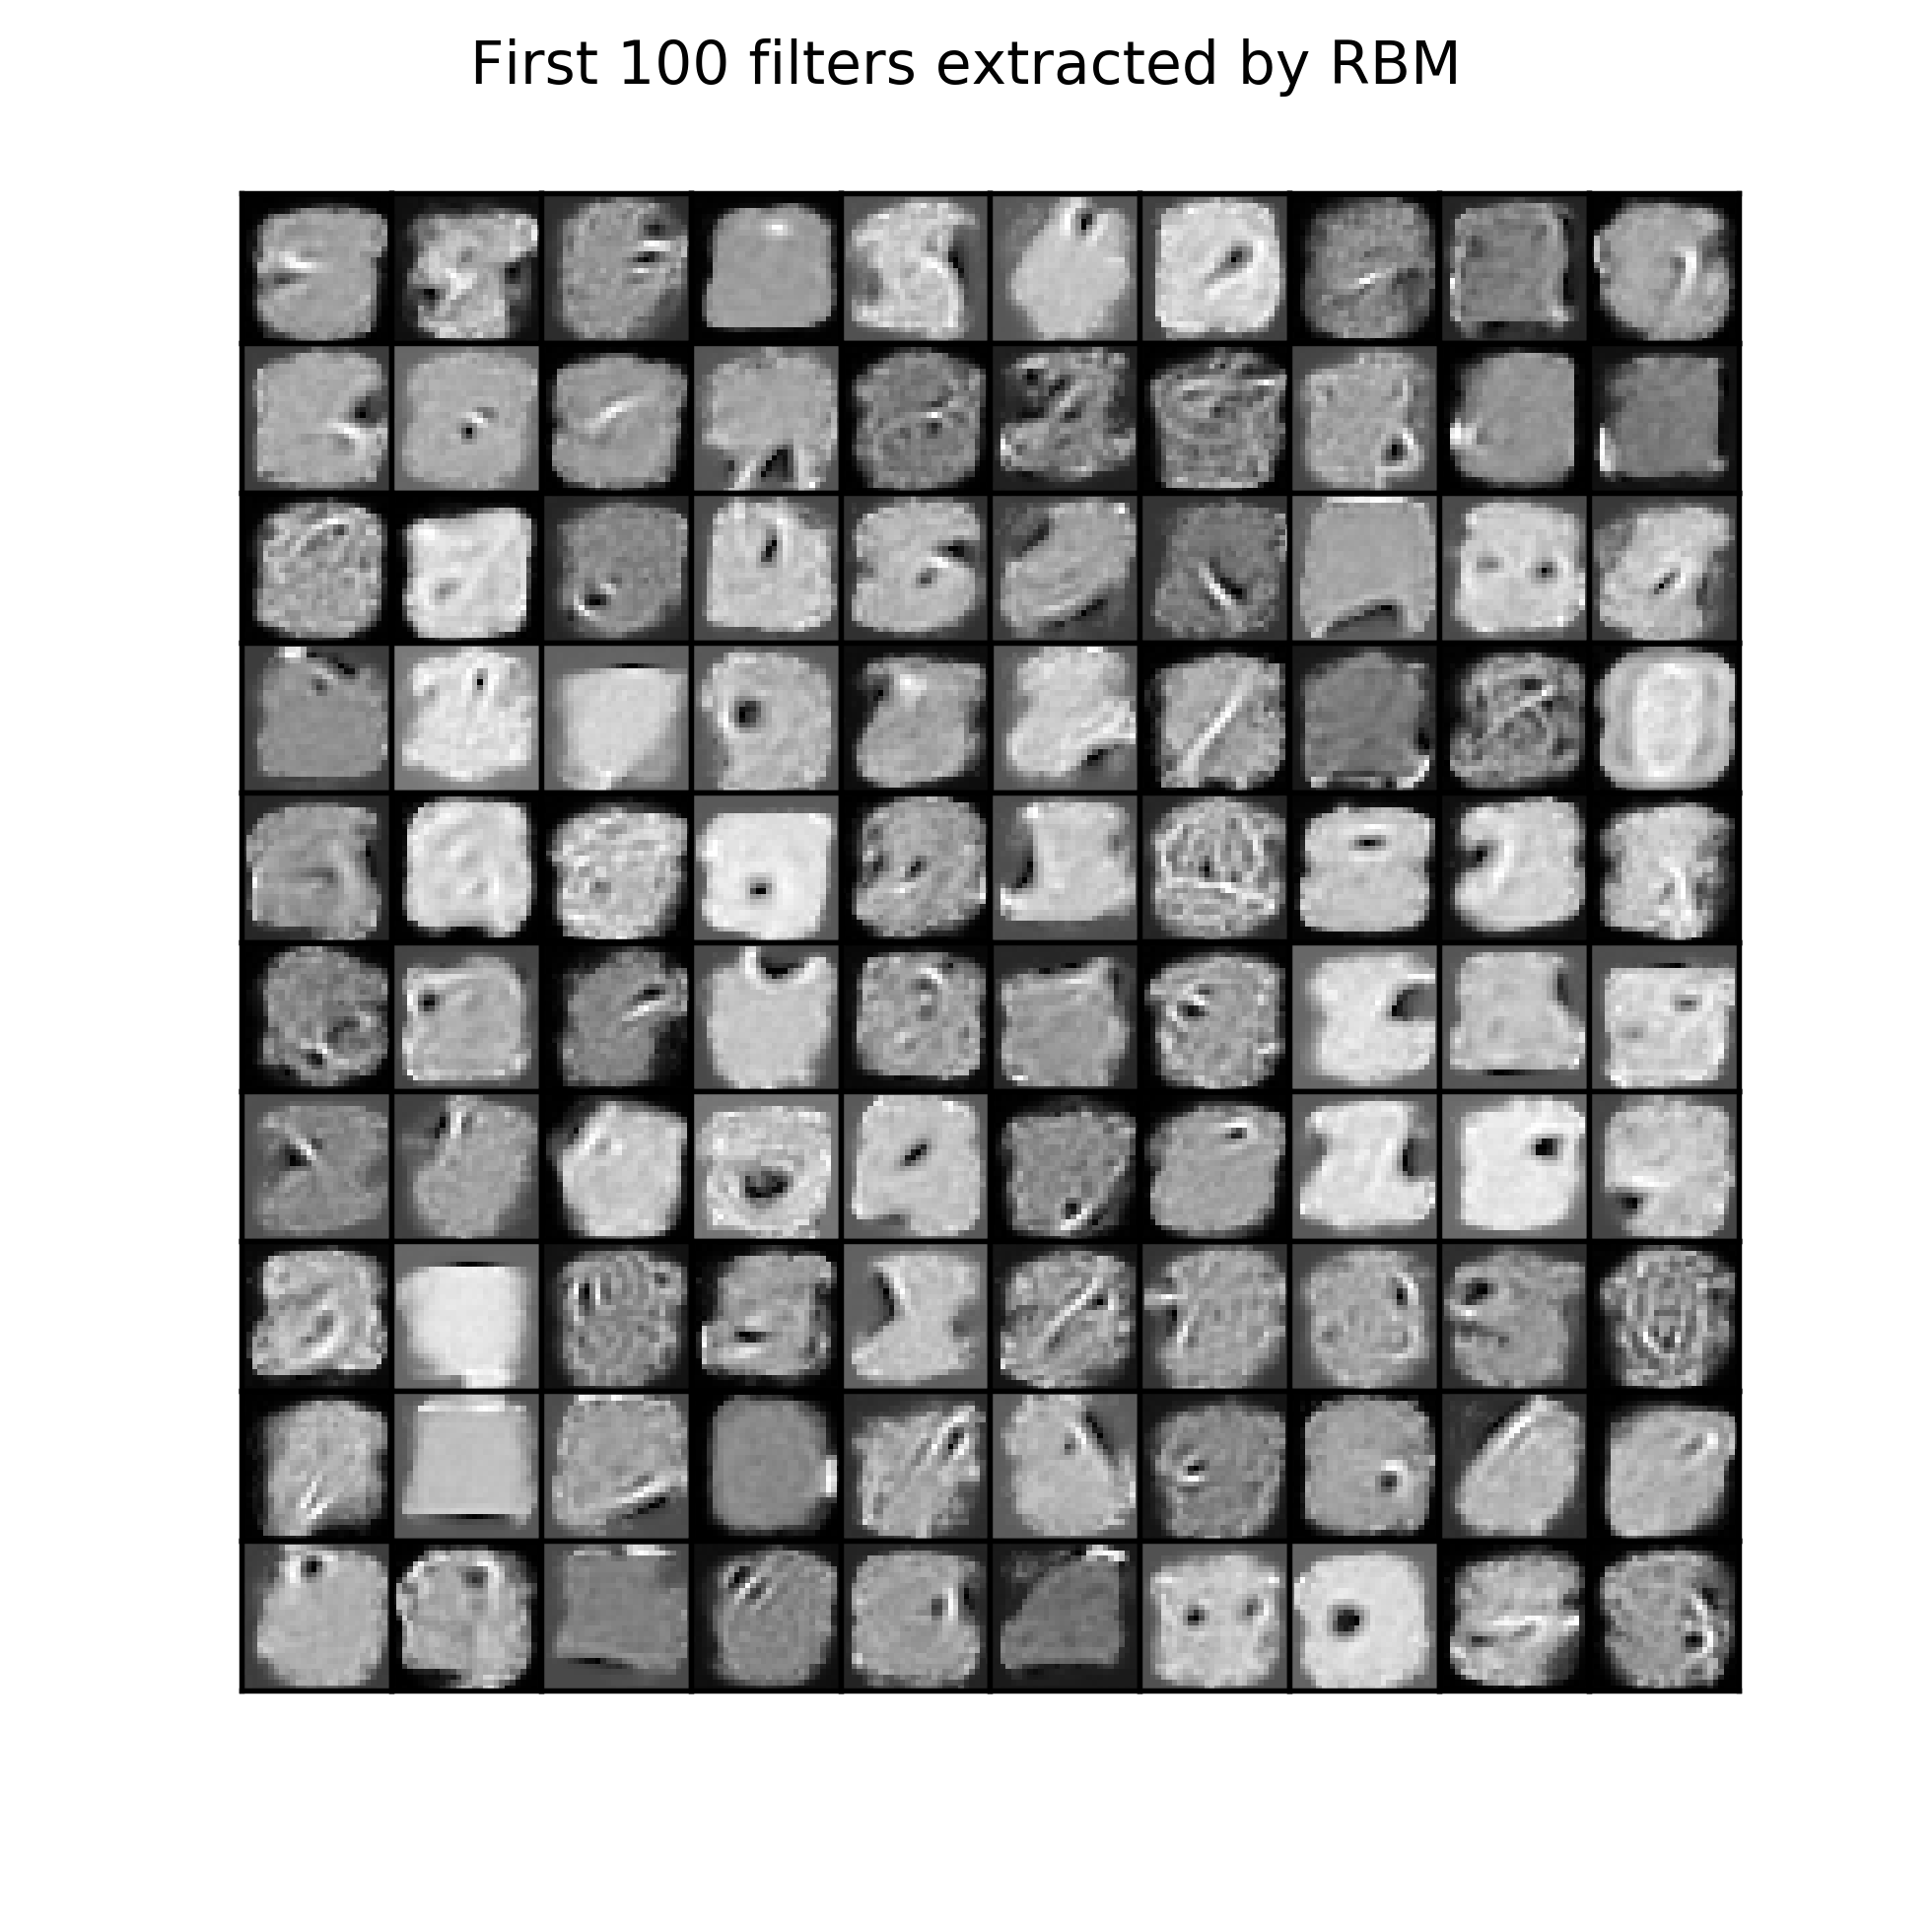
\includegraphics[width=.31\textwidth]{rbm-mnist/st_rbm_mnist_1e-4.png}

\medskip

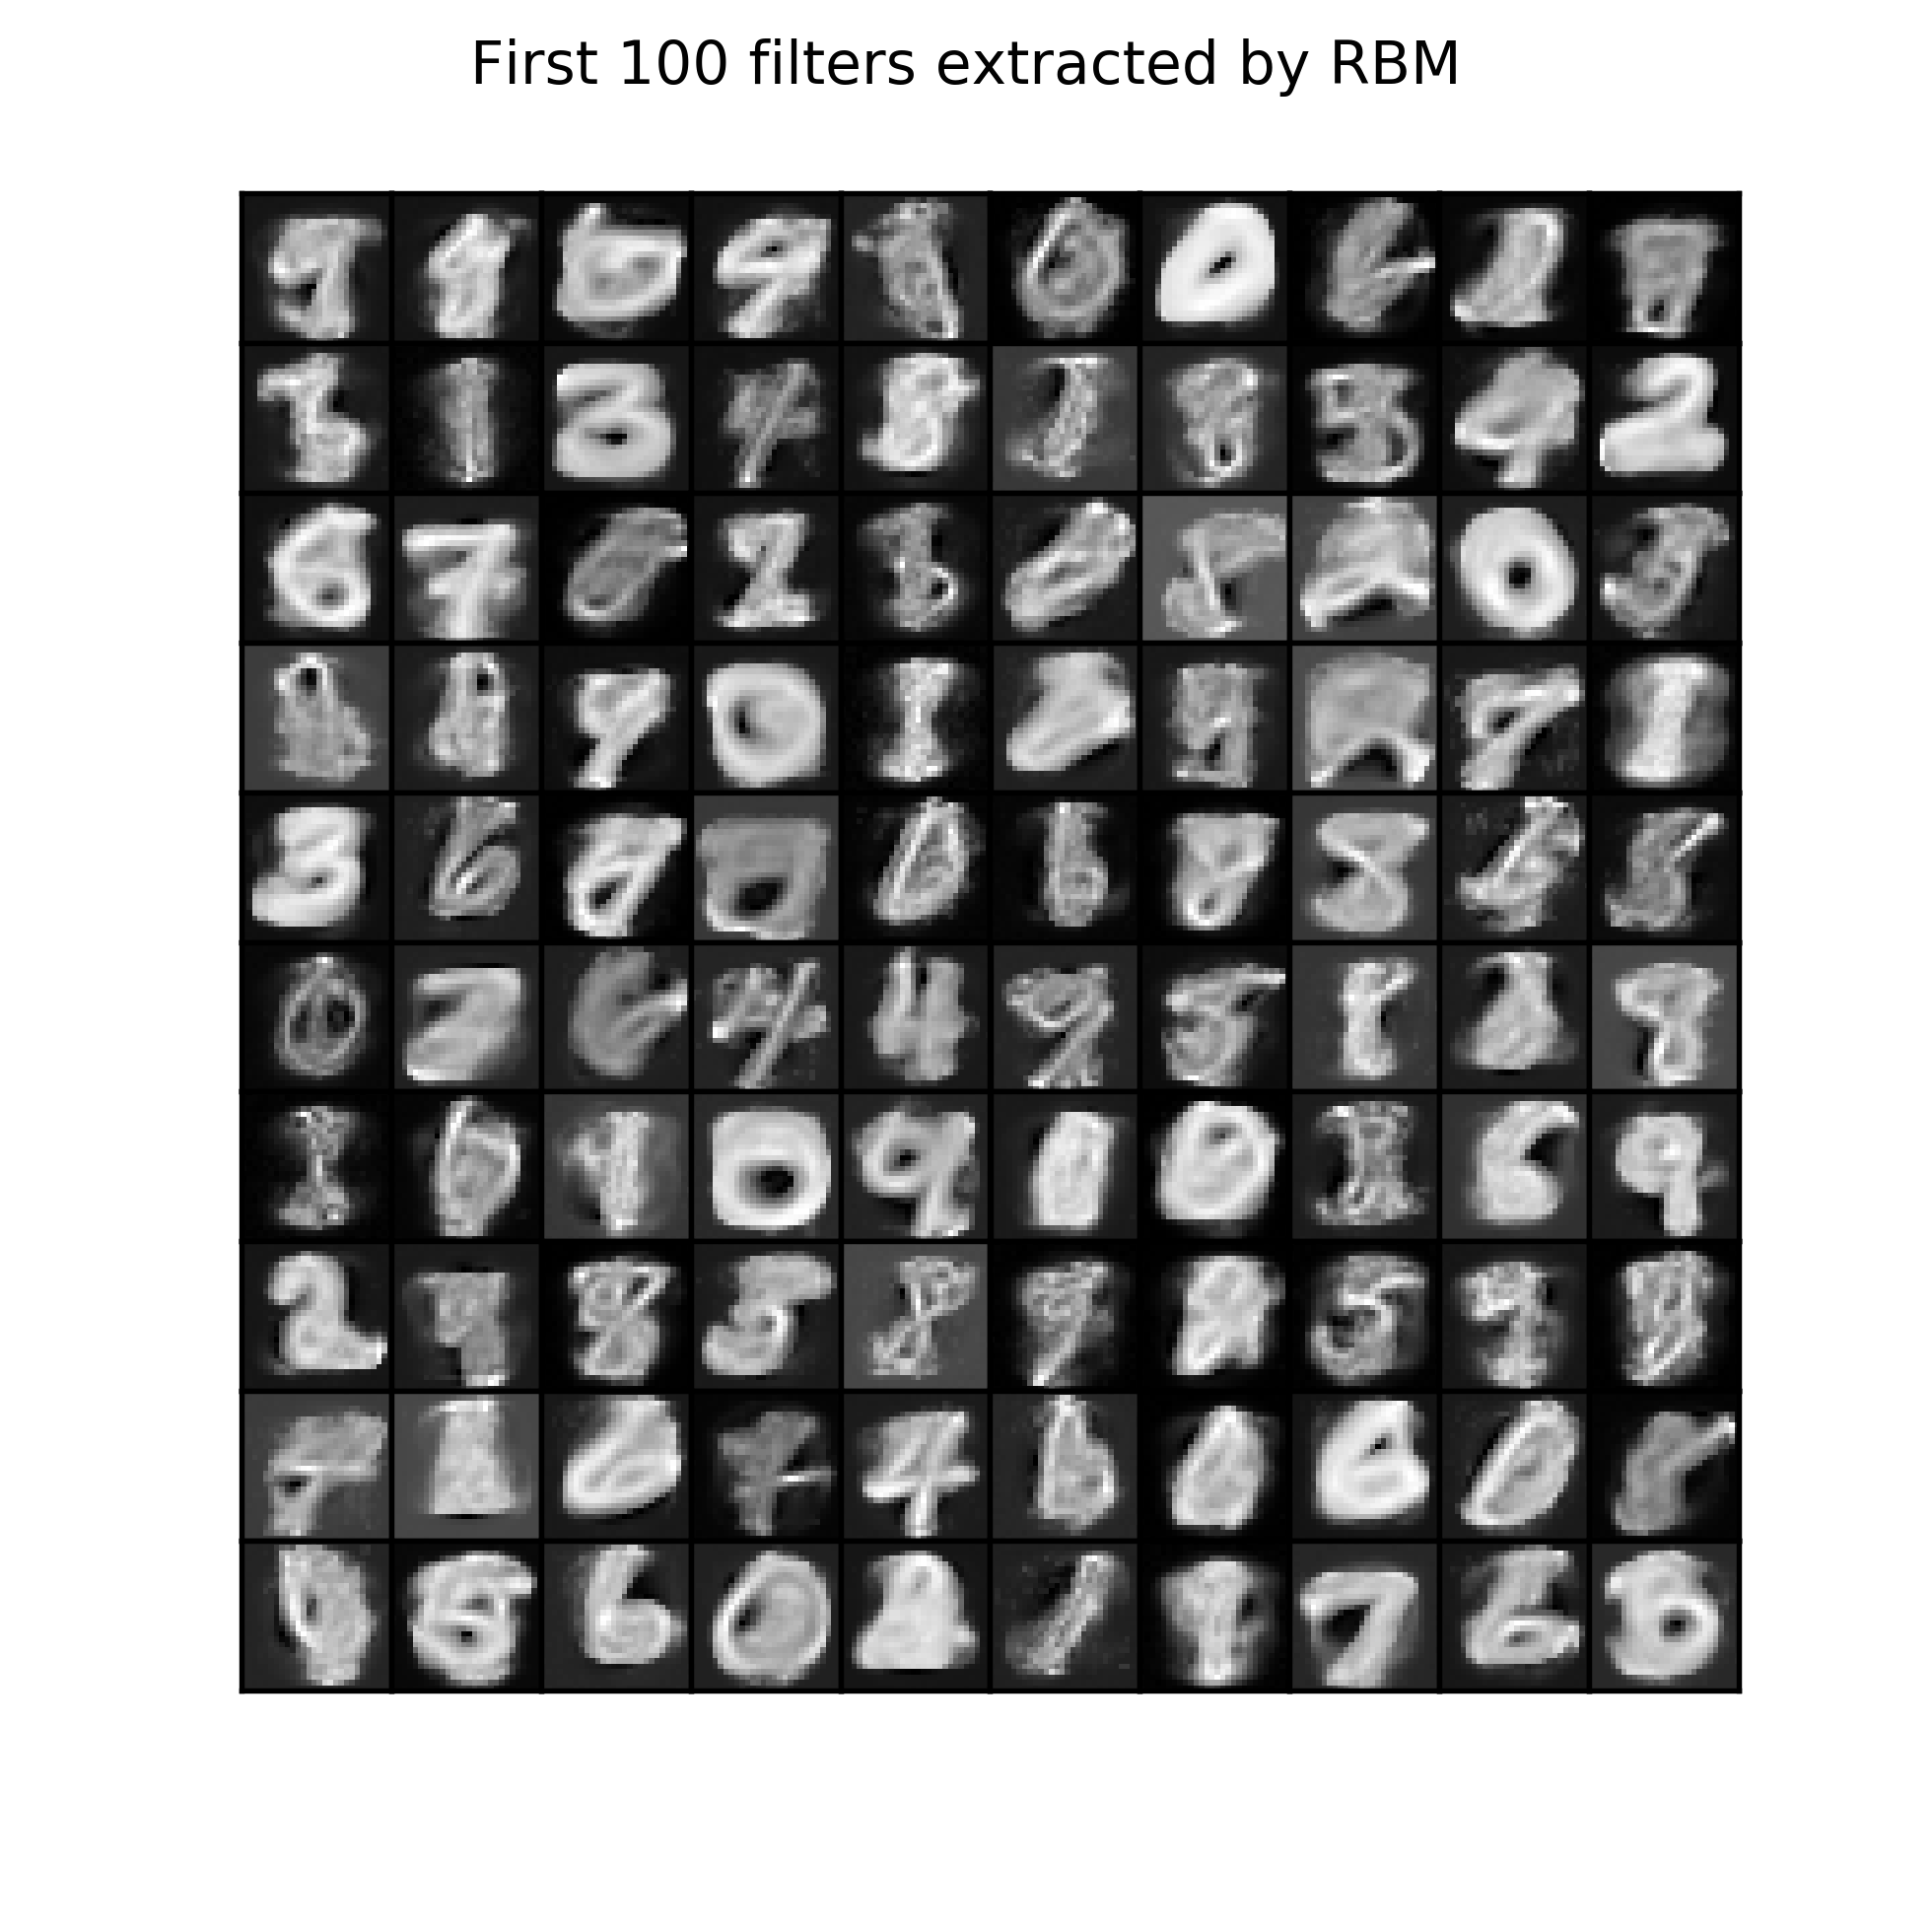
\includegraphics[width=.32\textwidth]{rbm-mnist/st_rbm_mnist_1e-3.png}\quad
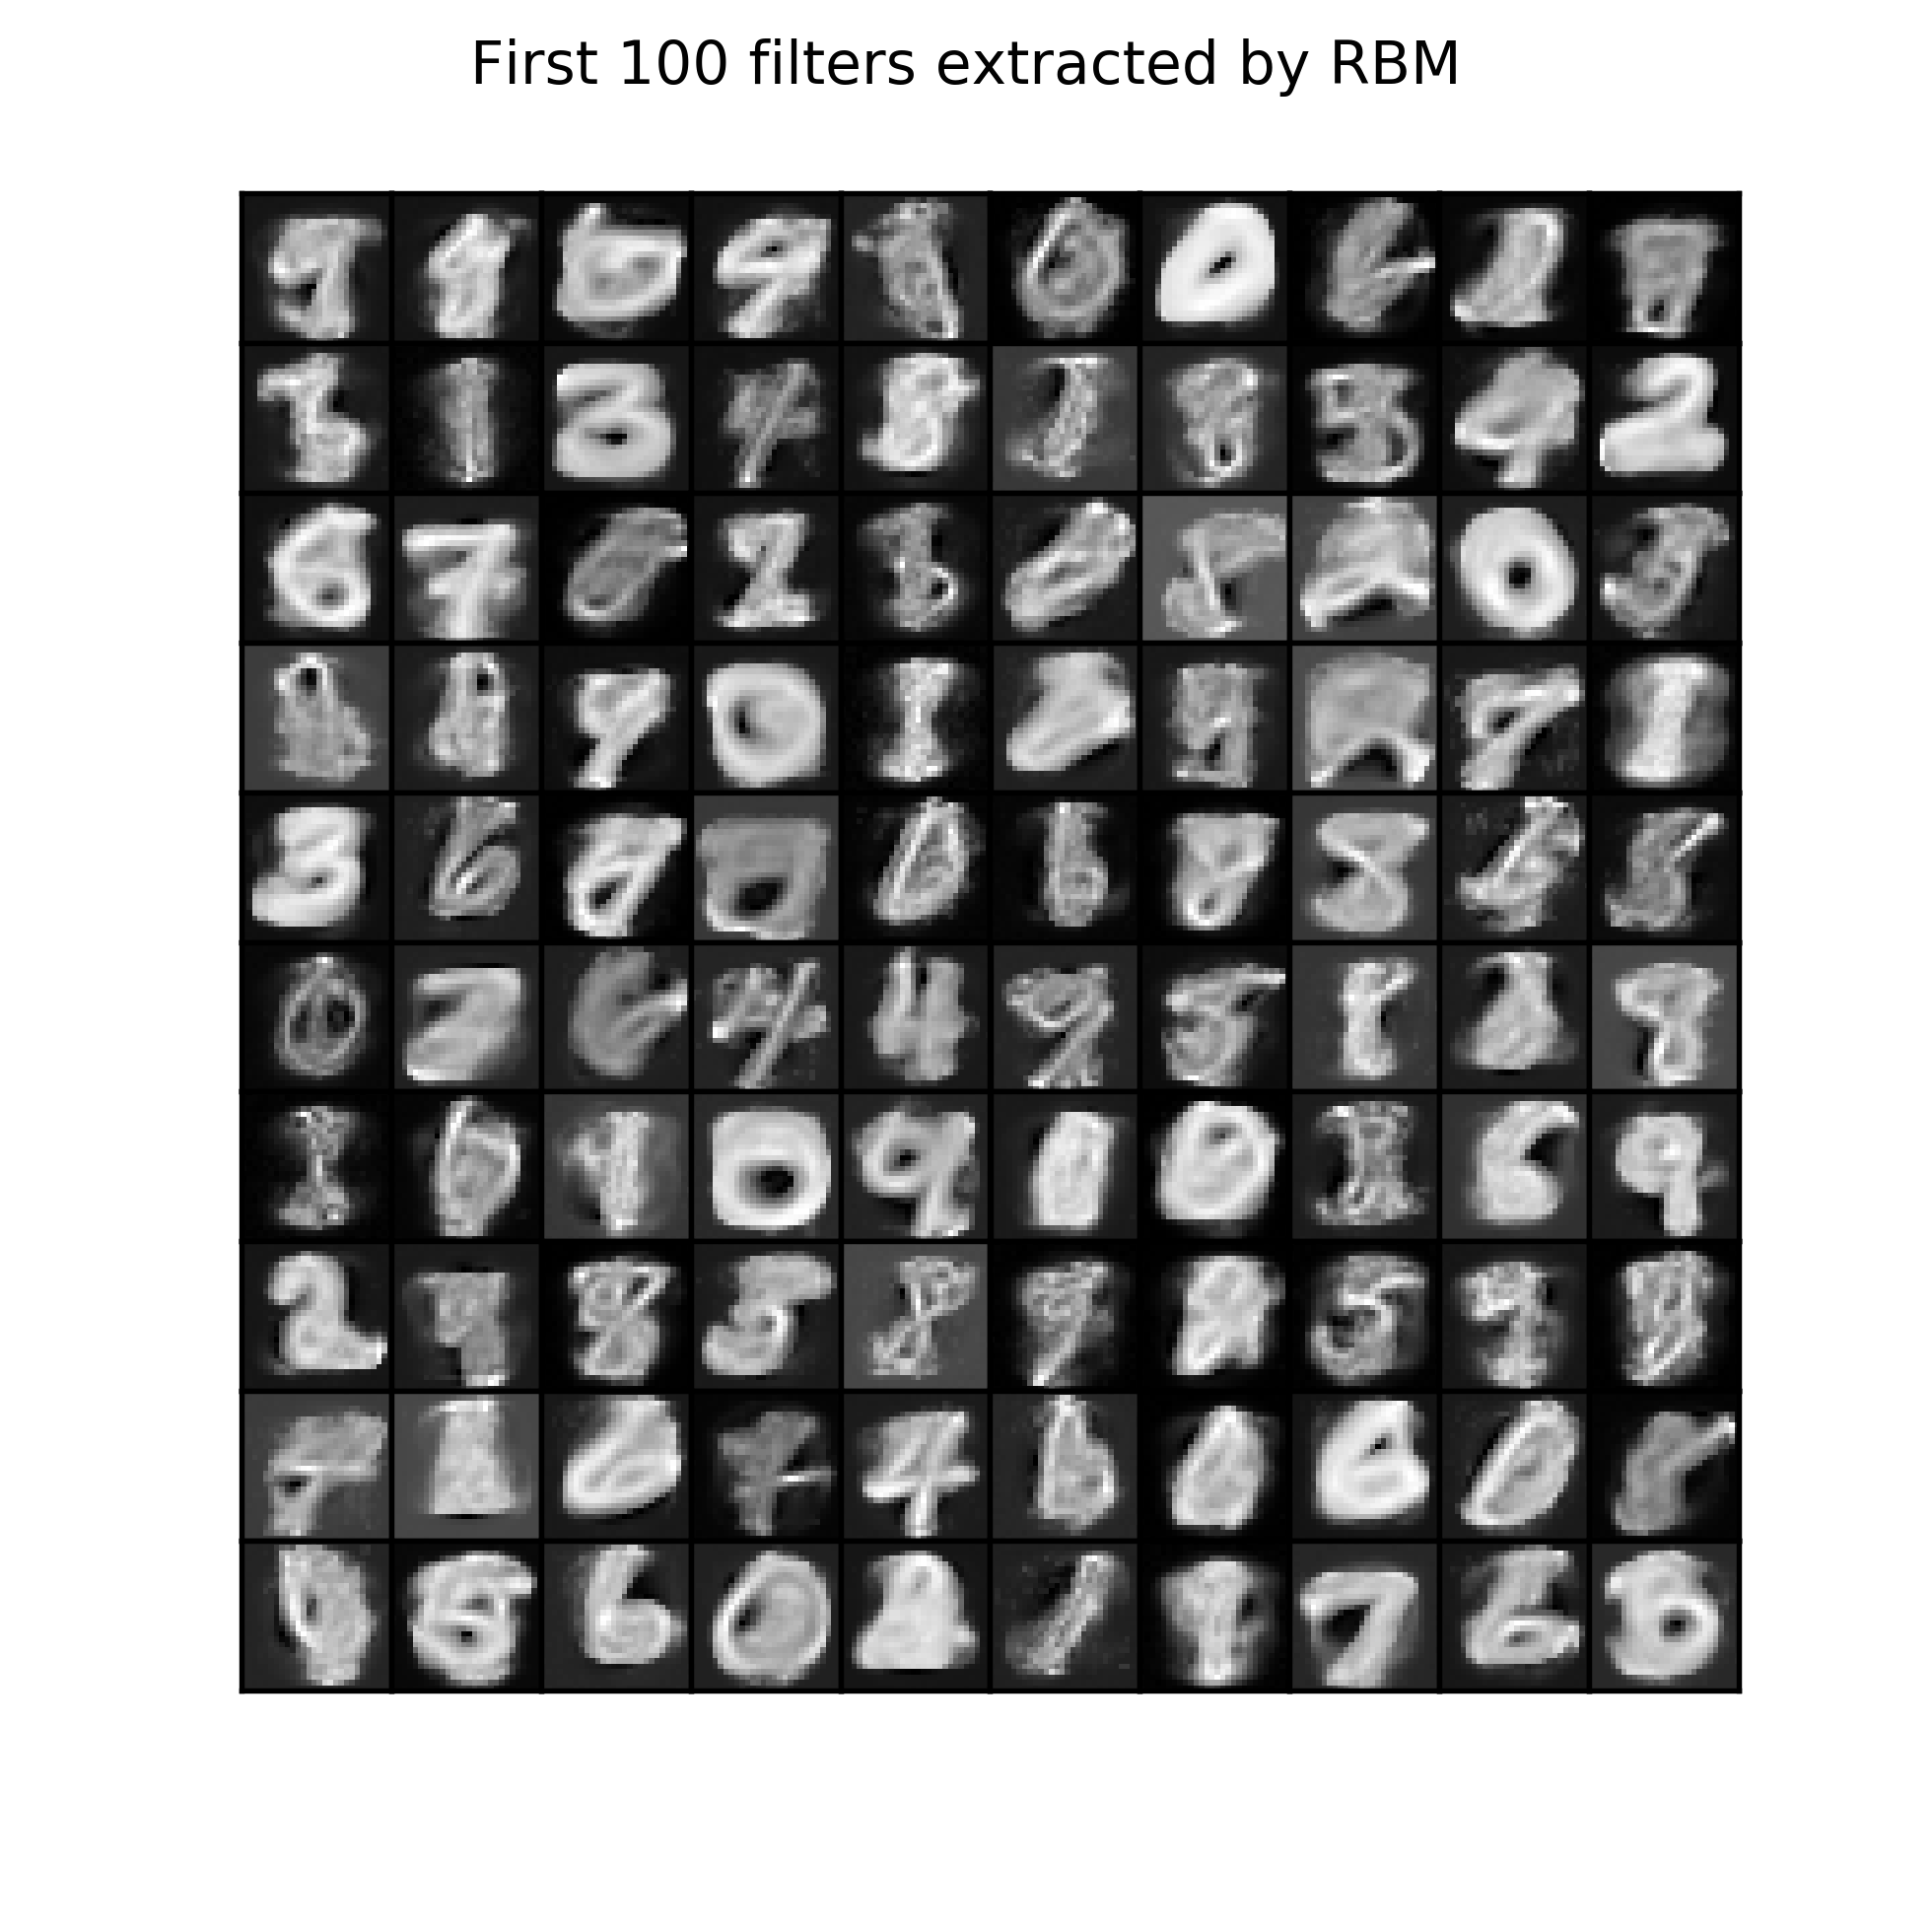
\includegraphics[width=.32\textwidth]{rbm-mnist/st_rbm_mnist_1e-3.png}

\medskip

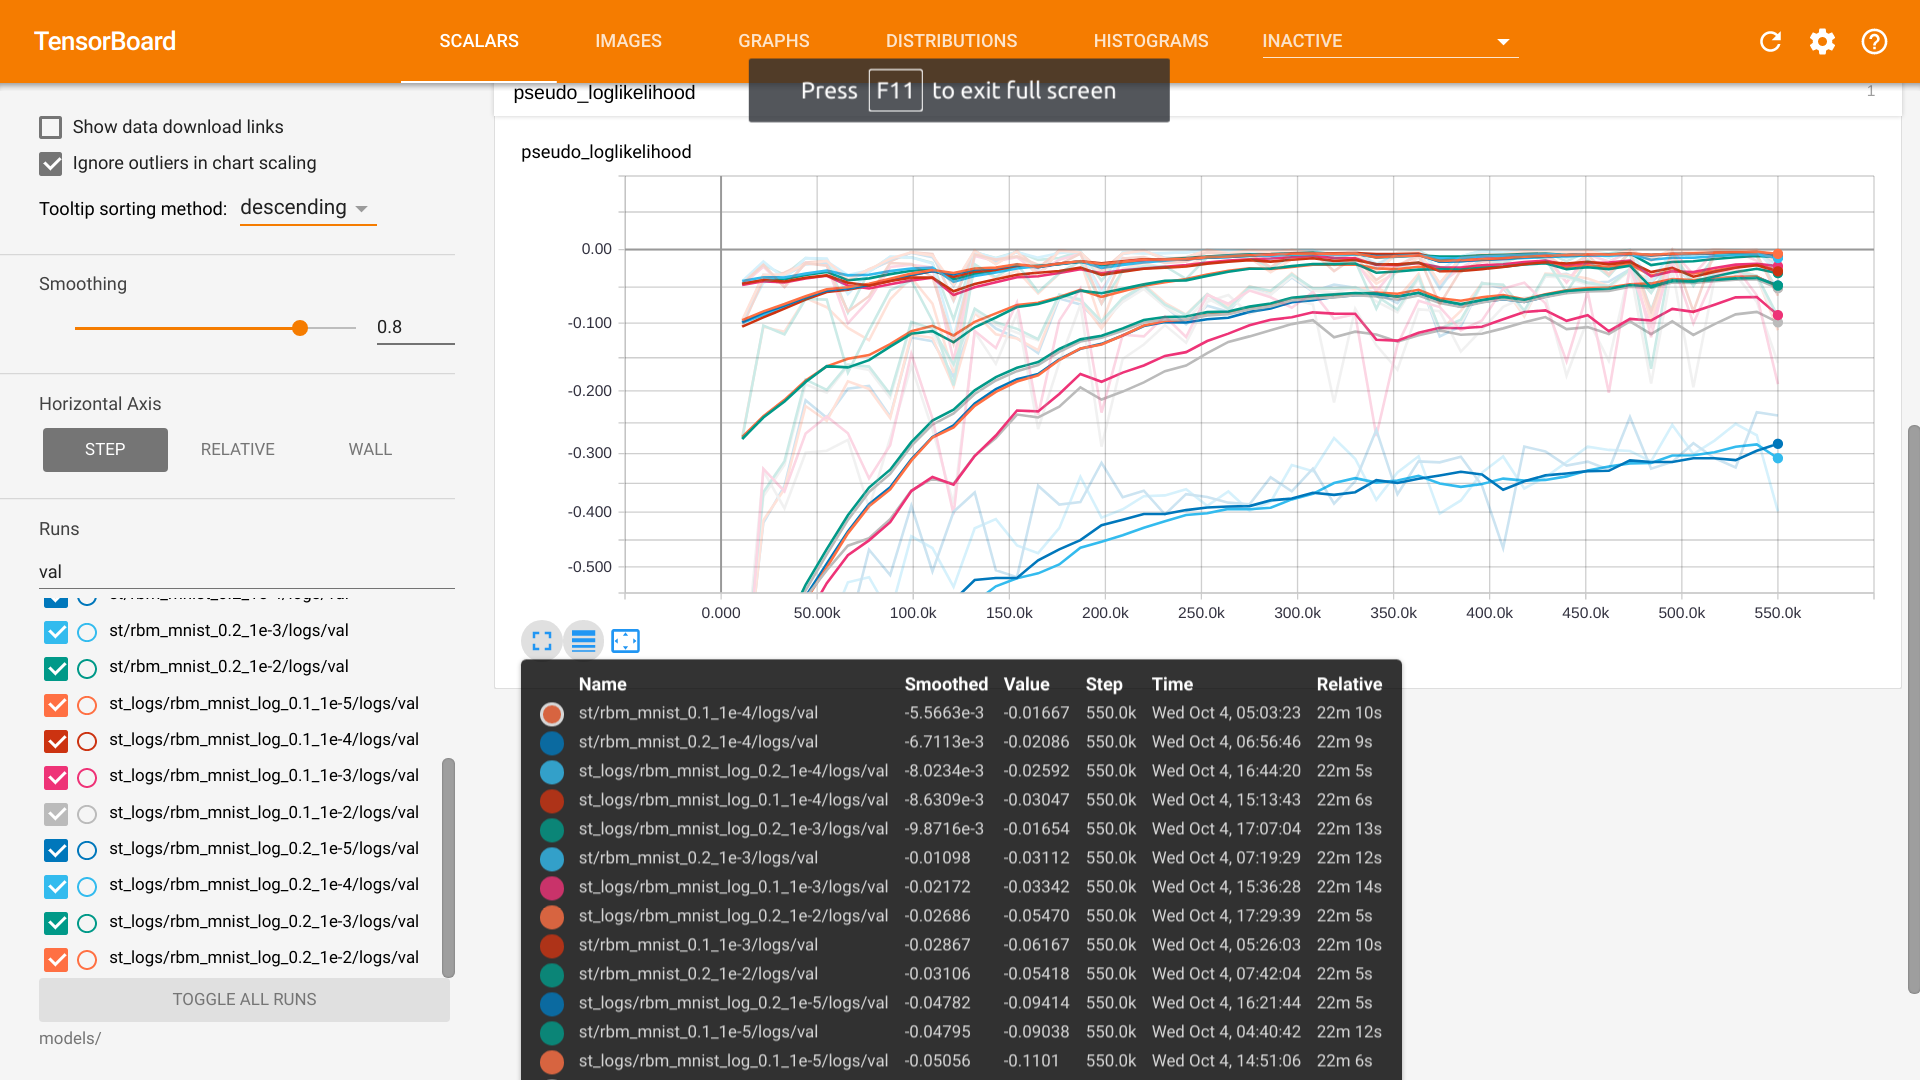
\includegraphics[width=.9\textwidth]{rbm-mnist/st_st_log_pll.png}
\caption{\emph{Top}: filters learned in the previous experiment as $\lambda$ increases (from top to bottom, from left to right). \emph{Bottom}: PLL of best models from previous experiment and ones with hidden biases initialized as $\log\l(\frac{t}{1-t}\r)$ for sparsity target $t$.}
\end{mdframed}
\end{figure*}

\clearpage

\begin{figure}[h]
\begin{mdframed}
\centering
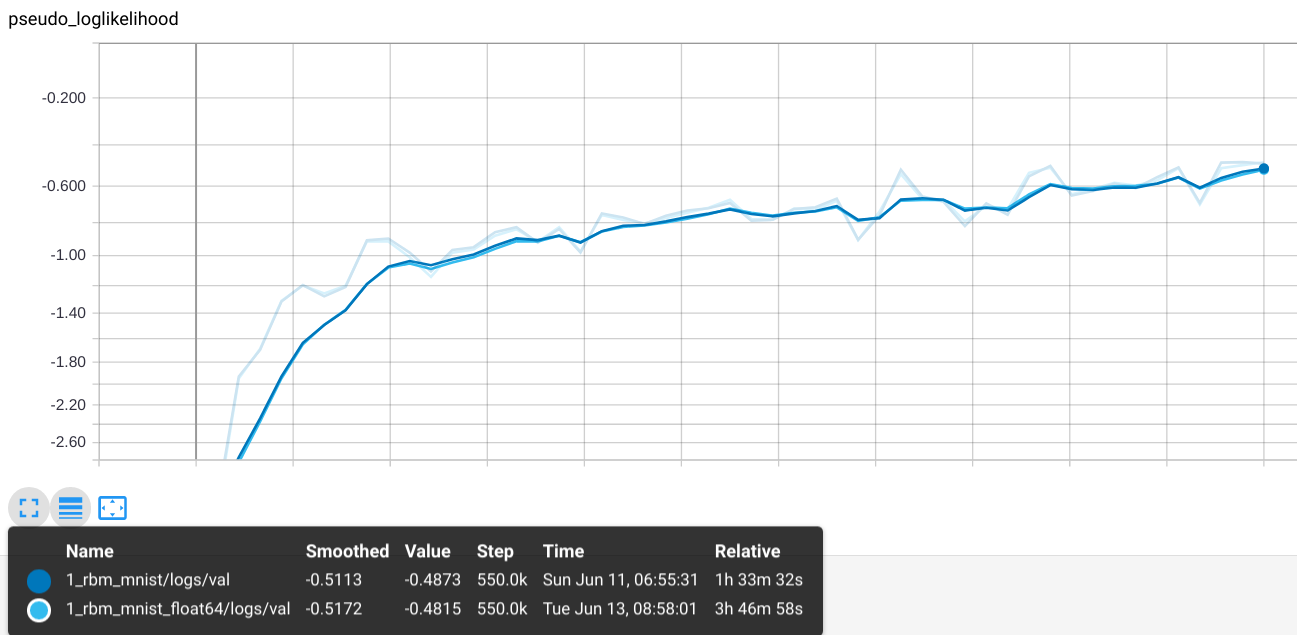
\includegraphics[width=5.8in]{rbm-mnist/float32_float64.png}
\\[1em]
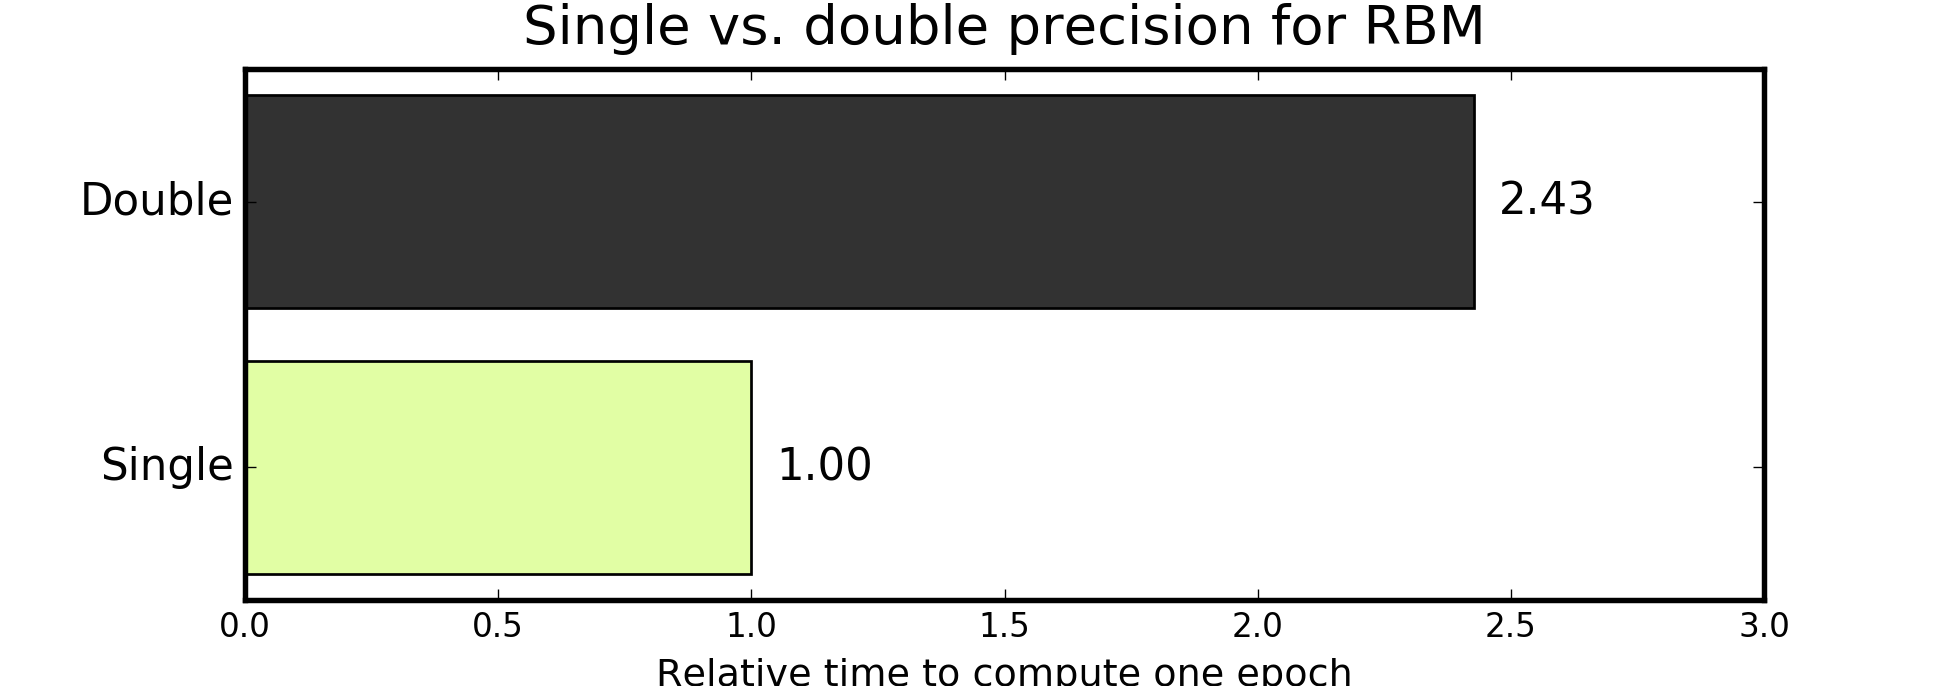
\includegraphics[width=3in]{rbm-mnist/rbm_speedup.png}
\\[1em]
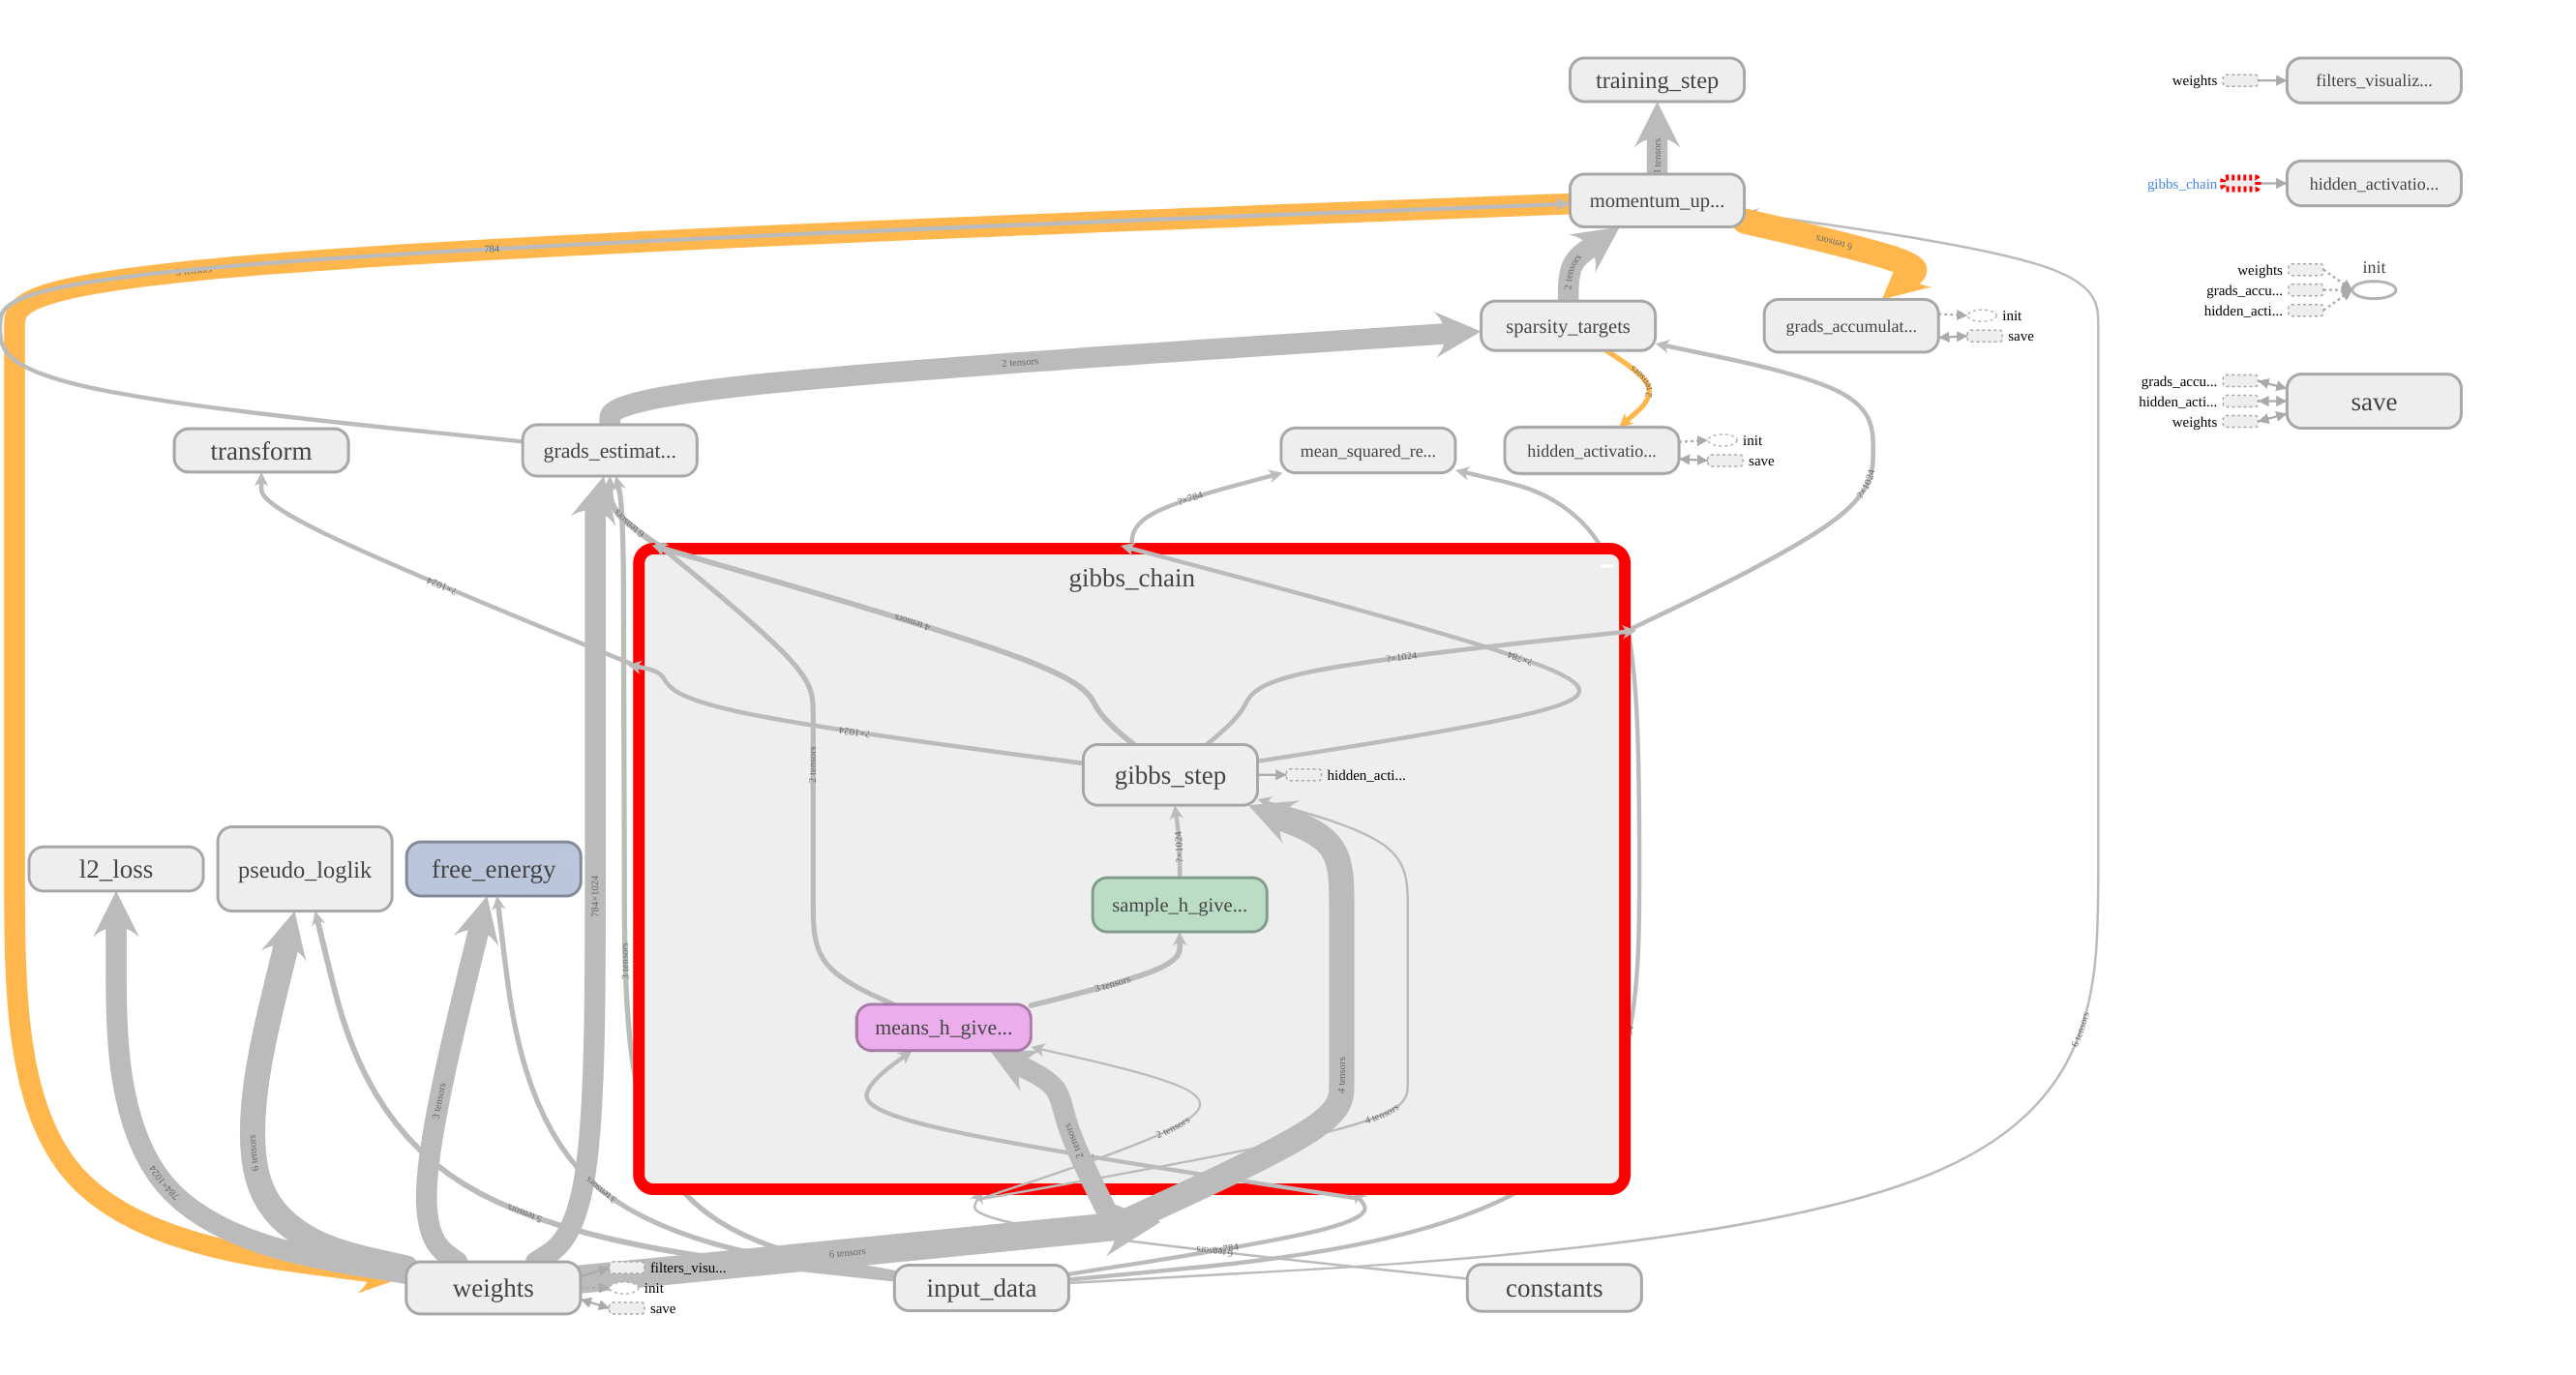
\includegraphics[width=5.6in]{rbm/tf_graph.png}
\caption{\emph{Top}: When single precision is used, the difference in performance is negligible compared to the double precision, training however is almost 2.5 times faster (pseudo log-lik is slightly more noisy at the beginning of training though). \emph{Bottom}: high-level computational graph for RBM.}
\end{mdframed}
\end{figure}

\clearpage

	\newpage
\section{Deep Boltzmann Machines \cite{salakhutdinov2013learning, salakhutdinov2009deep, goodfellow2016deep}}
\subsection{More efficient learning algorithm for general binary-binary BMs}
\subsubsection{PCD-k}
To recap:
\bg
\frac{1}{N}\sum_{n=1}^N\nabla_{\mb{W}}\log p(\mb{x}_n;\bs{\psi}) = \E_{\mb{v},\mb{h}\sim P_{\text{data}}(\mb{v},\mb{h};\bs{\psi})}\l[\mb{v}\mb{h}^T\r]-\E_{\mb{v},\mb{h}\sim P_{\text{model}}(\mb{v},\mb{h};\bs{\psi})}\l[\mb{v}\mb{h}^T\r]
\eg
and similar formulae for log-likelihood gradients w.r.t. $\mb{L},\mb{J},\mb{b},\mb{c}$, see (17).
\\[0.5em]
Now, instead of CD-k we use PCD-k (i.e. we keep one Markov chain without restarting its state between the updates), which falls into class of so-called \emph{Stochastic approximation procedures} (SAP) to estimate \tb{model's} expectations.
\\[1em]
Let $\bs{\psi}^t$ and $\mb{x}^t$ be the current model parameters and the state. Then $\mb{x}^t$ and $\bs{\psi}^t$ are updated sequentially as follows:
\begin{itemize}
	\item given $\mb{x}^t$, a new state $\mb{x}^{t+1}$ is sampled from a transition operator $T_{\bs{\psi}^t}(\mb{x}^{t+1}\leftarrow \mb{x}^t)$ that leaves $p(\cdot,\cdot;\bs{\psi}^t)$ invariant (which in our case is performing Gibbs sampling using equations (11) and (12) for $k$ steps);
	\item a new parameter $\bs{\psi}^{t+1}$ is then obtained by replacing the intractable model's expectation by the point estimate $\mb{x}^t$ (see also subsubsection 2.2.2 for whether to sample or use probabilities/means instead of sampling, and for which type of states)
\end{itemize}
In practice, we typically maintain a set of $P$ "persistent" sample "particles" $X^t=\{\mb{x}_1^t\ldots \mb{x}_{P}^t\}$ and use average over those particles.
\\[1em]
The intuition behind why this procedure works is the following: as the learning rate becomes sufficiently small compared with the mixing rate of the Markov chain, this "persistent" chain will always stay very close to the stationary distribution even if it is only run for a few MCMC updates per parameter update.
\\[1em]
Provided $\|\bs{\psi}^t\|$ is bounded and Markov chain, governed by a transition kernel $T_{\bs{\psi}^t}$ is ergodic (which is typically true in practice), and sequence of learning rates $\alpha_t$ satisfies $\sum_{t}\alpha_t=\infty$, $\sum_{t}\alpha_t^2<\infty$, this stochastic approximation procedure procedure is almost surely convergent to an asymptotically stable point.
\\
Note that in practice, $\alpha_t$ is not approached to zero, but rather to some small but positive constant $\varepsilon$ (e.g. $10^{-6}, 10^{-5}$).
\subsubsection{Variational learning}
Another approach is used to approximate \tb{data}-dependent expectations. We approximate true posterior over latent variables $p(\mb{h}|\mb{v};\bs{\psi})$ (which is intractable in general BM, tractable in RBM, but will be again intractable in DBM) by approximate posterior $q(\mb{h};\bs{\mu})$ and the variational parameters $\bs{\mu}$ are updated to follow the gradient of a \emph{lower bound on the log-likelihood}:
\\[1em]
In general:
\begin{empheq}[box={\mybox[1em][1em]}]{gather*}
\log p(\mb{v};\bs{\psi})=\int q(\mb{h};\bs{\mu})\log p(\mb{v};\bs{\psi})\mathrm{d}\mb{h}
=\int q(\mb{h};\bs{\mu})\log \frac{p(\mb{v},\mb{h};\bs{\psi})}{p(\mb{h}|\mb{v};\bs{\psi})}\mathrm{d}\mb{h}=\\
=\int q(\mb{h};\bs{\mu})\log \l(\frac{p(\mb{v},\mb{h};\bs{\psi})}{q(\mb{h};\bs{\mu})}\cdot \frac{q(\mb{h};\bs{\mu})}{p(\mb{h}|\mb{v};\bs{\psi})}\r)\mathrm{d}\mb{h}=\\
=\int q(\mb{h};\bs{\mu})\log p(\mb{v},\mb{h};\bs{\psi})\mathrm{d}\mb{h}
\underbrace{-\int q(\mb{h};\bs{\mu})\log q(\mb{h};\bs{\mu})\mathrm{d}\mb{h}}_{\mc{H}(q)}
+\underbrace{\int q(\mb{h};\bs{\mu})\log \frac{q(\mb{h};\bs{\mu})}{p(\mb{h}|\mb{v};\bs{\psi})}\mathrm{d}\mb{h}}_{D_{\text{KL}}(q(\mb{h};\bs{\mu}) \;\|\; p(\mb{h}|\mb{v};\bs{\psi}))\geq 0}\geq\\
\geq \int q(\mb{h};\bs{\mu})\log p(\mb{v},\mb{h};\bs{\psi})\mathrm{d}\mb{h} + \mc{H}(q) =: \mc{L}_{\text{ELBO}}(\bs{\mu}; \bs{\psi})
\end{empheq}
For Boltzmann Machine:
\begin{empheq}[box={\mybox[1em][1em]}]{gather*}
\text{\textbullet{} }[1]=\sum_{\mb{h}} q(\mb{h};\bs{\mu})\l[-E(\mb{v},\mb{h};\bs{\psi})=-\log Z(\bs{\psi}) \r]-\underbrace{\log Z(\bs{\psi})}_{=\text{ const w.r.t.}\bs{\mu}}\cdot\underbrace{\sum_{\mb{h}} q(\mb{h};\bs{\mu})}_{=1}+\\
+\sum_{\mb{h}} q(\mb{h};\bs{\mu})\l[\sum_{j<k}L_{jk}v_jv_k +\sum_{l<m}J_{lm}h_lh_m +\sum_{j,l}W_{jl}v_jh_l+\sum_jb_jv_j+\sum_lc_lh_l  \r]=\\
=\sum_{l<m}J_{lm}\E_{\mb{h}\sim q(\mb{h};\bs{\mu})}[h_lh_m]+\sum_{j,l}W_{jl}v_j\E_{\mb{h}\sim q(\mb{h};\bs{\mu})}[h_l]+\sum_lc_l\E_{\mb{h}\sim q(\mb{h};\bs{\mu})}[h_l]+\text{const}
\end{empheq}
For Boltzmann Machine and fully-factorizable $q(\mb{h};\bs{\mu})=\prod_l q(h_l;\mu_l), q(h_l=1;\mu_l)=\mu_l$ (\emph{mean-field} approach):
\begin{empheq}[box={\mybox[1em][1em]}]{gather*}
\text{\textbullet{} }[1]=\sum_{l<m}J_{lm}\mu_l\mu_m+\sum_{j,l}W_{jl}v_j\mu_l+\sum_lc_l\mu_l+\text{const}
\\
\text{\textbullet{} }[2]=\mc{H}(q)=-\sum_{\mb{h}}q(\mb{h};\bs{\mu})\log q(\mb{h};\bs{\mu})=-\sum_{\mb{h}}q(\mb{h};\bs{\mu})\sum_{j}\log q(h_j;\mu_j)=\\
=-\sum_j \sum_{h_j\in\{0,1\}}q(h_j;\mu_j)\log q(h_j;\mu_j) \underbrace{\sum_{\mb{h}_{-j}}q(\mb{h}_{-j};\bs{\mu}_{-j})}_{=1}=-\sum_j \mu_j\log \mu_j+(1-\mu_j)\log(1-\mu_j)
\end{empheq}
\bg
\boxed{\mc{L}_{\text{ELBO}}(\bs{\mu}; \bs{\psi})=\sum_{l<m}J_{lm}\mu_l\mu_m+\sum_{j,l}W_{jl}v_j\mu_l+\sum_lc_l\mu_l-\sum_j \mu_j\log \mu_j+(1-\mu_j)\log(1-\mu_j)+\text{C}}
\eg
Let us maximize (55) for $\bs{\mu}$ for fixed $\bs{\psi}$:
\begin{empheq}[box={\mybox[1em][1em]}]{gather*}
0 \doteq \frac{\partial}{\partial\mu_{i}}\mc{L}=\underbrace{\comment{$l=i$}\sum_{m>i}J_{im}\mu_m+\comment{$m=i$}\sum_{l<i}J_{li}\mu_l}_{=\comment{$J_{ij}=J_{ji},J_{ii}=0$}\sum_l J_{il}\mu_l}+\sum_{j}W_{ji}v_j+c_i
-\log \mu_i-1+\log(1-\mu_i)+1
\\
\Leftrightarrow
\\
\text{sigm}^{-1}(\mu_i)=\log\frac{\mu_i}{1-\mu_i}=\sum_{l<i}J_{li}\mu_l+\sum_{j}W_{ji}v_j+c_i
\end{empheq}
\bg
\boxed{\mu_i\leftarrow \text{sigm}\l(\sum_{l<i}J_{li}\mu_l+\sum_jW_{ji}v_j+c_i\r)}
\eg
Note that this is exactly the formula for (12) for computing $p(h_j=1|\mb{v},\mb{h}_{-i})$ in BM! So, updates of variational parameters can be computed using Gibbs sampler. This is not a coincidence, but the same holds if replace types of units, use RBM or even DBM (see below)!
\\[1em]
Note, that this variational approach cannot be used to approximate model-expectations because of minus sign in formulae (54),(17). This would cause variational learning to change the parameters so as to \emph{maximize} $D_{\text{KL}}(q(\mb{h};\bs{\mu}) \;\|\; p(\mb{h}|\mb{v};\bs{\psi}))$.
\\[0.5em]
The naive mean-field approach was chosen because:
\begin{itemize}
	\gooditem its convergence is usually fast;
	\gooditem it is unimodal.
\end{itemize}
Note that in general, we don't have to provide a parametric form of the approximating distribution beyond enforcing the independence assumptions. The variational approximation procedure is generally able to recover the functional form of the approximate distribution \cite{goodfellow2016deep}.

\subsection{Deep Boltzmann Machine}
Again assume unless specifically mentioned that DBM contains all binary units.
\subsubsection{High-level overview}
\textbullet{} DBM is a deep generative model, that consists of a layer of visible units and a series of layers of hidden units.
\begin{figure}[h]
\begin{mdframed}
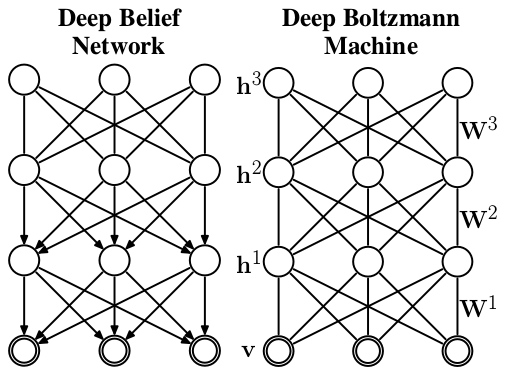
\includegraphics[scale=0.4]{img/dbn_dbm.png}
\centering
\caption{A three-layer Deep Belief Network and a three-layer Deep Boltzmann Machine.}
\label{fig:dbn_dbm}
\end{mdframed}
\end{figure}
In comparison to another deep generative model, DBN (which is hybrid, and has directed layers and one undirected), DBM is entirely undirected model, see Fig. \ref{fig:dbn_dbm}. DBN is trained using greedy, layer by layer training of corresponding RBMs (one bottom-top pass). At the same time, All parameters in DBM are learned \tb{jointly}, which greatly facilitates learning better generative models. Even though both models have a potential of learning series of internal representations that become increasingly complex, DBM's approximate bottom-top and top-bottom inference better propagate uncertainty $\Rightarrow$ deal more robustly with ambiguous inputs, than DBN.
\\
\textbullet{} Formally, suppose number of (hidden) layers $L=3$.
$$
\mb{v}\in\R^D, \mb{h}=\{\mb{h^{(1)}}, \mb{h^{(2)}}, \mb{h^{(3)}}\}, \mb{h^{(s)}}\in\R^{H_s}, s\in\{1,2,3\};
$$
Energy function:
\bg
E(\mb{v},\mb{h};\bs{\psi})=-\mb{v}^T\mb{W^{(1)}}\mb{h^{(1)}}-\mb{h^{(1)}}^T\mb{W^{(2)}}\mb{h^{(2)}}-\mb{h^{(2)}}^T\mb{W^{(3)}}\mb{h^{(3)}}-\mb{b}\cdot\mb{v}-\mb{c^{(1)}}\cdot\mb{h^{(1)}}-\mb{c^{(2)}}\cdot\mb{h^{(2)}}-\mb{c^{(3)}}\cdot\mb{h^{(3)}},
\eg
where $\bs{\psi}=\{\mb{W^{(1)}}, \mb{W^{(2)}}, \mb{W^{(3)}}, \mb{b}, \mb{c^{(1)}}, \mb{c^{(2)}}, \mb{c^{(3)}}\}$.
Probability that the model assign to a configuration $(\mb{v},\mb{h})$:
\bg
p(\mb{v},\mb{h};\bs{\psi})\;\propto\;\exp(-E(\mb{v},\mb{h};\bs{\psi}))
\eg
\\
\textbullet{} Now observe that conncections between units in the DBM are restricted in such a way, that unit from a layer depends only on the units from the \emph{neighboring} layers, and does not depend from other units in the same layer or in the layers beyond. This is a multi-layer generalization of RBM, and allows to compute probabilities of units on given the others efficiently. For instance,
\bg
p(h^{(1)}_j=1|\mb{v},\mb{h^{(2)}})=\text{sigm}\l(\sum_iW^{(1)}_{ij}v_i+\sum_iW^{(2)}_{jl}h_l^{(2)}+c_j^{(1)}\r)
\eg
Observe how this formula resembles formulae (21),(22). This is also easily generalizes to other layers and other types of layers:
\\[1em]
\noindent\fbox{%
	\parbox{\textwidth}{%
	To compute probability of unit being on given all the others, \tb{add} linear combinations of states of units from neighboring layers + bias and apply \tb{activation function of a unit} (e.g. sigmoid for binary, softmax for softmax/multinomial, affine for gaussian etc.).
	}%
}
\\[1em]
Note, however, that the distribution over \tb{all} hidden layers generally does not factorize because of interactions between layers. For instance, for $L=2$, $p(\mb{h}^{(1)},mb{h}^{(2)}|\mb{v};\bs{\psi})$ does not factorize due to interaction weights $\mb{W}^{(2)}$ between $\mb{h}^{(1)}$ and $\mb{h}^{(2)}$ which  render those variables mutually dependent.
\\
\textbullet{} Formulae for log-likelihood gradients are derived the same way as for RBM and have similar form. For instance:
\bg
\frac{1}{N}\sum_{n=1}^N\nabla_{\mb{W^{(2)}}}\log p(\mb{x}_n;\bs{\psi}) = \E_{\mb{h^{(1)}},\mb{h^{(2)}}\sim P_{\text{data}}(\mb{h^{(1)}},\mb{h^{(2)}};\bs{\psi})}\l[\mb{h^{(1)}}\mb{h^{(2)}}^T\r]-\E_{\mb{h^{(1)}},\mb{h^{(2)}}\sim P_{\text{model}}(\mb{h^{(1)}},\mb{h^{(2)}};\bs{\psi})}\l[\mb{h^{(1)}}\mb{h^{(2)}}^T\r]
\eg
\textbullet{} Finally, we apply new learning algortihms for BMs described in the previous subsection with fully-factorizable mean-field approach:
\bg
q(\mb{h};\bs{\mu})=\prod_j \prod_l \prod_m q(h_j^{(1)};\mu_j^{(1)}) \cdot q(h_l^{(2)};\mu_l^{(2)}) \cdot q(h_m^{(3)};\mu_m^{(3)})
\eg
Thanks to lack of intra-layer interaction makes it
possible to use fixed point equations (just like for general BM algorithm) to actually optimize the variational lower bound and find the true optimal mean field expectations.
\\
\textbullet{} Further we will use DBM with Gaussian visible units, Multinomial top-most layer hidden unist, and Bernoulli hidden units for intermediate layers. In this setting, again the learning algortihms remains the same, the difference is only in the way probabilities are computed, and samples are made.
\\
\textbullet{} One unfortunate property of DBMs is that sampling from them is relatively
difficult. DBNs only need to use MCMC sampling in their top pair of layers. The
other layers are used only at the end of the sampling process, in one efficient
ancestral sampling pass. To generate a sample from a DBM, it is necessary to
use MCMC across all layers, with every layer of the model participating in every
Markov chain transition.

\subsubsection{Gibbs sampling in DBMs}
\textbullet{} Similar to RBM, Gibbs sampling using equations (59) can be made in parallel thus allowing to perform block Gibbs sampling for each layer of units. In addition to that, as illustrated in Fig. \ref{fig:dbm_gibbs}, the DBM layers
can be organized into a bipartite graph, with odd layers on one side and even layers
on the other. This immediately implies that when we condition on the variables in
the even layer, the variables in the odd layers become conditionally independent. In conjuction with block Gibbs sampling for each layer, this allow to perform a Gibbs sampling in the whole DBM in \tb{only 2 iterations}, instead of $L + 1$, as one might naively think at first.
\\
\textbullet{} Good news that in TF no additional work need to be done beyond implementing block Gibbs sampling for each layer. Each independent branch in the computational graph should be executed in parallel.
\begin{figure}[h]
\begin{mdframed}
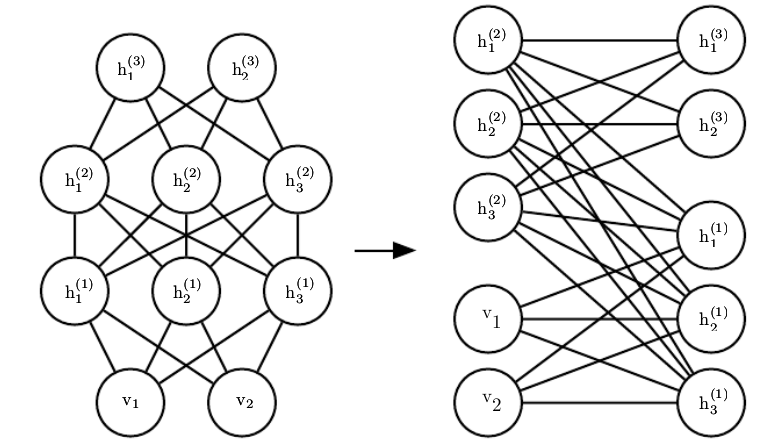
\includegraphics[scale=0.4]{img/dbm_gibbs.png}
\centering
\caption{A deep Boltzmann machine, re-arranged to reveal its bipartite graph structure.}
\label{fig:dbm_gibbs}
\end{mdframed}
\end{figure}
\textbullet{} Note that Contrastive Divergence algorithm is slow for DBMs because they do not allow efficient sampling of the hidden states given the visible units -- instead, CD would require burning in a Markov chain every time a new negative phase sample is needed.
\subsubsection{Greedy layerwise pretraining of DBMs}
DBM can be trained using the aforementioned learning algorithm from random initialization (typically the results are quite bad even on MNIST, see \cite{goodfellow2012joint, goodfellow2016deep}), but it works much better if weights are initialized sensibly. Greedy layerwise pretraining = learning procedure that consists of learning a stack of RBM's one layer at a time. After the stack is learned, the whole stack can be viewed as a single probabilistic model, called Deep Belief Net. Thus, pre-training for DBN is straightforward. In case of DBM though, a layer in the middle of the stack of RBMs is trained with only bottom-up input, but after the stack is combined to form DBM, the layer will have both bottom-up and top-down input. To account for this so-called \emph{evidence double counting problem} \cite{salakhutdinov2009deep, goodfellow2016deep}, Fig. \ref{fig:dbm_pretraining}, two modifications are required:
\begin{figure}[h]
\begin{mdframed}
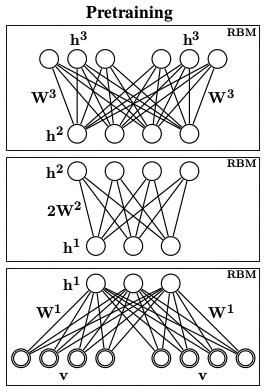
\includegraphics[width=1.5in]{img/dbm_pretraining2.png}
\quad
\quad
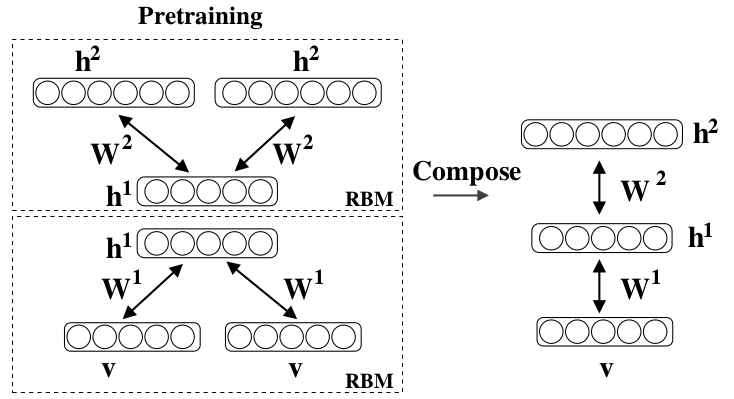
\includegraphics[width=3.5in]{img/dbm_pretraining.png}
\centering
\caption{Pre-training consists of learning a stack of modified RBMs, that are then composed to create a DBM.}
\label{fig:dbm_pretraining}
\end{mdframed}
\end{figure}
\begin{itemize}
	\item bottom RBM should be trained using two "copies" of each visible unit and the weights tied to be equal between these two copies ($\cong$ simply double the total input to hidden layer during upward pass); similarly, top RBM should be trained with two copies of topmost layer. Training of all intermediate RBMs if there are any, should not be modified.
	\item the weights of all intermediate RBMs though, should be divided by 2 before inserting into DBM
\end{itemize}
\begin{figure}[h]
\begin{mdframed}
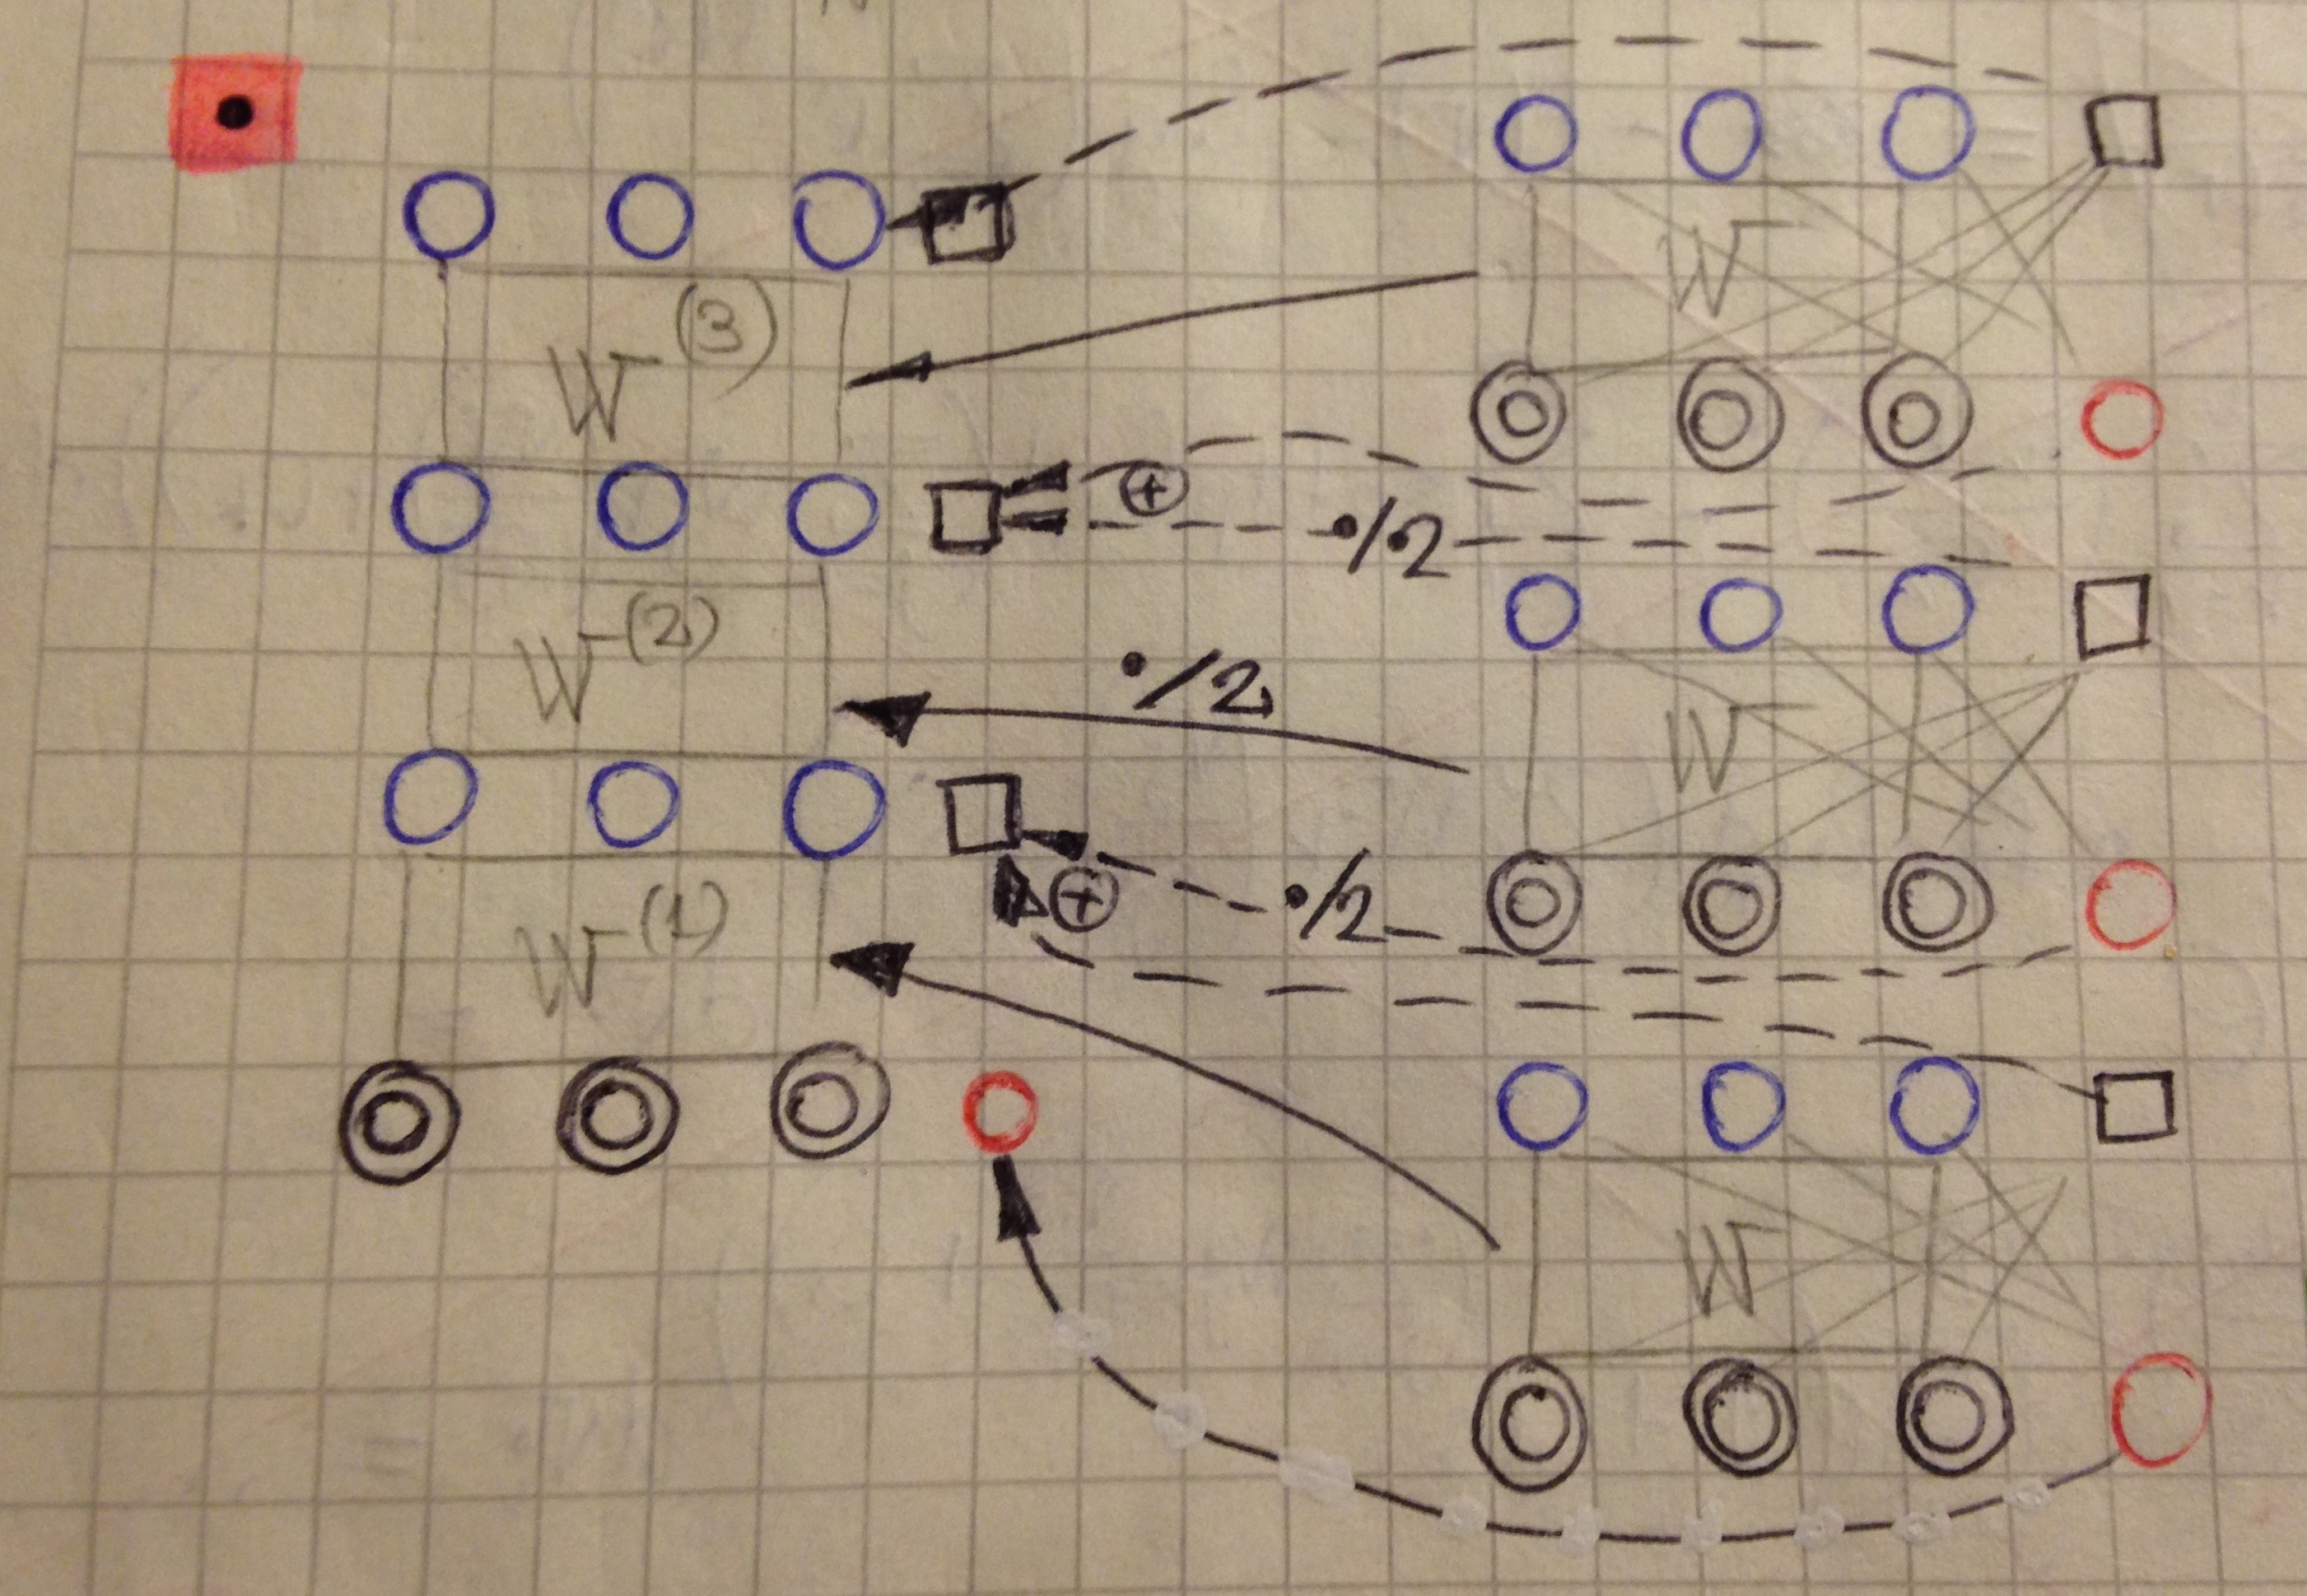
\includegraphics[scale=0.08]{dbm/dbm_init.jpg}
\centering
\caption{A more detailed scheme how to initialize 3-layer DBM from learned stack or RBMs, including biases. Black circles -- visible units, blue -- hidden units, red circel -- visible bias, black square -- hidden bias. Biases can be summed or averaged.}
\label{fig:dbm_init}
\end{mdframed}
\end{figure}

\subsubsection{Joint training of DBMs}
Classic DBMs require greedy unsupervised pretraining, and to perform classification
well, require a separate MLP-based classifier on top of the hidden features they
extract. It is hard to track performance
during training because we cannot evaluate properties of the full DBM while
training the first RBM. Software implementations
of DBMs need to have many different components for CD training of individual
RBMs, PCD training of the full DBM, and training based on back-propagation
through the MLP. Finally, the MLP on top of the Boltzmann machine loses many
of the advantages of the Boltzmann machine probabilistic model, such as being
able to perform inference when some input values are missing.
\\
There are two main ways to resolve the joint training problem of the deep
Boltzmann machine: \tb{multi-prediction DBMs}\cite{goodfellow2013multi}, which is currently beyond the scope of this project, and the \tb{centering trick} \cite{montavon2012deep}, which reparametrizes the model in order to make the Hessian of the cost function better-conditioned at the beginning of the learning process. More specifically, if we consider energy function of generalized Boltzmann Machine (BM, RBM, DBM can all be represented by appropriate choice of $\mb{x}$ -- states, $\mb{U}$ -- weights, $\mb{a}$ -- biases):
\bg
E(\mb{x};\bs{\psi})=-\mb{x}^T \mb{U}\mb{x}-\mb{a}\cdot\mb{x}
\eg
Then the idea of centering trick is simply to reparameterize this energy function as 
\bg
E(\mb{x};\bs{\psi})=-(\mb{x}-\bs{\beta})^T \mb{U}(\mb{x}-\bs{\beta})-\mb{a}\cdot(\mb{x}-\bs{\beta})
\eg
Where new hyperparameter vector $\bs{\beta}$ is chosen to be $\mb{x}-\bs{\beta}\approx \mb{0}$ at the beginning of training. This does not change the set of probability distributions that the model can represent, but it does change the learning dynamics so much, that it is actually possible to train DBM from random initialization w/o pre-training and achieve sensible results. However, in \cite{goodfellow2013multi} they say when DBM is trained using centering trick, they have never shown to have good classification performance, if this was the primary goal.

\subsubsection{Annealed importance sampling \cite{salakhutdinov2008, salakhutdinov2009deep, hinton2012better, upadhya2015empirical}}
Let $p_A(\mb{x})=\frac{p^*_A(\mb{x})}{\mc{Z}_A}$ be simple proposal distribution from which we can sample easily, and $p_{B}(\mb{x})=\frac{p^*_B(\mb{x})}{\mc{Z}_B}$ our complex target distribution. We also have to make sure $p_B \ll p_A$, which is easy in our case, since we can always choose $p_A$ to be uniform pmf, which dominates every other probability mass function on discrete units (of finite cardinality).
\\[0.5em]
\u{(Classical) Importance Sampling}
\\
The ratio of partition functions can be estimated as follows
\bg
\frac{\mc{Z}_B}{\mc{Z}_A}=\frac{p^*_B(\mb{x})}{p^*_A(\mb{x})}=\sum_{\mb{x}}\frac{p^*_B(\mb{x})}{p^*_A(\mb{x})} p_A(\mb{x})=\E_{\mb{x}\sim p_A}\l[\frac{p^*_B(\mb{x})}{p^*_A(\mb{x})} \r] \approx \frac{1}{N}\sum_{i=1}^N \frac{p^*_B(\mb{x}_i)}{p^*_A(\mb{x}_i)}
\eg
The problem is when $p_A$ and $p_B$ are very different, as in our case, this estimator is very poor: its variance is very large, possibly infinite.
\\[0.5em]
\u{Annealed Importance Sampling}
\\
To handle this issue, we define sequence of probability mass functions $\l(p_m\r)_{m=0:M}$ such that $p_0 = p_A$ and $p_M = p_B$, and for which we know unnormalized probabilities $p_m^*$, which typically are mixtures of target and proposal:
\bg
p_m(\mb{x})=p_B(\mb{x})^{\beta_m}\cdot p_A(\mb{x})^{1-\beta_m}, \beta_m=\frac{m}{M}
\eg
Also, in order not to sample from $p_s$ we also need sequence of transition operators $\l(T_i(\mb{x}_{i + 1} \leftarrow \mb{x}_i)\r)_{i=1:M-1}$ each that leaves the corresponding $p_i$ invariant. The importance weight can then be computed as
\bg
\omega_{\text{AIS}} \leftarrow \prod_{m=1}^M \frac{p_m^*(\mb{x}_m)}{p_{m-1}^*(\mb{x}_m)}
\eg
where $\mb{x}_1 \sim p_0=p_A;\; \mb{x}_2 \sim T_1(\mb{x}_2 \leftarrow \mb{x}_1);\; \ldots \; \mb{x}_M \sim T_{M-1}(\mb{x}_M \leftarrow \mb{x}_{M-1})$.
The ratio of partition functions can then be estimated as average over many AIS runs:
\bg
\frac{\mc{Z}_B}{\mc{Z}_A}=\frac{\mc{Z}_M}{\mc{Z}_0}\approx \frac{1}{L}\sum_{l=1}^L \omega_{\text{AIS}}^{(l)}
\eg
Notice also that we don't need to compute partition functions of any of the intermediate distributions.
\\
\tb{Note}: to avoid numerical problems and overflow errors (partition functions are very large numbers even for very moderate sized BM), all computations are performed in $\log$-domain, as usual.
\\[0.5em]
\u{Annealed Importance Sampling for 2-layer Bernoulli BM}
\\
It turns out that we can reduce state space of AIS to only hidden units in first layer $\mb{x}=\{\mb{h}^{(1)}\}$ by explicitly summing out visible and top-most layer hidden units:
\begin{empheq}[box={\mybox[1em][1em]}]{align*}
\log p^*\l(\mb{h}^{(1)}\r) &= \log \sum_{\mb{v},\mb{\mb{h}^{(2)}}} p^*\l(\mb{v}, \mb{h}^{(1)}, \mb{h}^{(2)}\r)=
\\
&= \log \sum_{\mb{v},\mb{\mb{h}^{(2)}}} \exp \l( \mb{v}^T\mb{W}^{(1)}\mb{h}^{(1)} +
\mb{h}^{(1)^T}\mb{W}^{(2)}\mb{h}^{(2)} + \mb{b}\cdot\mb{v} + \mb{c}^{(1)}\cdot\mb{h}^{(1)} + \mb{c}^{(2)}\cdot\mb{h}^{(2)} \r)
\\
&= \mb{c}^{(1)}\cdot\mb{h}^{(1)} + \log\l[ \sum_{\mb{v}}\exp\l( \mb{v}^T\mb{W}^{(1)}\mb{h}^{(1)} + \mb{b}\cdot\mb{v} \r)\sum_{\mb{h}^{(2)}} \exp\l( \mb{h}^{(1)^T}\mb{W}^{(2)}\mb{h}^{(2)} + \mb{c}^{(2)}\cdot\mb{h}^{(2)} \r) \r]
\\
&= \mb{c}^{(1)}\cdot\mb{h}^{(1)} + \sum_i^V \text{softplus}\l(\sum_j^{H_1} W_{ij}^{(1)}h_j^{(1)}+b_i \r) + \sum_k^{H_2} \text{softplus}\l(\sum_j^{H_1} W_{jk}^{(2)}h_k^{(2)}+c_k^{(2)} \r)
\end{empheq}
\bg
\boxed{\log p^*\l(\mb{h}^{(1)}\r)=\mb{c}^{(1)}\cdot\mb{h}^{(1)} + \sum_i^V \text{softplus}\l(\sum_j^{H_1} W_{ij}^{(1)}h_j^{(1)}+b_i \r) + \sum_k^{H_2} \text{softplus}\l(\sum_j^{H_1} W_{jk}^{(2)}h_k^{(2)}+c_k^{(2)} \r)}
\eg
From this we can easily derive equation for $\log p_{\textcolor{red}{m}}^*$ by simply scaling all weights by $\beta_m$:
\begin{equation}
\begin{aligned}
\log p_{\textcolor{red}{m}}^*\l(\mb{h}^{(1)}\r) =
\textcolor{red}{\beta_m}\mb{c}^{(1)}\cdot\mb{h}^{(1)} + \sum_i^V \text{softplus}\l(\textcolor{red}{\beta_m}\cdot\l(\sum_j^{H_1} W_{ij}^{(1)}h_j^{(1)}+b_i \r)\r) +
\\
+ \sum_k^{H_2} \text{softplus}\l(\textcolor{red}{\beta_m}\cdot\l(\sum_j^{H_1} W_{jk}^{(2)}h_k^{(2)}+c_k^{(2)} \r)\r)
\end{aligned}
\end{equation}
When $\beta_m=1$ we obtain target distribution, when $\beta_m=0$ we obtain uniform distribution:
\bg
\log p_0^*\l(\mb{h}^{(1)}\r) \equiv 0+\sum_i^V \text{softplus}(0) + \sum_k^{H_2} \text{softplus}(0)=(V+H_2)\log 2
\eg
thus $ \log \mc{Z}_0=(V+H_1+H_2)\log 2$.
\\[1em]
Thus we gradually increase "inverse temperature" $\beta$ from 0 to 1 and can estimate partition function using procedure described above. Staring from randomly initialized $\mb{h}^{(1)}$, we apply sequence of transition operators $T_i$ which are simply alternating Gibbs sampler with weights scaled by $\beta_i$.
\\[1em]
We can do the same for different types of units and larger number of layers. In the latter case we can again analytically sum out visible and top-most hidden units.
\\[0.5em]
\u{Variational lower-bound}
\\
Having estimate of partition function $\t{\mc{Z}}$, we can estimate variational lower-bound on test vector $\mb{v}^*$ as follows
\begin{equation}
\begin{aligned}
\log p(\mathbf{v}^{*};\boldsymbol{\psi})\geq\;&-\sum_{\mathbf{h}} q(\mathbf{h};\boldsymbol{\mu})E(\mathbf{v}^{*}, \mathbf{h};\boldsymbol{\psi})+\mathcal{H}(\boldsymbol{\mu})-\log\mathcal{Z}(\boldsymbol{\psi})
\\
=\;& \mathbf{v}^{*^{T}}\mathbf{W}^{(1)}\boldsymbol{\mu}_{\mathbf{v}^*}^{(1)}+\boldsymbol{\mu}_{\mathbf{v}^*}^{(1)^{T}}\mathbf{W}^{(2)}\boldsymbol{\mu}_{\mathbf{v}^*}^{(2)}+\mathbf{b}\cdot\mathbf{v}^{*}+\mathbf{c}^{(1)}\cdot\boldsymbol{\mu}_{\mathbf{v}^*}^{(1)}+\mathbf{c}^{(2)}\cdot\boldsymbol{\mu}_{\mathbf{v}^*}^{(2)}+\mathcal{H}(\boldsymbol{\mu}_{\mathbf{v}^*})-\log\mathcal{Z}(\boldsymbol{\psi})
\\
\approx\;& \mathbf{v}^{*^{T}}\mathbf{W}^{(1)}\boldsymbol{\mu}_{\mathbf{v}^*}^{(1)}+\boldsymbol{\mu}_{\mathbf{v}^*}^{(1)^{T}}\mathbf{W}^{(2)}\boldsymbol{\mu}_{\mathbf{v}^*}^{(2)}+\mathbf{b}\cdot\mathbf{v}^{*}+\mathbf{c}^{(1)}\cdot\boldsymbol{\mu}_{\mathbf{v}^*}^{(1)}+\mathbf{c}^{(2)}\cdot\boldsymbol{\mu}_{\mathbf{v}^*}^{(2)}+\mathcal{H}(\boldsymbol{\mu}_{\mathbf{v}^*})-\log\widehat{\mathcal{Z}}
\end{aligned}
\end{equation}
where $\bs{\mu}_{\mathbf{v}^*}$ are variational parameters obtained by running fixed-point equations using Gibbs sampler unitl convergence with visible units clamped to $\mathbf{v}^*$.
\\[1em]
One can also estimate true log-probability using AIS by clamping visible units to test example (estimating log-probability for one test example is computationally equivalent to estimating a partition function).

\subsubsection{Additional facts}
\textbullet{} In \cite{goodfellow2016deep} they say that obtaining sota results with DBM requires an additional partial mean field in negative phase, more details in \cite{goodfellow2013multi}.
\\
\textbullet{} The inference can further be accelerated using separate \emph{recognition model}, see \cite{salakhutdinov2010efficient} for details.
\\
\textbullet{} DBMs were developed after DBNs. Compared to DBNs, the posterior distribution $p(\mb{h}|\mb{v})$ is simpler for DBMs. Somewhat counterintuitively, the simplicity of this posterior distribution allows richer approximations of the posterior \cite{goodfellow2016deep}
\\
\textbullet{} The use of proper mean field allows the approximate inference procedure for DBMs to capture the influence of top-down feedback interactions. This makes
DBMs interesting from the point of view of neuroscience, because the human brain
is known to use many top-down feedback connections\cite{goodfellow2016deep}.
\\
\textbullet{} In \cite{goodfellow2013joint} they observe that energy function $E(\mb{v},\mb{h};\bs{\psi})$ inevitably induces some prior $p(\mb{h};\bs{\psi})$ that is not motivated by the structure of any kind of data. The role of deeper layers in DBM is simply to provide a better prior on the first layer hidden units.

\clearpage
\begin{figure}[h]
\begin{mdframed}
\centering
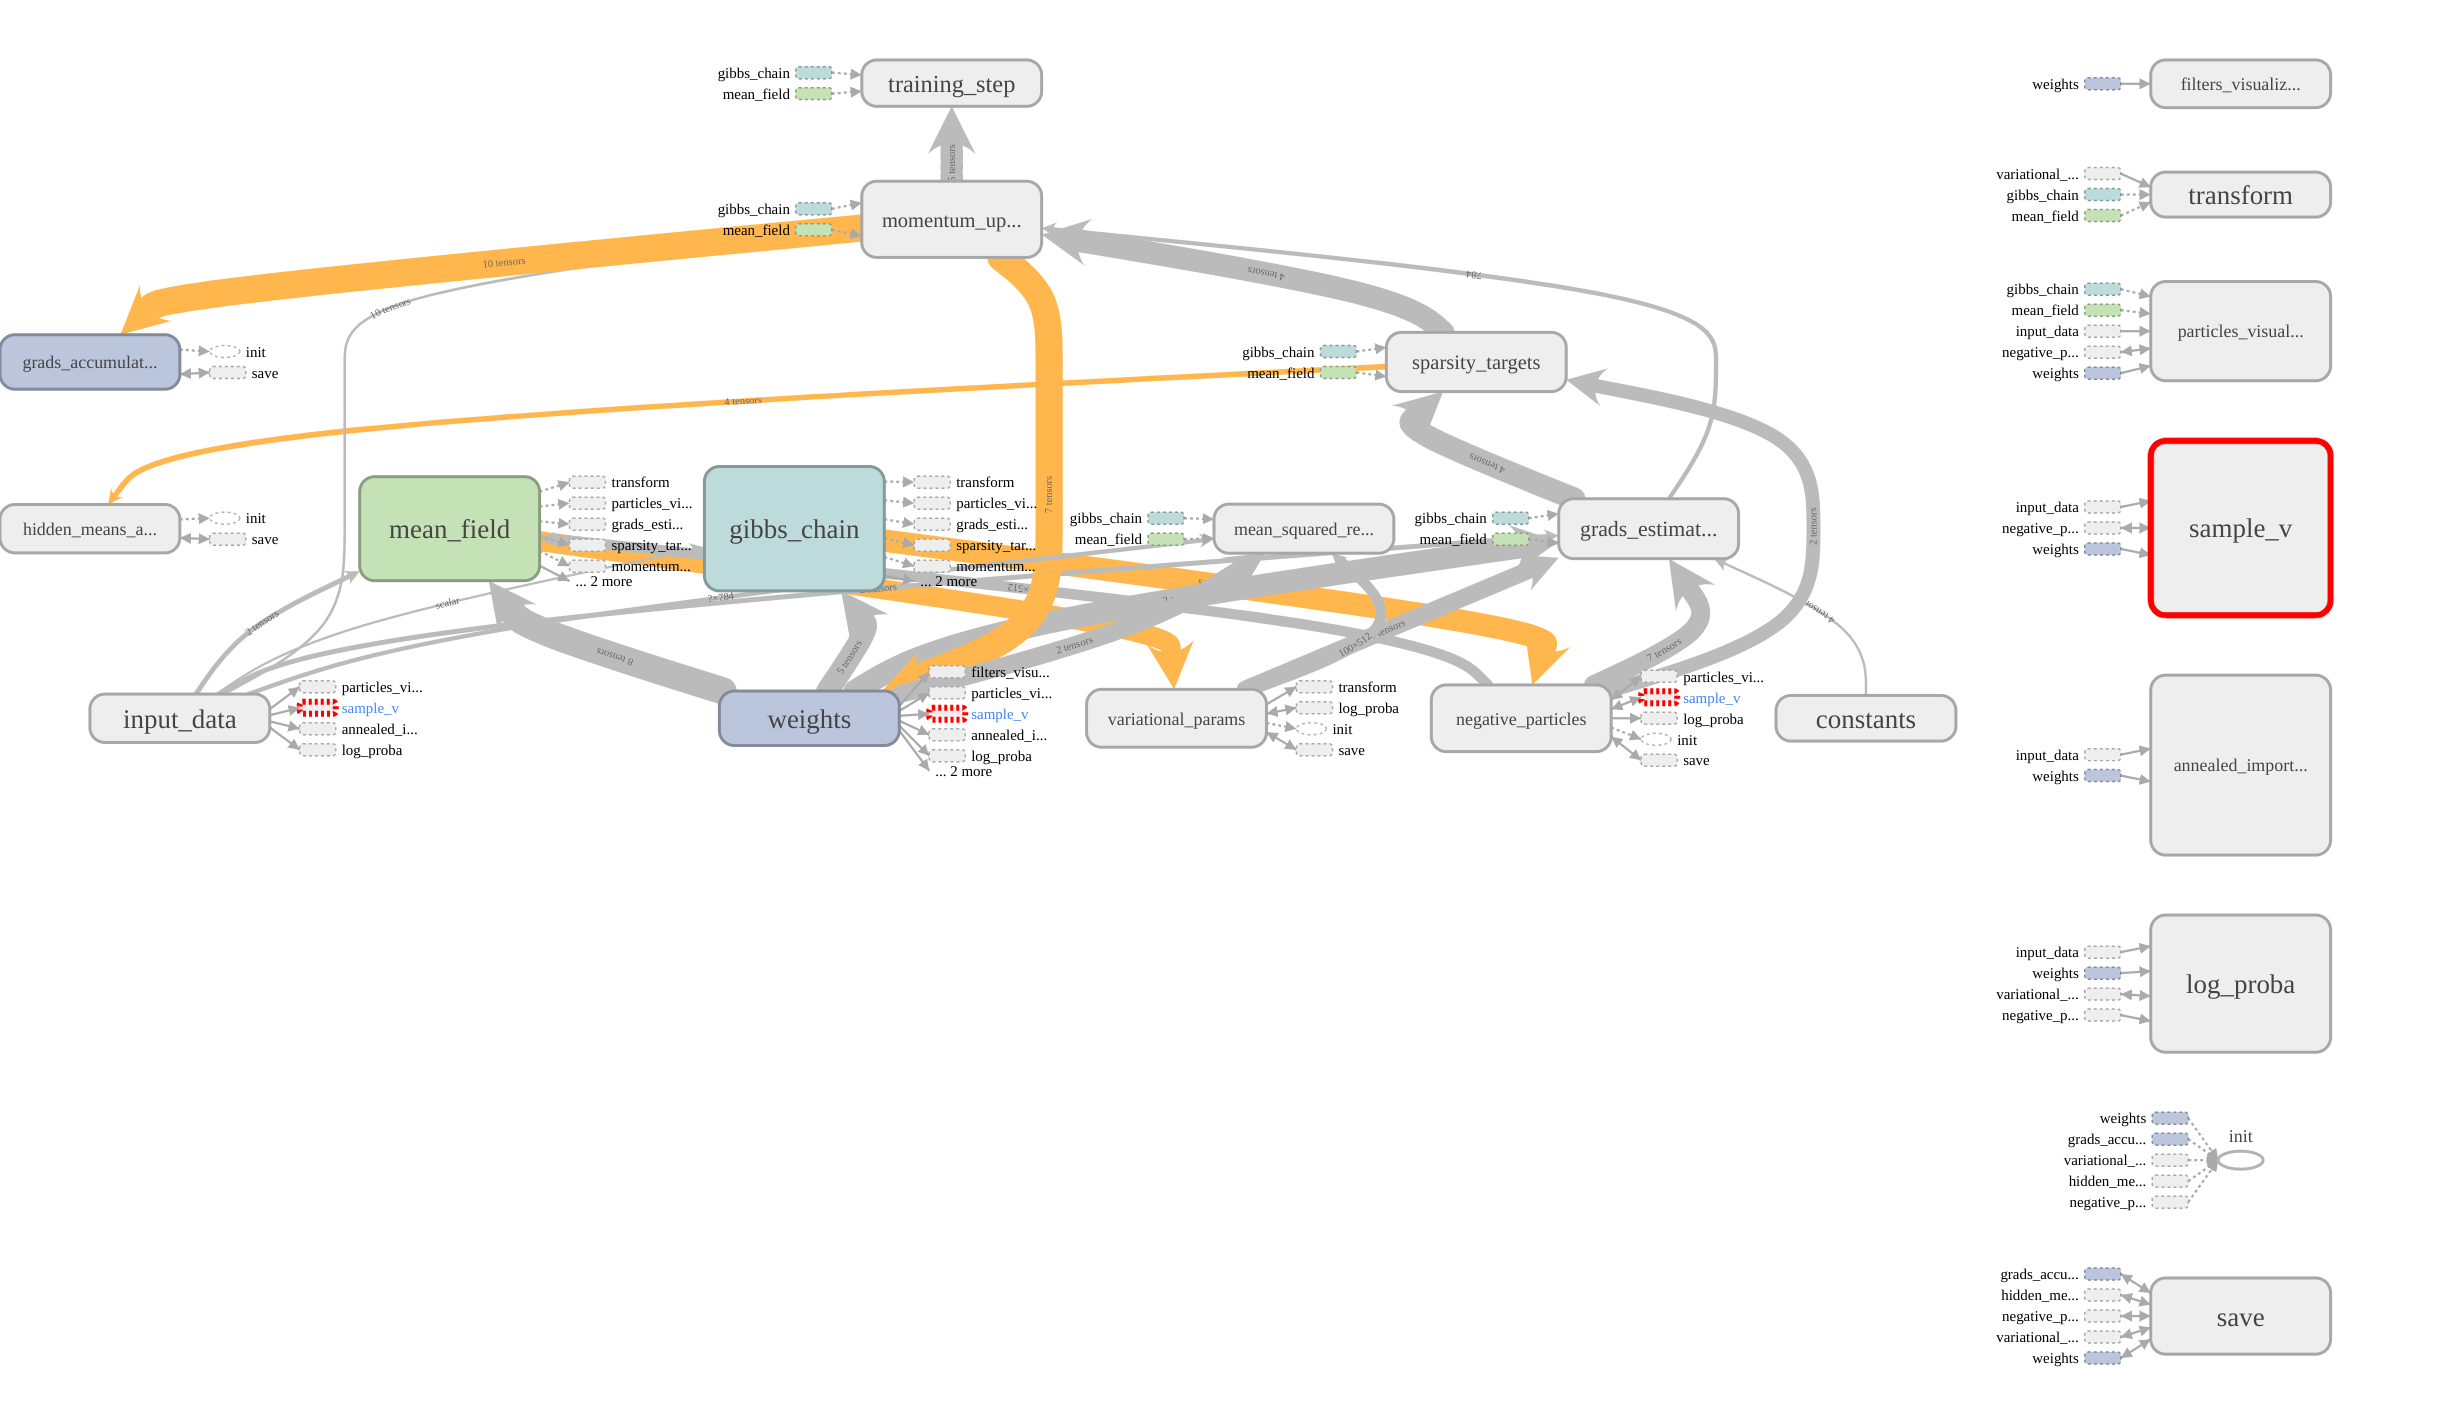
\includegraphics[width=6.4in]{dbm/tf_graph.png}
\caption{High-level computational graph for DBM model.}
\end{mdframed}
\end{figure}

	\newpage
\section{DBM experiments}
\subsection{Experiments on MNIST}
\subsubsection{Before sparsity targets, AIS}
Architecture and hyperparameters initially were similar to those of \cite{dbm_code}, however, I observe that learning rate should be smaller (eventually I used exactly 1 order of magnitude smaller starting learning rate).
\clearpage

\begin{figure}[h]
\begin{mdframed}
\centering
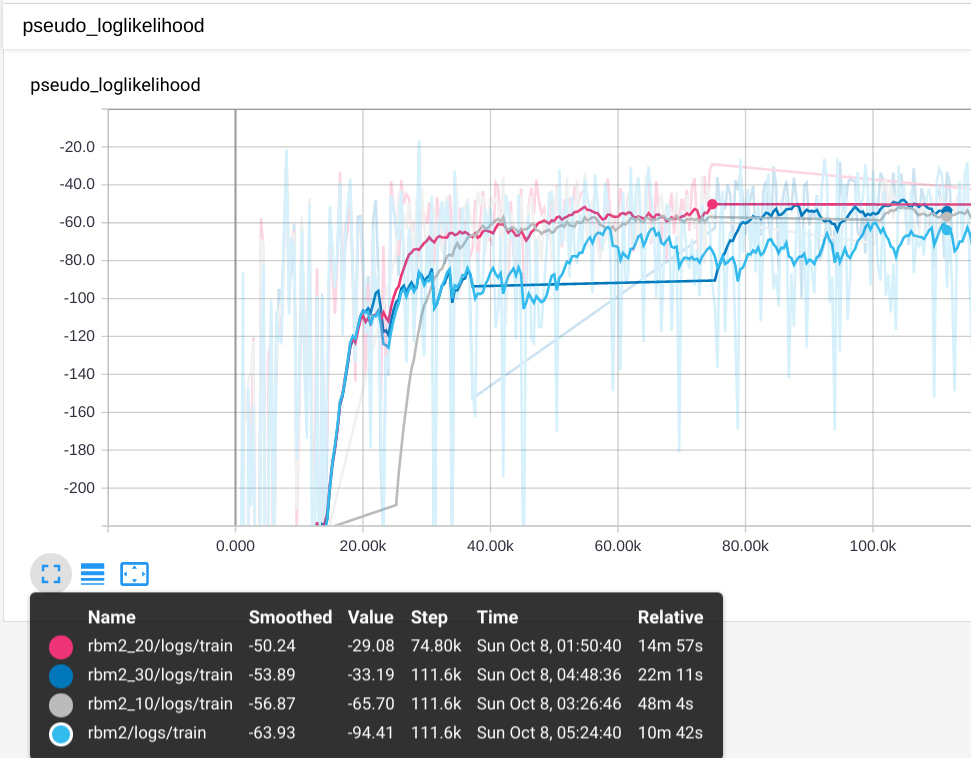
\includegraphics[width=4.2in]{dbm-mnist/rbm2_pll.png}
\\[1em]
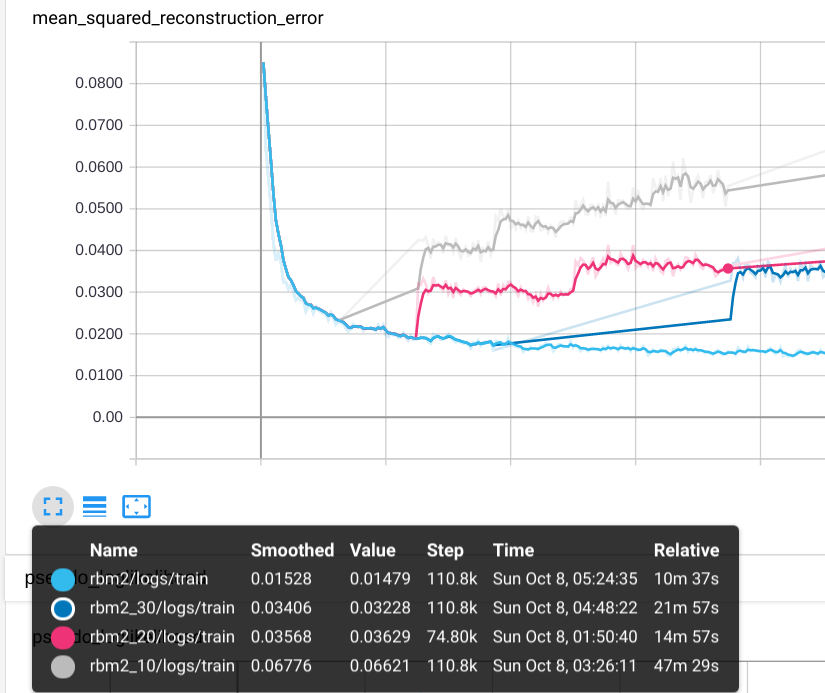
\includegraphics[width=4.2in]{dbm-mnist/rbm2_msre.png}
\caption{PLL and reconstruction error for RBM \#2 trained on extracted features $\mb{q}_i=p(\mb{h}|\mb{v}=\mb{x}_i; \bs{\psi})$ using RBM \#1 trained on MNIST. $\texttt{rbm\_n}$ means every $n$ epochs number of Gibbs sampling increased by 1, and learning rate $\alpha_t\leftarrow \frac{\alpha_0}{n}$. This approach \cite{dbm_code, salakhutdinov2007restricted} has quite noticeably higher PLL compared to CD-k with constant $k$ (both 1 or higher).}
\end{mdframed}
\end{figure}

\clearpage

\begin{figure}[h]
\begin{mdframed}
\centering
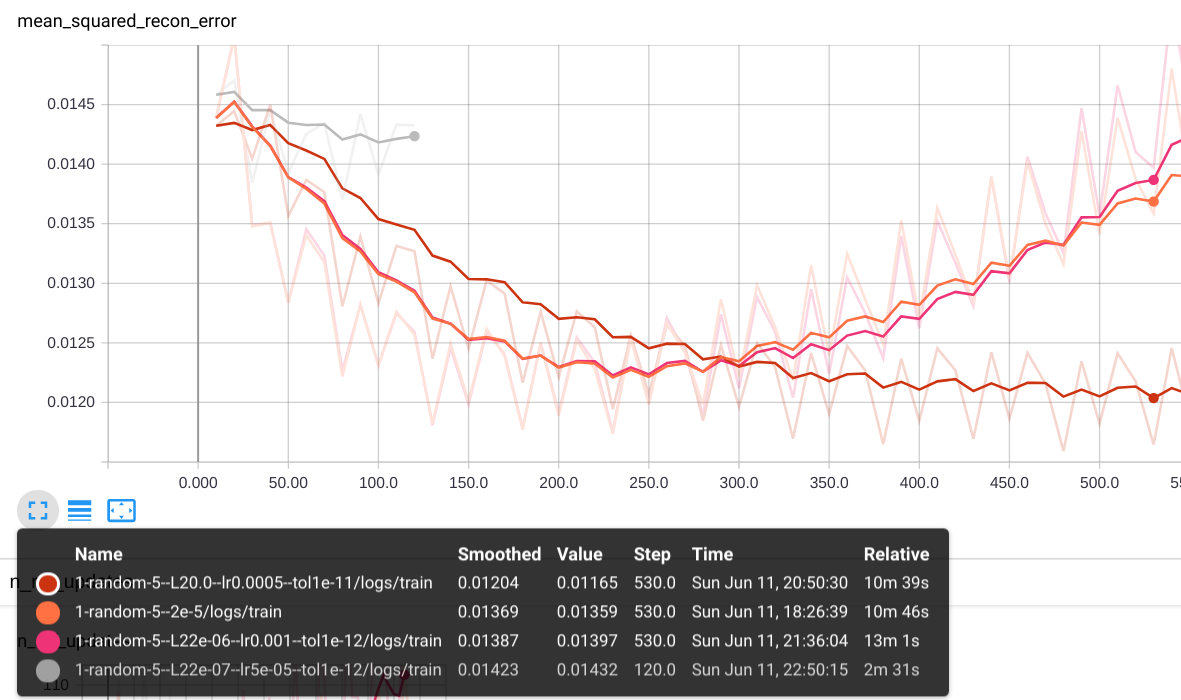
\includegraphics[width=6in]{dbm-mnist/L2_5k.png}
\caption{This illustrates how the use of L2 weight decay harms joint training of DBM in terms of MSRE (no matter how small $\lambda$ is). \u{The intuition} here is when weights are not trained well enough for them to be useful for modeling the data, the weight decay term will drive them to become very small, and they will never have an opportunity to recover. In \cite{goodfellow2013joint} and \cite{goodfellow2013multi} the authors had the same issue and suggested to use \emph{maxnorm} regularization instead. Trained on random subset of 5k images.}
\end{mdframed}
\end{figure}

\clearpage

\begin{figure}[h]
\begin{mdframed}
\centering
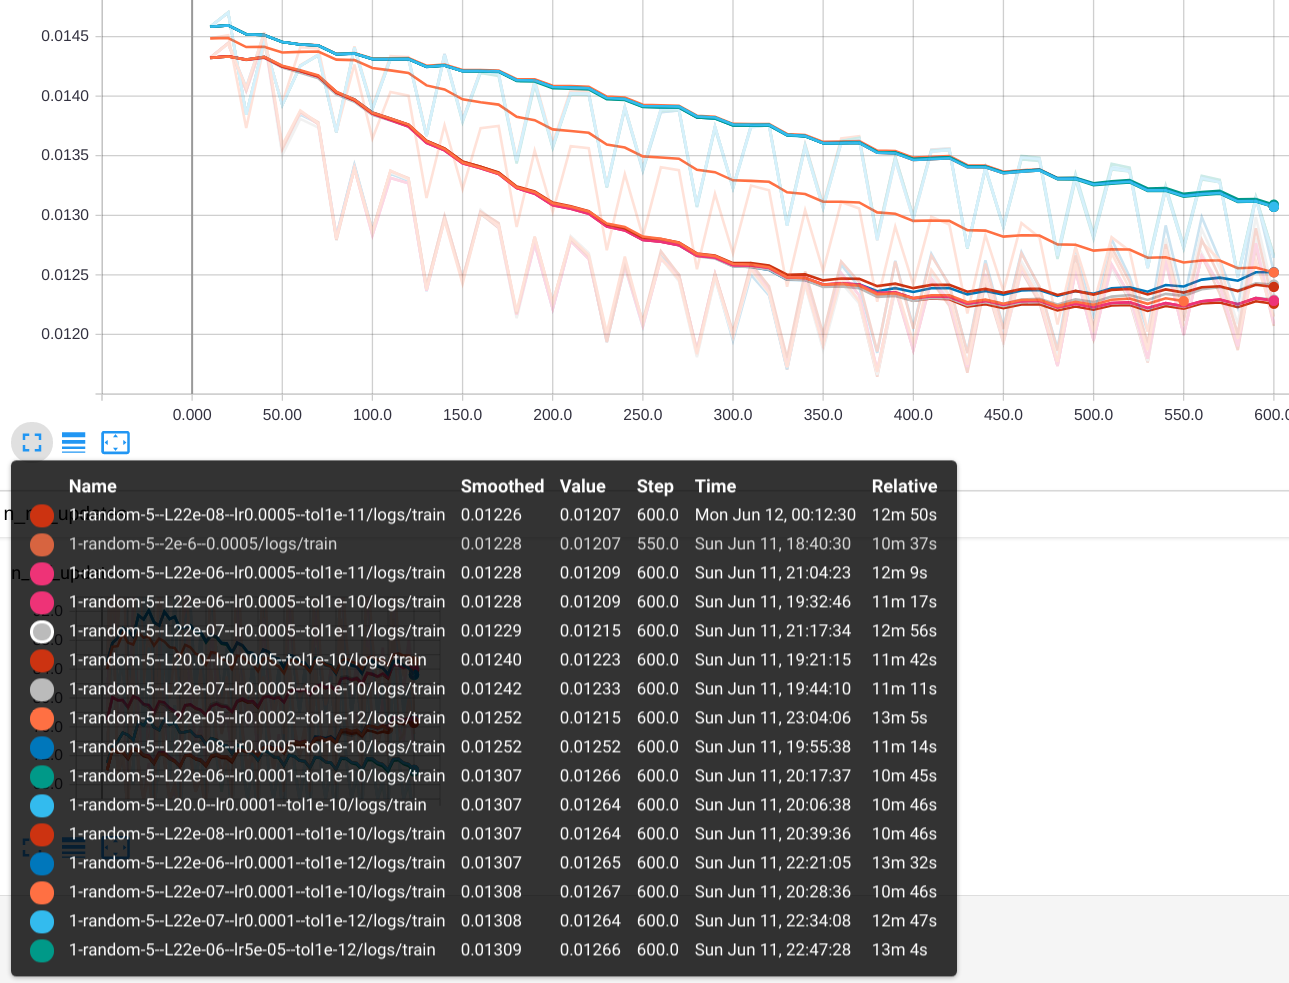
\includegraphics[width=4.6in]{dbm-mnist/L2_lr_tol_5k.png}
\\[2em]
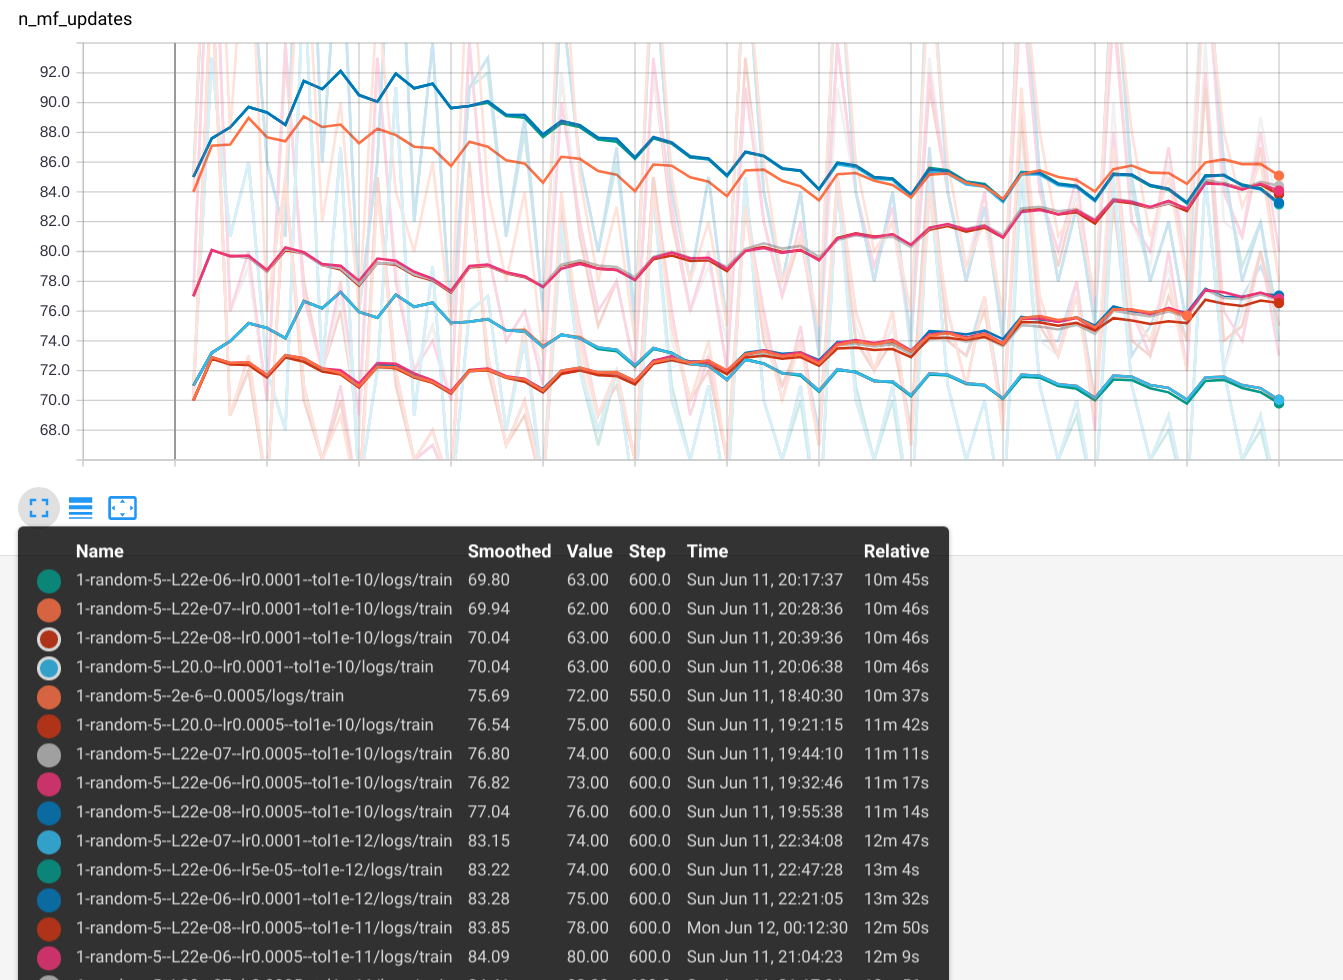
\includegraphics[width=4.6in]{dbm-mnist/n_mf_upd_5k.png}
\caption{The effect of various choices of L2 weight decay coefficient, learning rate and desired mean field tolerance in terms of reconstruction error and number of mean-filed updates to achieve desired tolerance on random subset of 5k images.}
\end{mdframed}
\end{figure}

\clearpage

\begin{figure}[h]
\begin{mdframed}
\centering
\includegraphics[width=4.6in]{dbm-mnist/lr_l2_maxnorm_10k.png}
\\[0.5em]
\includegraphics[width=4.6in]{dbm-mnist/l2_m_lr_n_bin_10k.png}
\caption{\emph{Top}: the effect of various choices of L2 weight decay coefficient, learning rate, maxnorm constraint and number of Gibbs steps on reconstruction error on random subset of 10k images from MNIST; 20 mean-filed updates, 100 particles, momentum $0.5\rightarrow 0.9$. \emph{Bottom}: the same, but on \u{binarized} version of MNIST, as suggested in \cite{goodfellow2012joint}.}
\end{mdframed}
\end{figure}

\clearpage

\begin{figure}[h]
\begin{mdframed}
\centering
\includegraphics[width=3in]{dbm-mnist/mf_approaches.png}
\quad
\includegraphics[width=2.5in]{dbm-mnist/parallel_gibbs.jpg}
\\[2em]
\includegraphics[width=4.5in]{dbm-mnist/n_mf_approaches.png}
\caption{\emph{Top left}: Various approaches on particles and variational parameters initialization to speedup mean-field convergence I've tried. Numbers of mean-filed updates are meant to achieve $10^{-11}$ tolerance. \tb{In sum}: it is always better to initialize \u{all} particles (including hidden ones) from the training data (hidden particles on the first level, for instance, should be initialized from the extracted fratures $\mb{q}_i=p(\mb{h}|\mb{v}=\mb{x}_i;\bs{\psi})$ from the first pre-trained RBM. Not resetting variation parameters between different gibbs updates is also slightly faster than bottom-up approximate inference described in \cite{salakhutdinov2009deep, salakhutdinov2010efficient}. It is thus a combination of these two best approaches (approx. inference + not resetting) is implemented in \texttt{DBM} class. Notwithstanding, the results (in terms of reconstruction error) were pretty robust to the exact number of mean-field updates: similar when used 10 or 25 mean-field updates. \emph{Top right}: I also tried "parallel" version of Gibbs sampling. One mean-field update was faster ($\approx 1.1-1.2$) but the total number of them was nearly twice as many. \emph{Bottom}: dynamics of mean field updates for various approaches. See also excel table. Experiments were tried on random subset 10k images.}
\end{mdframed}
\end{figure}

\clearpage

\begin{figure}[h]
\begin{mdframed}
\centering
\includegraphics[width=5.6in]{dbm-mnist/filters.png}
\\[2em]
\includegraphics[width=5.6in]{dbm-mnist/samples.png}
\caption{Best model trained on full MNIST in this phase in terms of the generated samples quality. 2nd layer filters are visualized using method of \emph{weighted linear combinations} \cite{erhan2009visualizing}. \tb{\emph{Hyperparams}}: 100 particles, 25 mean-filed updates, 1 Gibbs step per iter, mean-field tolerance $10^{-7}$, momentum $0.5\rightarrow 0.9$, learning rate $5\cdot10^{-4}\rightarrow 10^{-5}$ by dividing by $(1.000015)^{600}$ each epoch, 200 epochs, batch-size 100, L2 $=10^{-7}$, maxnorm $=4$; sample all visible and hidden states.
}
\end{mdframed}
\end{figure}

\clearpage

\begin{figure}[h]
\begin{mdframed}
\centering
\includegraphics[width=2in]{dbm-mnist/samples_0k.png}
\quad
\includegraphics[width=2in]{dbm-mnist/samples_25k.png}
\quad
\includegraphics[width=2in]{dbm-mnist/samples_50k.png}
\\[2em]
\includegraphics[width=2in]{dbm-mnist/samples_75k.png}
\quad
\includegraphics[width=2in]{dbm-mnist/samples_100k.png}
\quad
\includegraphics[width=2in]{dbm-mnist/samples_125k.png}
\\[2em]
\includegraphics[width=2in]{dbm-mnist/samples_150k.png}
\quad
\includegraphics[width=2in]{dbm-mnist/samples_175k.png}
\quad
\includegraphics[width=2in]{dbm-mnist/samples_200k.png}
\caption{This illustrates how correlated generated samples are between one another because the approach used to generate them is MCMC-based one}.
\end{mdframed}
\end{figure}

\clearpage
\subsubsection{After sparsity targets, AIS are implemented}
After AIS is implemented, now it is possible to quantitatively evaluate DBM performance. To do this, I cross-validated 216 models with various hyperparameters on small held-out validation set $\rightarrow$ chose best values of hyperparameters based on ELBO estimation and quality of samples $\rightarrow$ repeated for 54 models with larger validation set $\rightarrow$ 4 $\rightarrow$ 1.
\\
\tb{Interesting observation}: AIS is (much) more accurate for better models and which are trained longer.
Results:

\begin{figure}[h]
\begin{mdframed}
\centering
\includegraphics[width=2.5in]{dbm-mnist-latest/rbm1.png}
\quad
\includegraphics[width=2.5in]{dbm-mnist-latest/rbm2.png}
\\[2em]
\includegraphics[width=2.5in]{dbm-mnist-latest/W1_joint.png}
\quad
\includegraphics[width=2.5in]{dbm-mnist-latest/W2_joint.png}
\caption{Weight filters}.
\end{mdframed}
\end{figure}

\clearpage
\begin{figure}[h]
\begin{mdframed}
\centering
\includegraphics[width=2.8in]{dbm-mnist-latest/mnist.png}
\quad
\includegraphics[width=2.8in]{dbm-mnist-latest/samples.png}
\\[2em]
\includegraphics[width=5.6in]{dbm-mnist-latest/msre.png}
\caption{\emph{Top}: random subset of training data and generated samples by DBM. \emph{Bottom}: MSRE of DBM}.
\end{mdframed}
\end{figure}

\clearpage
\newpage
\subsection{Experiments on CIFAR-10}
\subsubsection{Before sparsity targets, AIS; naive training of Gaussian RBM}
\u{Architecture}: 3072-5000-1000 Gaussian-Bernoulli-Multinomial DBM.
\\[0.5em]
\u{Preprocessing}: Zeroing 1000 least significant variance directions as in \cite{krizhevsky2009learning}.
\clearpage

\begin{figure}[h]
\begin{mdframed}
\centering
\includegraphics[width=5in]{dbm-cifar/instab.png}
\\[2em]
\includegraphics[height=2in]{dbm-cifar/mu_before.png}
\quad
\includegraphics[height=2in]{dbm-cifar/mu_1_before.png}
\caption{After pre-training during the joint training severe instabilities occured unless an extremely small learning rate was used. After inspection of distribution of variational parameters (in first and second hidden layers), \u{the reason became clear}: the total input to first layer hidden units was too large $\Rightarrow$ "overshoot" of sigmoid units. For training 5k random images were used.}
\end{mdframed}
\end{figure}

\clearpage

\begin{figure}[h]
\begin{mdframed}
\centering
\includegraphics[width=5in]{dbm-cifar/instab_resolved.png}
\\[2em]
\includegraphics[height=2in]{dbm-cifar/mu_after.png}
\quad
\includegraphics[height=2in]{dbm-cifar/mu_1_after.png}
\caption{\emph{Top}: reconstruction error when the total input from Multinomial layer were multiplied by $\frac{1}{\sqrt{M}}$ and $\frac{\log(1+M)}{M}$ from previous experiment. \emph{Bottom}: distribution of variational parameters in first and second hidden layers after $\frac{1}{\sqrt{M}}$ scaling were applied.}
\end{mdframed}
\end{figure}

\clearpage

\begin{figure}[h]
\begin{mdframed}
\centering
\includegraphics[width=6in]{dbm-cifar/mrbm.png}
\caption{Reconstruction error of Multinomial RBM trained on extracted features $\mb{q}_i=p(\mb{h}|\mb{v}=\mb{x}_i; \bs{\psi})$ of Gaussian RBM on full dataset.}
\end{mdframed}
\end{figure}

\clearpage

\begin{figure}[h]
\begin{mdframed}
\centering
\includegraphics[width=5.2in]{dbm-cifar/filters.png}
\\[2em]
\includegraphics[width=5.2in]{dbm-cifar/samples.png}
\caption{Best model trained on full CIFAR-10 dataset in this phase. 2nd layer filters are visualized using method of \emph{weighted linear combinations} \cite{erhan2009visualizing}. \tb{\emph{G-RBM Hyperparams}}: L2 0.001, batch size 100, 99 epochs, lr 0.0005, momentum $0.5\rightarrow 0.9$, 1 Gibbs step, w\_std 0.0008, biases to 0, $\bs{\sigma}$ from data; sample both visible and hidden states. \tb{\emph{M-RBM Hyperparams}}: L2 0.05, batch size 100, 118 epochs, learning rate 0.0001, momentum $0.5\rightarrow 0.9$, 1 Gibbs step, number of samples $M=K=1000$, w\_std 0.01, biases to zero; sample only hidden states (for visible use probabilities w/o sampling); no scaling of total input. \tb{\emph{DBM Hyperparams}}: 100 particles, initialize from data for all layers, 1 Gibbs step, 25 mean-field updates ($10^{-13}$ tolerance), momentum $0.5\rightarrow 0.9$, learning rate $9\cdot10^{-5}\rightarrow 10^{-5}$ by dividing by $(1.000015)^{600}$ each epoch, 200 epochs, batch size 50, L2 $=0$, max norm $=2$; sample all visible and hidden states.}
\end{mdframed}
\end{figure}

\clearpage
\newpage
\subsubsection{"naive" training of Gaussian RBM}
\begin{figure}[h]
\begin{mdframed}
\centering
\includegraphics[width=2.5in]{dbm-cifar-naive/grbm.png}
\quad
\includegraphics[width=2.5in]{dbm-cifar-naive/mrbm.png}
\\[2em]
\includegraphics[width=2.5in]{dbm-cifar-naive/W1_joint.png}
\quad
\includegraphics[width=2.5in]{dbm-cifar-naive/W2_joint.png}
\caption{Weight filters}.
\end{mdframed}
\end{figure}

\clearpage
\subsubsection{"naive" training of Gaussian RBM}
\begin{figure}[h]
\begin{mdframed}
\centering
\includegraphics[width=3.5in]{dbm-cifar-naive/grbm_msre.png}
\quad
\includegraphics[width=2.4in]{dbm-cifar-naive/grbm_feg.png}
\\[4em]
\includegraphics[width=5.4in]{dbm-cifar-naive/dbm_msre.png}
\caption{\emph{Top}: reconstruction error and free nergy gap of Gaussian RBM. \emph{Bottom}: reconstruction error of DBM after joint training.}.
\end{mdframed}
\end{figure}

\clearpage
\newpage
\subsubsection{advanced training of Gaussian RBM}
In this experiment DBM was pretrained and trained on augmented (10 times) CIFAR-10 dataset with shifts by 1 pixel in all directions and mirroring. Also, Gaussian RBM was initialized from 26 small RBMs trained on patches of images, as in \cite{krizhevsky2009learning}, see Fig. \ref{fig:small_rbms}.
\\
\tb{Observation}: in \cite{krizhevsky2009learning} when they initialize large weight matrix, they leave zeros in places where there were no connections in small RBMs during pre-training. I found that using instead random values with small standard deviation (around $10^{-5}$) yield slightly better performance with filters of large RBM smoothed in the neighborhood of corresponding filter from small RBM.
\begin{figure}[h]
\begin{mdframed}
\includegraphics[scale=0.75]{img/small_rbms.png}
\centering
\caption{Pre-training 26 RBMs on patches of images. 26-th RBM was trained on subsampled versions of images.}
\label{fig:small_rbms}
\end{mdframed}
\end{figure}

\clearpage
\begin{figure}[h]
\begin{mdframed}
\centering
\includegraphics[width=1.6in]{dbm-cifar-latest/rbm_small_0.png}
\quad
\includegraphics[width=1.6in]{dbm-cifar-latest/rbm_small_2.png}
\\[1em]
\includegraphics[width=1.6in]{dbm-cifar-latest/rbm_small_10.png}
\quad
\includegraphics[width=1.6in]{dbm-cifar-latest/rbm_small_20.png}
\\[1em]
\includegraphics[width=6.4in]{dbm-cifar-latest/small_rbms.png}
\caption{\emph{Top}: Weight filters. \emph{Bottom}: reconstruction error and free energy gap of small RBMs. Notice different groups of RBMs based on their reconstruction errors. The lowest ($\approx$0.03) one has RBM which was trained on subsampled images. Next two ($\approx$0.078) were trained on top left and right corners of the images, which are the smoothest among all patches. Next 4 ($\approx$0.092) RBMs were trained on patches which are direct neighbors to top left and right, and after that come all the others.}.
\end{mdframed}
\end{figure}

\clearpage
\begin{figure}[h]
\begin{mdframed}
\centering
\includegraphics[width=2.2in]{dbm-cifar-latest/grbm.png}
\quad
\includegraphics[width=2.2in]{dbm-cifar-latest/mrbm.png}
\\[2em]
\includegraphics[width=2.2in]{dbm-cifar-latest/W1_joint.png}
\quad
\includegraphics[width=2.2in]{dbm-cifar-latest/W2_joint.png}
\\[2em]
\includegraphics[width=2.2in]{dbm-cifar-latest/cifar10.png}
\quad
\includegraphics[width=2.2in]{dbm-cifar-latest/samples.png}
\caption{\emph{Top}: Weight filters. \emph{Bottom}: random subset of training data and generated samples by DBM.}.
\end{mdframed}
\end{figure}

\clearpage
\begin{figure}[h]
\begin{mdframed}
\centering
\includegraphics[width=6.4in]{dbm-cifar-latest/grbm_metrics.png}
\\[6em]
\includegraphics[width=6in]{dbm-cifar-latest/dbm_msre.png}
\caption{\emph{Top}: reconstruction error and free energy gap of Gaussian RBM \emph{Bottom}: reconstruction error of DBM.}.
\end{mdframed}
\end{figure}

	\newpage
\section{Some conclusions}
\begin{itemize}
	\gooditem RBM, DBM: small models (1-2 layers) yet powerful;
	\gooditem large enough to overfit (millions of learnable parameters) but they don't, thank to in-built regularizer / information bottleneck -- random sampling;
	\gooditem RBM, DBM and other energy-based models are quite principled from theoretical perspective: structure, distribution of visible and hidden units and basically everything is determined by and can be derived from energy function;
	\gooditem for inference no need to input any additional information, as opposed to e.g. VAE (where for inference we need input latent code $\mb{z}$, and if we are not careful enough we may infer $\mb{x}$ somewhere between the modes which will result in unlikely image if the model was trained on images, unless something like cVAE has been used); this is not happen with RBM/DBM, we simply run Gibbs sampler using trained weights, and on decently trained model, most of the time particles output valid e.g. digits (MNIST);
	\baditem samples are highly correlated between one another, therefore many Gibbs steps need to be performed to obtain image from different mode ("slow-mixing problem");
	\baditem hard to tune, many hyperparameters, and they are not transferable between models, units' distriutions or tasks
	\baditem \u{really} hard to tune for complex tasks, many tricks;
	\baditem in papers lots of details omitted: exact hyperparameters in most cases, biases are omitted for "simplicity" in most papers etc.;
	\baditem hardly any working and complete examples of DBM codes;
	\item most of the features can be extracted in unsupervised manner, and then only limited amount of labeled information can be used to slightly adjust the layers of features already discovered by the DBM;
	\item RBMs and DBMs, especially classes for stochastic units could have been implemented purely in \texttt{edward}.
\end{itemize}


	\newpage
	\pdfbookmark{References}{references}
	
	\nocite{*}
	\bibliographystyle{ieee}
	\bibliography{bib}

\end{document}